% !TeX spellcheck = en_GB

%%%%%%%%%%%%%%%%%%%%%%%%%%%%%%%%%%%%%%%%%%%%%%%%%%%%%%%%%%%%%%%%%%%%%%%%
\chapter{Plug-in}
\label{chap:Plugin}

This chapter describes the goals of the plug-in and how the implementation accommodates these goals. It also includes the thought process behind some architectural decisions that were made.

At the end, alternative solutions that were taken into consideration but eventually abandoned are described. They complement the reasoning about the final architecture.

%%%%%%%%%%%%%%%%%%%%%%%%%%%%%%%%%%%%%%%%%%%%%%%%%%%%%%%%%%%%%%%%%%%%%%%%
\section{Goals}
\label{sec:goals}

This section lists which goals the plug-in should meet. Each goal will be marked with a number which will later be reused in Section \ref{sec:conclusion} to summarize how the goals were met.

\begin{enumerate}[label=(\labelenum{G}{{\arabic*}})]
  \item \textbf{Easy-to-understand visualization of the encryption process}\\
The main goal of the plug-in was to teach students how the ChaCha cipher family encrypts messages. Therefore, the visualization should be easy to follow without much prior knowledge about ciphers.
  \item \textbf{Visualization of the diffusion property}\\
To get a better understanding how the cipher hides the relationship between the ciphertext and the plaintext, the plug-in should contain a visualization of the diffusion property. To achieve this, the user should be able to flip bits of the input values.
  \item \textbf{Support for all variants of the cipher family}\\
The plug-in should support 128-bit and 256-bit keys and the default 64-bit counter and 64-bit initialization vector. Since the Internet Engineering Task Force (IETF) introduced a slightly modified version of the cipher which has a 32-bit counter and a 96-bit initialization vector, the plug-in should also support these values. Finally, the user should also be able to choose between 8, 12 or 20 rounds.
\end{enumerate}

%%%%%%%%%%%%%%%%%%%%%%%%%%%%%%%%%%%%%%%%%%%%%%%%%%%%%%%%%%%%%%%%%%%%%%%%
\section{Implementation Details}
\label{sec:implementationDetails}

This section details how the goals described in the previous section were achieved. \\
In the first subsection, the key features of the plug-in are described to give a rough overview what a user can expect from the actual plug-in implementation. \\
The second subsection will then explain the user interface which is used to navigate through the plug-in and communicate to the user what is currently happening inside the cipher. \\
The last subsection then goes into technical details to explain how the plug-in internally was designed to make the user interface behave as it does.

%%%%%%%%%%%%%%%%%%%%%%%%%%%%%%%%%%%%%%%%%%%%%%%%%%%%%%%%%%%%%%%%%%%%%%%%

\subsection{Key Features}
\label{sec:keyFeatures}

\begin{figure}
\centering
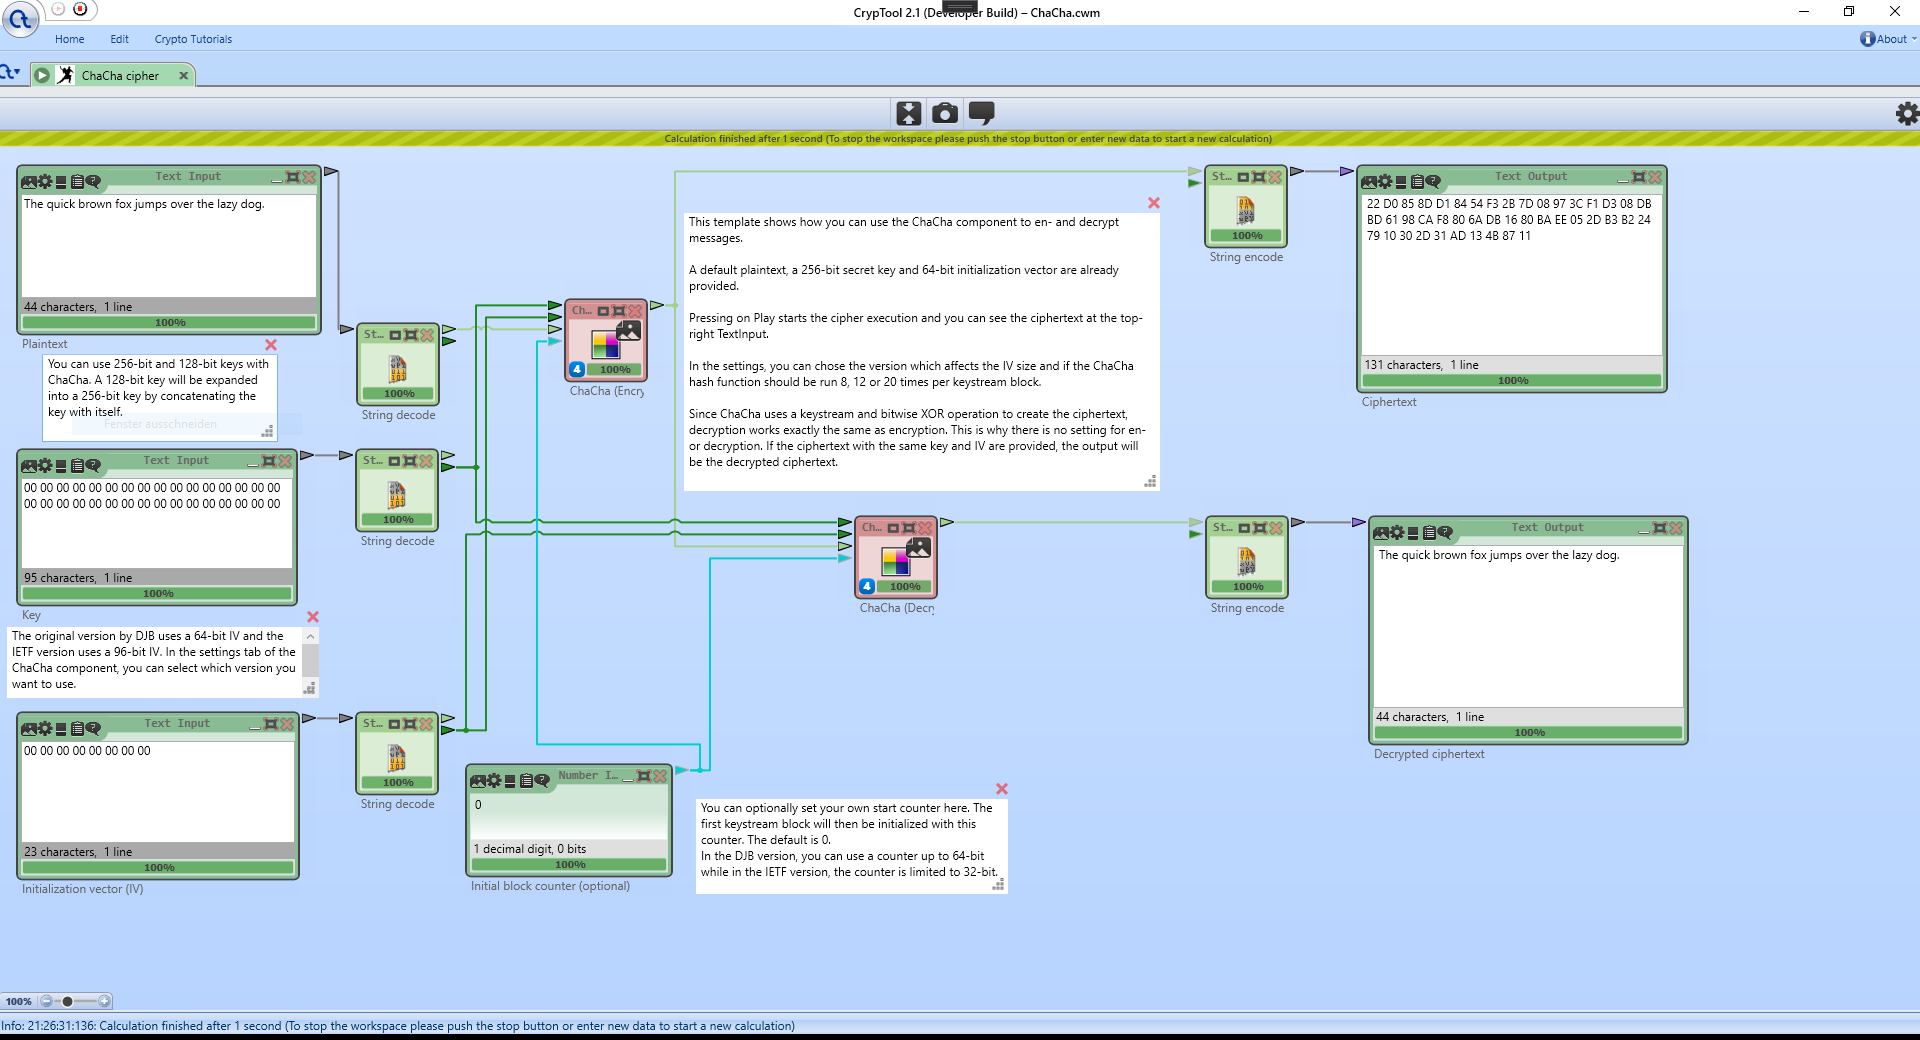
\includegraphics[width=\textwidth]{figures/ct2/plugin-template.png}
\caption[ChaCha CT2 template]{CT2 template for the ChaCha plug-in}
\label{fig:plugin.template}
\end{figure}

The plug-in offers the user the ability to input his own plaintext, key, initialization vector and initial counter using the concept of visual programming (around which CT2 is built) as one can see in Figure \ref{fig:plugin.template}. The counter is optional and defaults to zero. These values are then used to visualize the cipher execution comprehensively. Descriptions complement the visualization by providing information about what is happening. \\
As mentioned in Section \ref{sec:goals}, if the user wants to see the diffusion property of the cipher, he can alter the key, initialization vector and counter on a dedicated page inside the plug-in. \\
The version (original DJB version or IETF version) and how often the ChaCha hash function should be run per keystream block can be chosen in the plug-in settings.

\subsection{User Interface}
\label{sec:userInterface}

This subsection will describe the layout and functionality of the user interface and the reasoning behind it. First, the parts of the user interface which all pages have in common will be explained. Afterwards, we will expand upon the interface differences between the individual pages.

\subsubsection{General interface structure}

All pages have a common interface layout which consists of three sections. Each section is inside an own dedicated row.

The first section implements the navigation to move between pages. It also shows the title of the current page.

The second section shows the content of the current page. The content is not always static since it can change by using the action navigation bar in the bottom section. This navigation bar includes buttons to go to the previous or next action, a slider for quicker action navigation, a text input to go to a given action and a indicator on which action the user currently is and how many actions there are in total on the current page. In Figure \ref{fig:statematrixpage}, you can see this navigation bar for the first time.

A slider was chosen over alternative solutions like individual buttons because a slider enables the user to quickly navigate through a page. This advantage  is best noticeable on the page about the ChaCha hash function where there are more than 3000 actions per keystream block. Fitting more than 3000 buttons on a single page was not feasible but would need pagination features such as showing the next set amount of buttons which would make quick navigation impossible. \\
The user can also enter a  number into the text input to the right of the slider to go to an action. But this text input is only more helpful than the slider if the user already knows the number of the action he wants to go to. If he does not, the slider creates a much better user experience. \\
If a page does not have actions, the action navigation is hidden but the space is still reserved for it to have a consistent canvas size for all pages.

What follows are sections which go into greater detail about each page which does not have fully static content. These pages are the Diffusion page, the State Matrix Initialization page and the ChaCha Hash Function page.

\begin{figure}
\centering
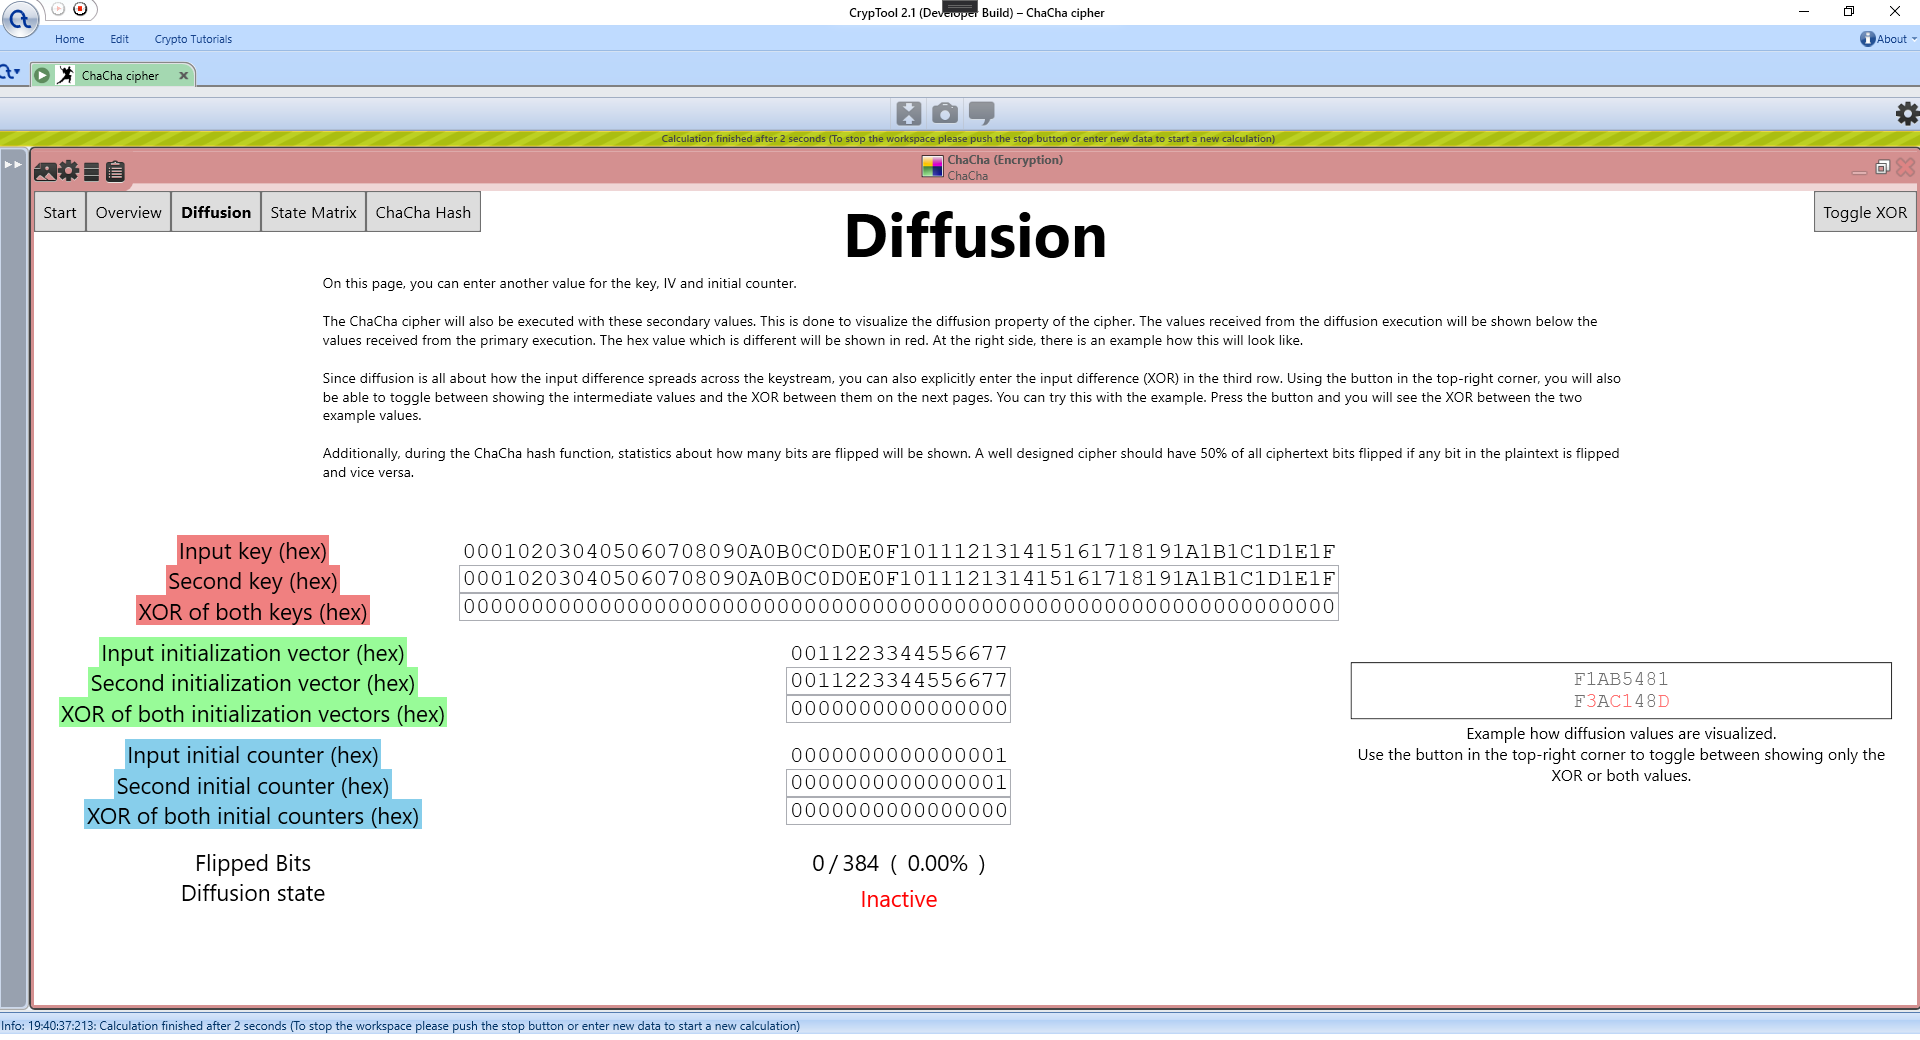
\includegraphics[width=\textwidth]{figures/ct2/all-pages/3-diffusion.png}
\caption{Diffusion page in its initial state}
\label{fig:diffusionpage}
\end{figure}

\subsubsection{Diffusion page}

The Diffusion page (Figure \ref{fig:diffusionpage}) is the dedicated page, as mentioned in Section \ref{sec:keyFeatures}, where the user can alter the key, initialization vector (IV) and initial counter in hexadecimal. They will be used to visualize the diffusion property. This means that during cipher execution, hexadecimal letters which are different are marked red. An example of this is shown on the Diffusion page at the right side.

Hexadecimal text inputs were chosen because alternatives like individual checkboxes for each bit (like in the DES visualization) or binary text inputs would have taken up a lot of canvas size because the key, counter and IV could be together 384-bit (if using a 256-bit key). This lost canvas size would have taken away the canvas size for other features like the example or would have made the page very crowded.

Unfortunately, using hexadecimal input fields made it harder to flip specific bits. This feature was necessary since when studying the diffusion property of a cipher, one is more interested in the difference of two values (XOR) during two cipher runs instead of the concrete values. The solution for this was to introduce a third input field where the user can explicitly input the XOR between the input value and the altered value. Additionally, if diffusion is active, the user can toggle if he wants to see the XOR and both concrete values during the cipher execution by using the button in the top-right corner of each page.

To help with the input, the input fields show an error message if the user entered invalid characters or a too large string since the hex strings for each value must be of equal size as the input value. If the hex string is too short, it gets left-padded with zeroes to align it with the primary value.

Last but not least, the amount of flipped bits is shown in the second to last row together with a state indication in the last row if the diffusion is active or not. The diffusion is active if at least one bit was flipped. This is shown in Figure \ref{fig:diffusion.active}.

\begin{figure}
\centering
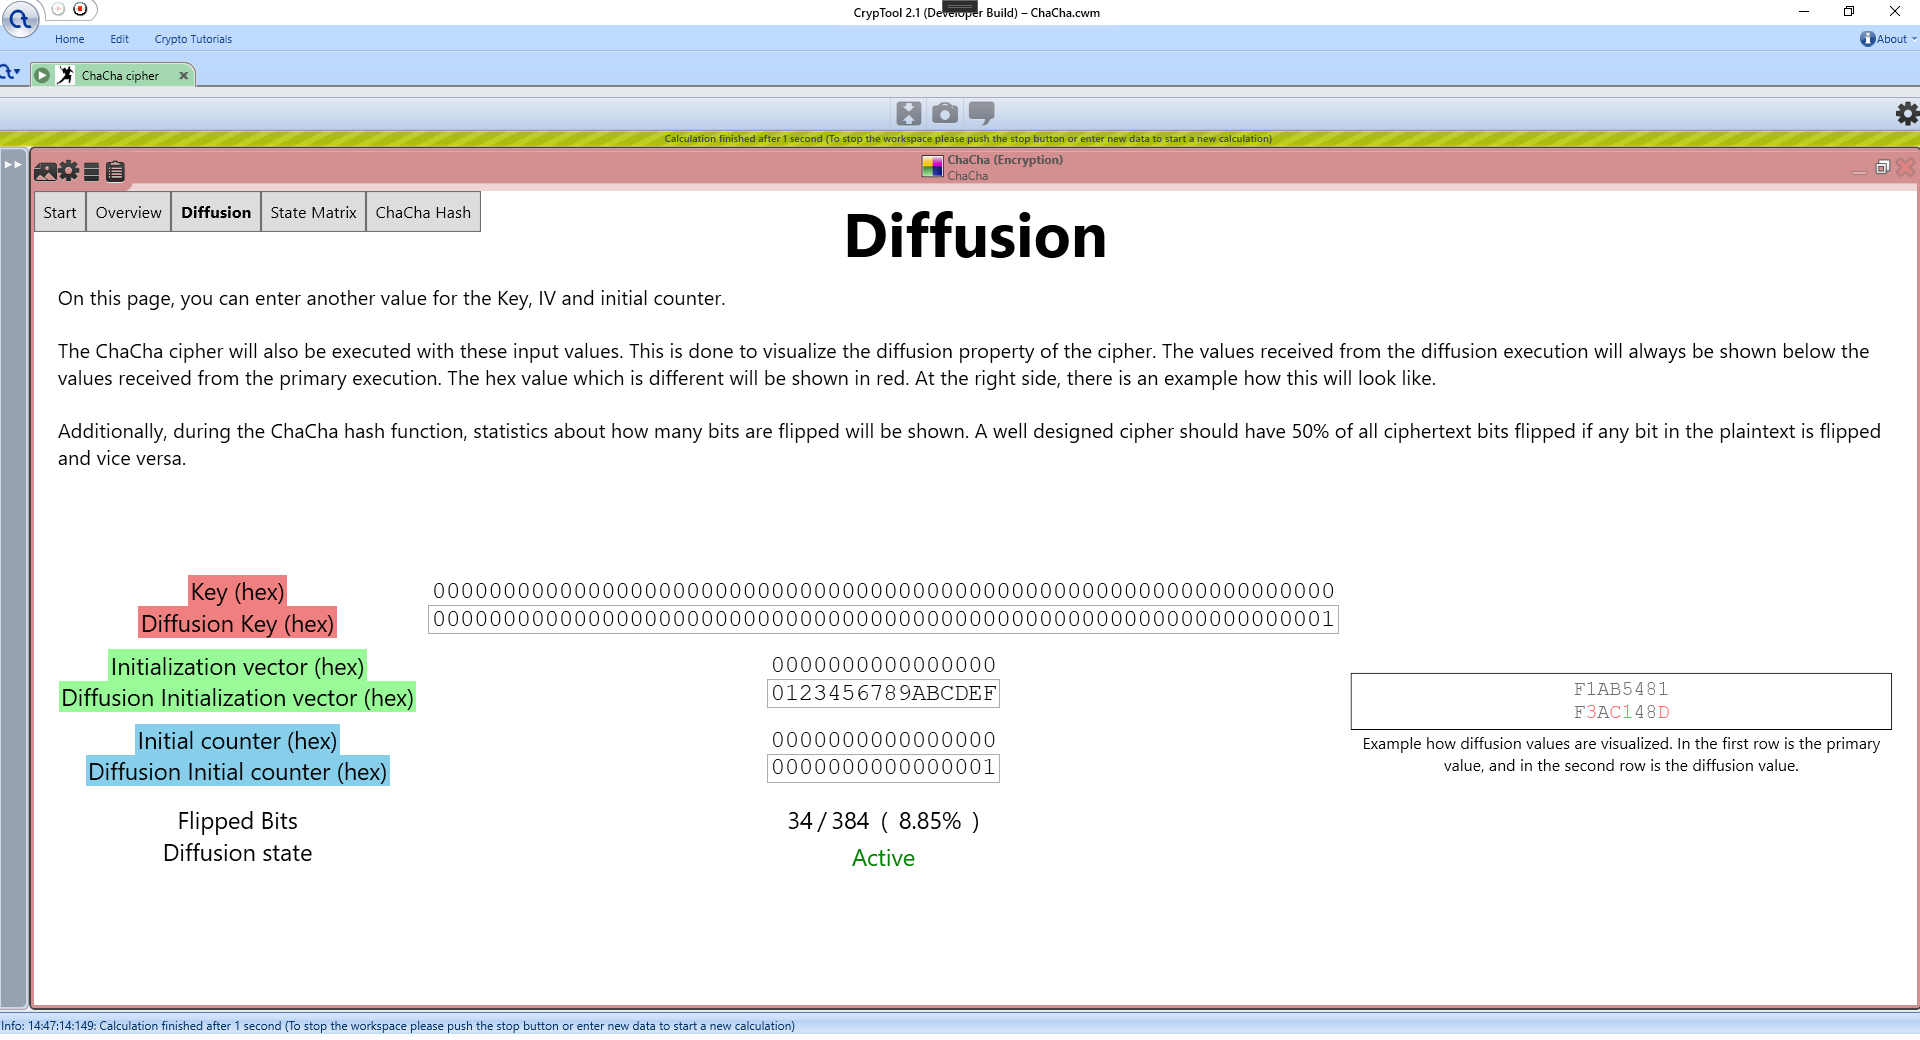
\includegraphics[width=\textwidth]{figures/ct2/diffusion/diffusion-active.png}
\caption{Diffusion page in its active state}
\label{fig:diffusion.active}
\end{figure}

\subsubsection{State Matrix Initialization page}

The State Matrix Initialization page shows the setup of the initial 512-bit state for the first keystream block. \\
In Figure \ref{fig:statematrixpage}, you can see the page in its initial state. In the top-left, you see the state. It is empty at the beginning because the initialization has not started yet. On the top-right, you see descriptions which inform the user about what the next steps are. At the bottom-left, the encoding will be visualized. At the bottom-right, the state parameters with their original values before encoding are shown. At the bottom above the slider are individual buttons to go to the start and end of each state parameter encoding.

\begin{figure}
\centering
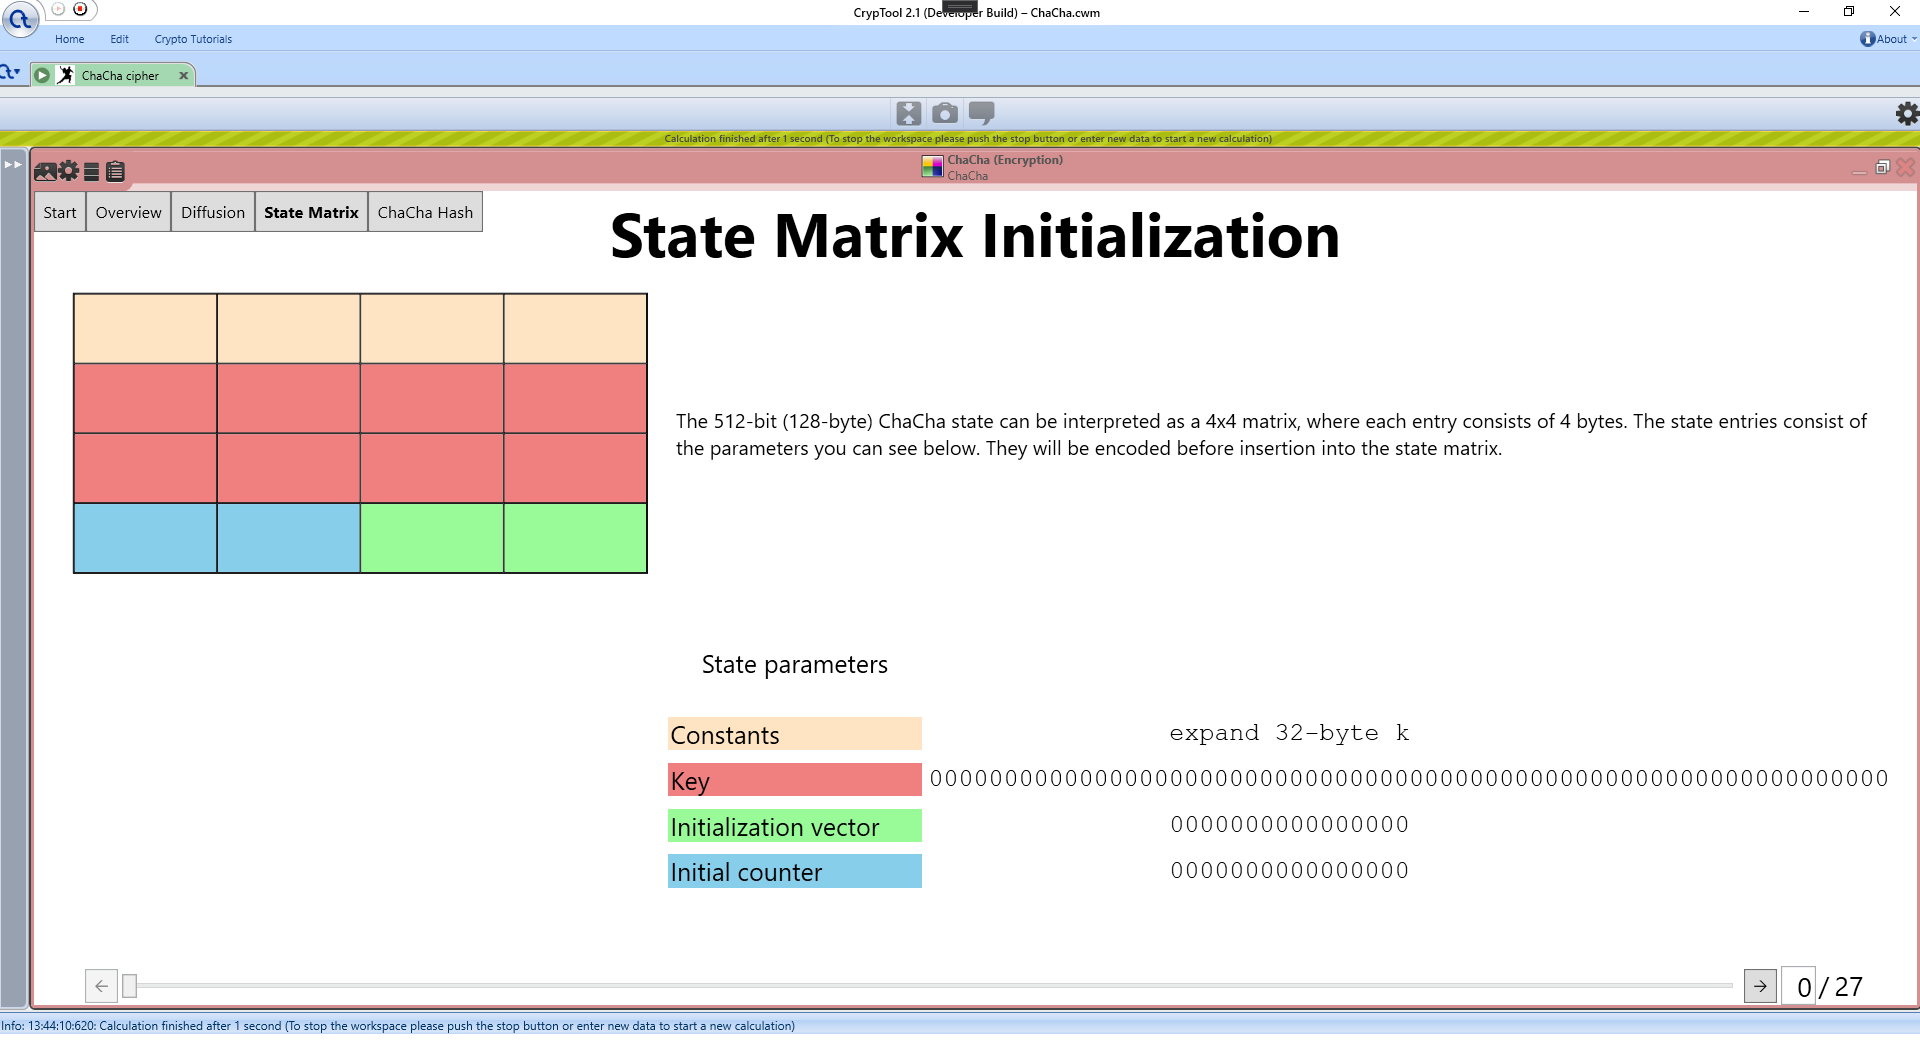
\includegraphics[width=\textwidth]{figures/ct2/all-pages/4-statematrix.png}
\caption{State Matrix Initialization page in its initial state}
\label{fig:statematrixpage}
\end{figure}

Only the construction of the state for the very first keystream block is shown on this page. This was done like this because interrupting the page flow by jumping back to the visualization of the state matrix initialization after each keystream block was not reasonable. Further, only the counter would be different for each state so setting up the state again would introduce a lot of noise to the visualization. The information which is provided to the user in the first and only state matrix initialization should be enough for him to construct all following initial states without further guidance. To achieve this, the focus for this page was on developing a comprehensive visualization of the encoding for each state parameter (constants, key, IV, counter).

In Figure \ref{fig:statematrix.encoding}, you can see the page state during the end of each state parameter encoding. For each encoding step which corresponds to a row in the encoding section, a page action has been implemented. This means that the user can follow along each encoding step-by-step in his own speed and is not overwhelmed by a lot of information.

First, the constants are encoded. Since they are shown in ASCII format in the state parameters section, they are first decoded to show the actual byte values. Then the 
bytes are split into 4 byte chunks whose order is then reversed in the last step. \\
Afterwards, the key is encoded. It is just split into 4 byte chunks whose order is then reversed. \\
When encoding the counter, the complete byte order is first reversed, and then it is split into 4 byte chunks whose byte order is then again reversed. \\
The last parameter is the IV. It is encoded exactly the same as the key. \\

\begin{figure}
\begin{subfigure}{\textwidth}
  \centering
  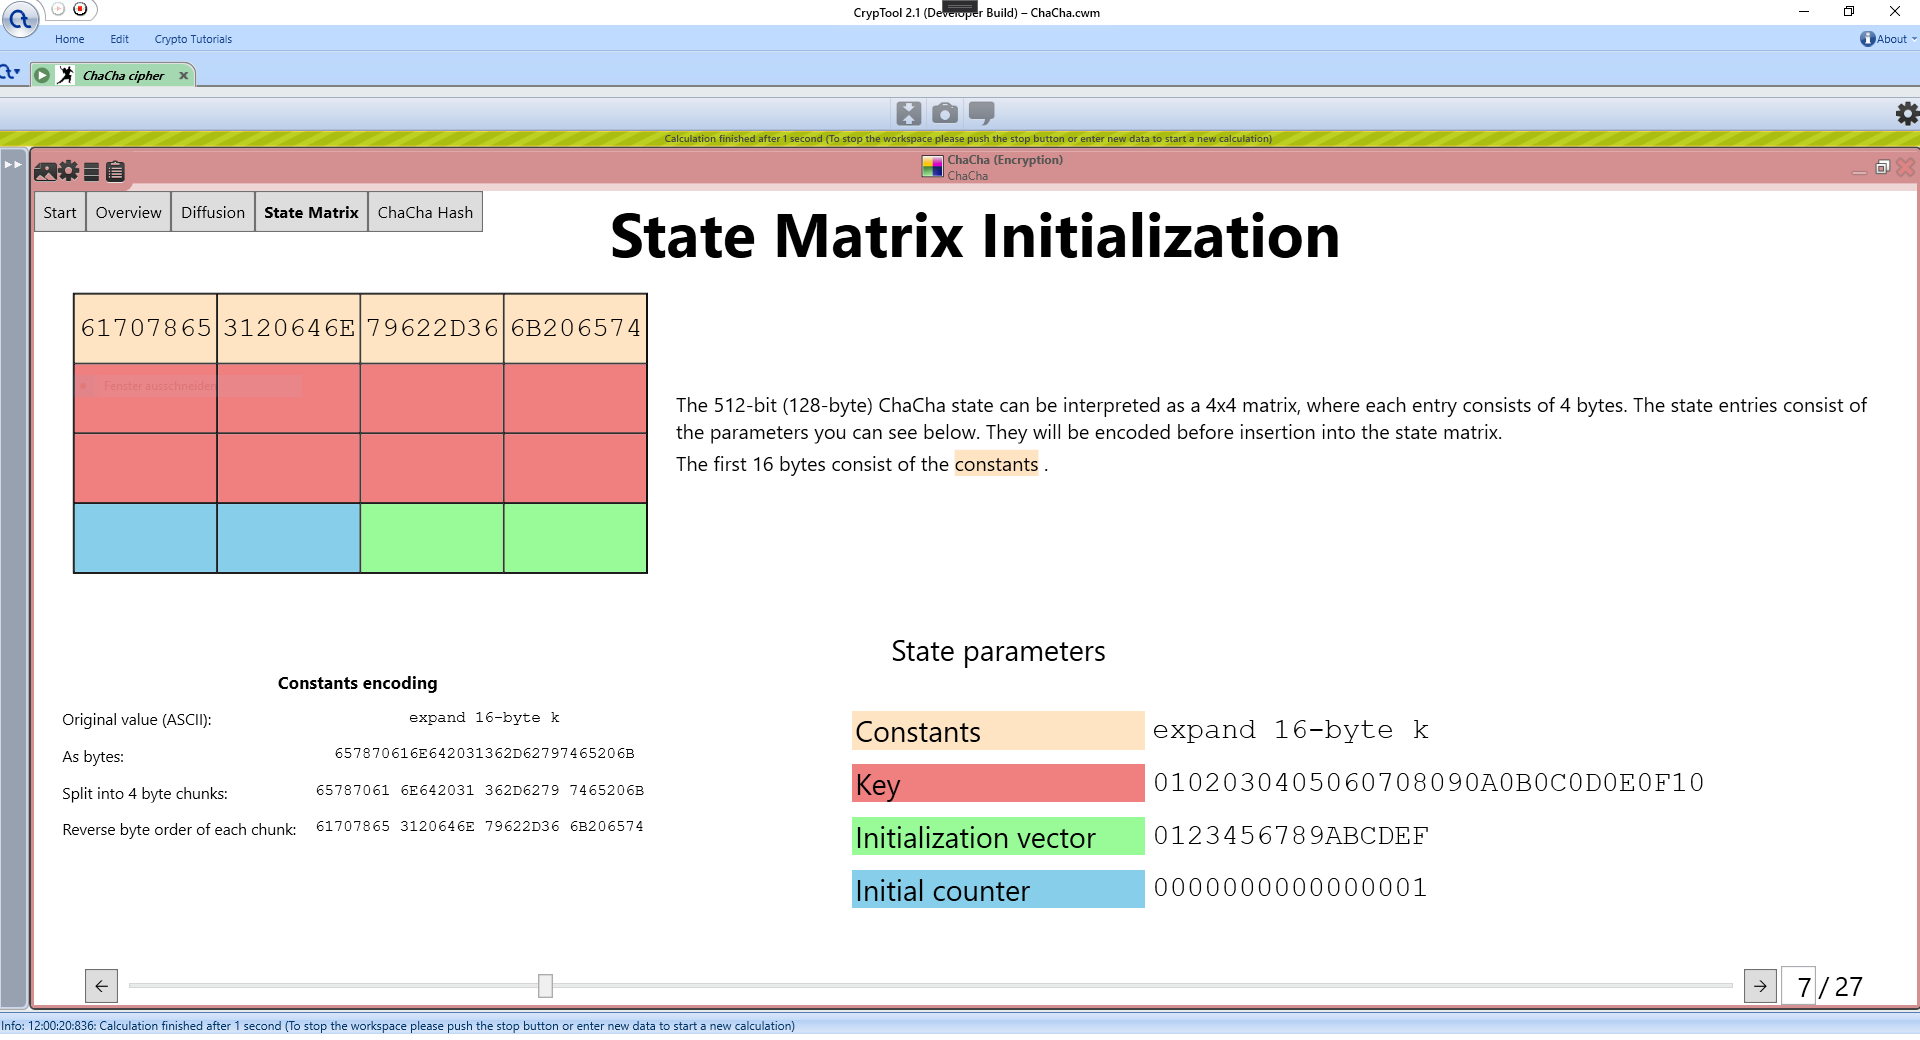
\includegraphics[width=\textwidth]{figures/ct2/state-matrix/1-state-matrix-constants.png}
  \caption{Constants encoding}
  \label{fig:statematrix.encoding.constants}
\end{subfigure}
\begin{subfigure}{\textwidth}
  \centering
  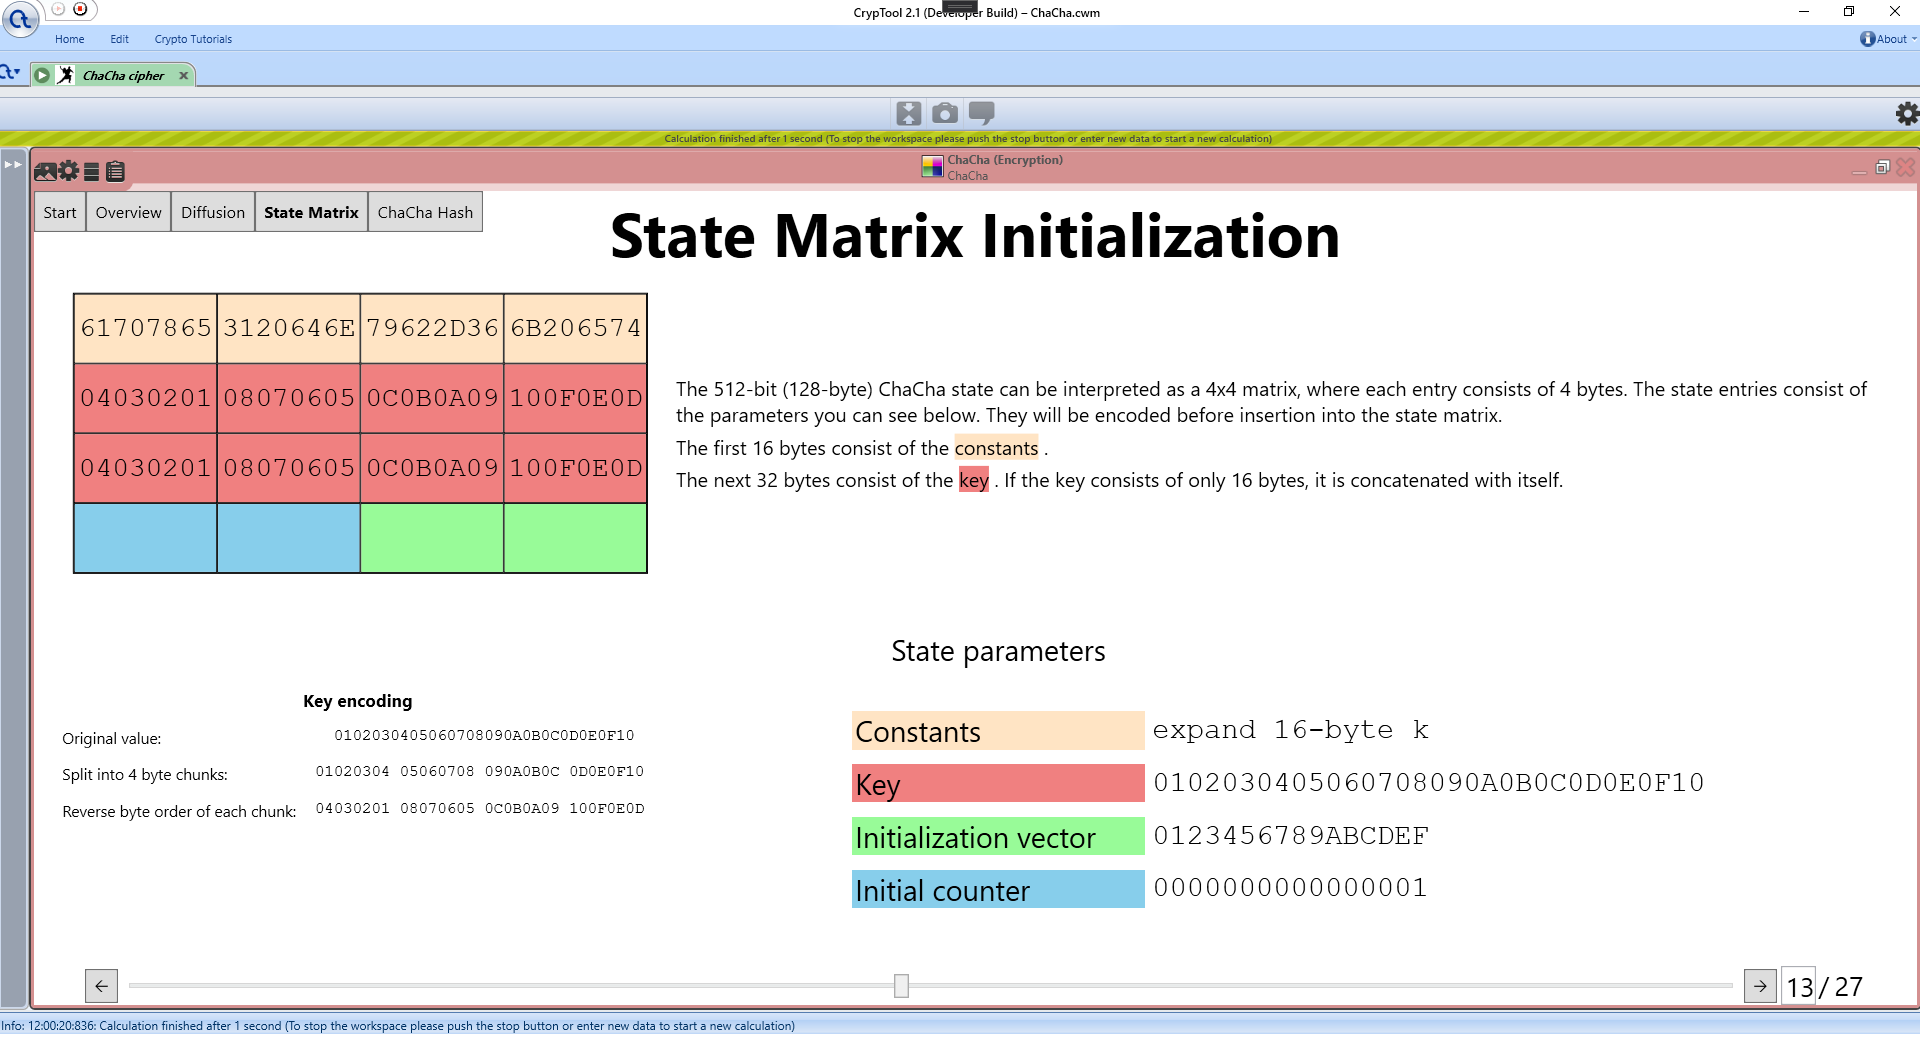
\includegraphics[width=\textwidth]{figures/ct2/state-matrix/2-state-matrix-key.png}
  \caption{Key encoding}
  \label{fig:statematrix.encoding.key}
\end{subfigure}
\end{figure}
\begin{figure}
\ContinuedFloat
\begin{subfigure}{\textwidth}
  \centering
  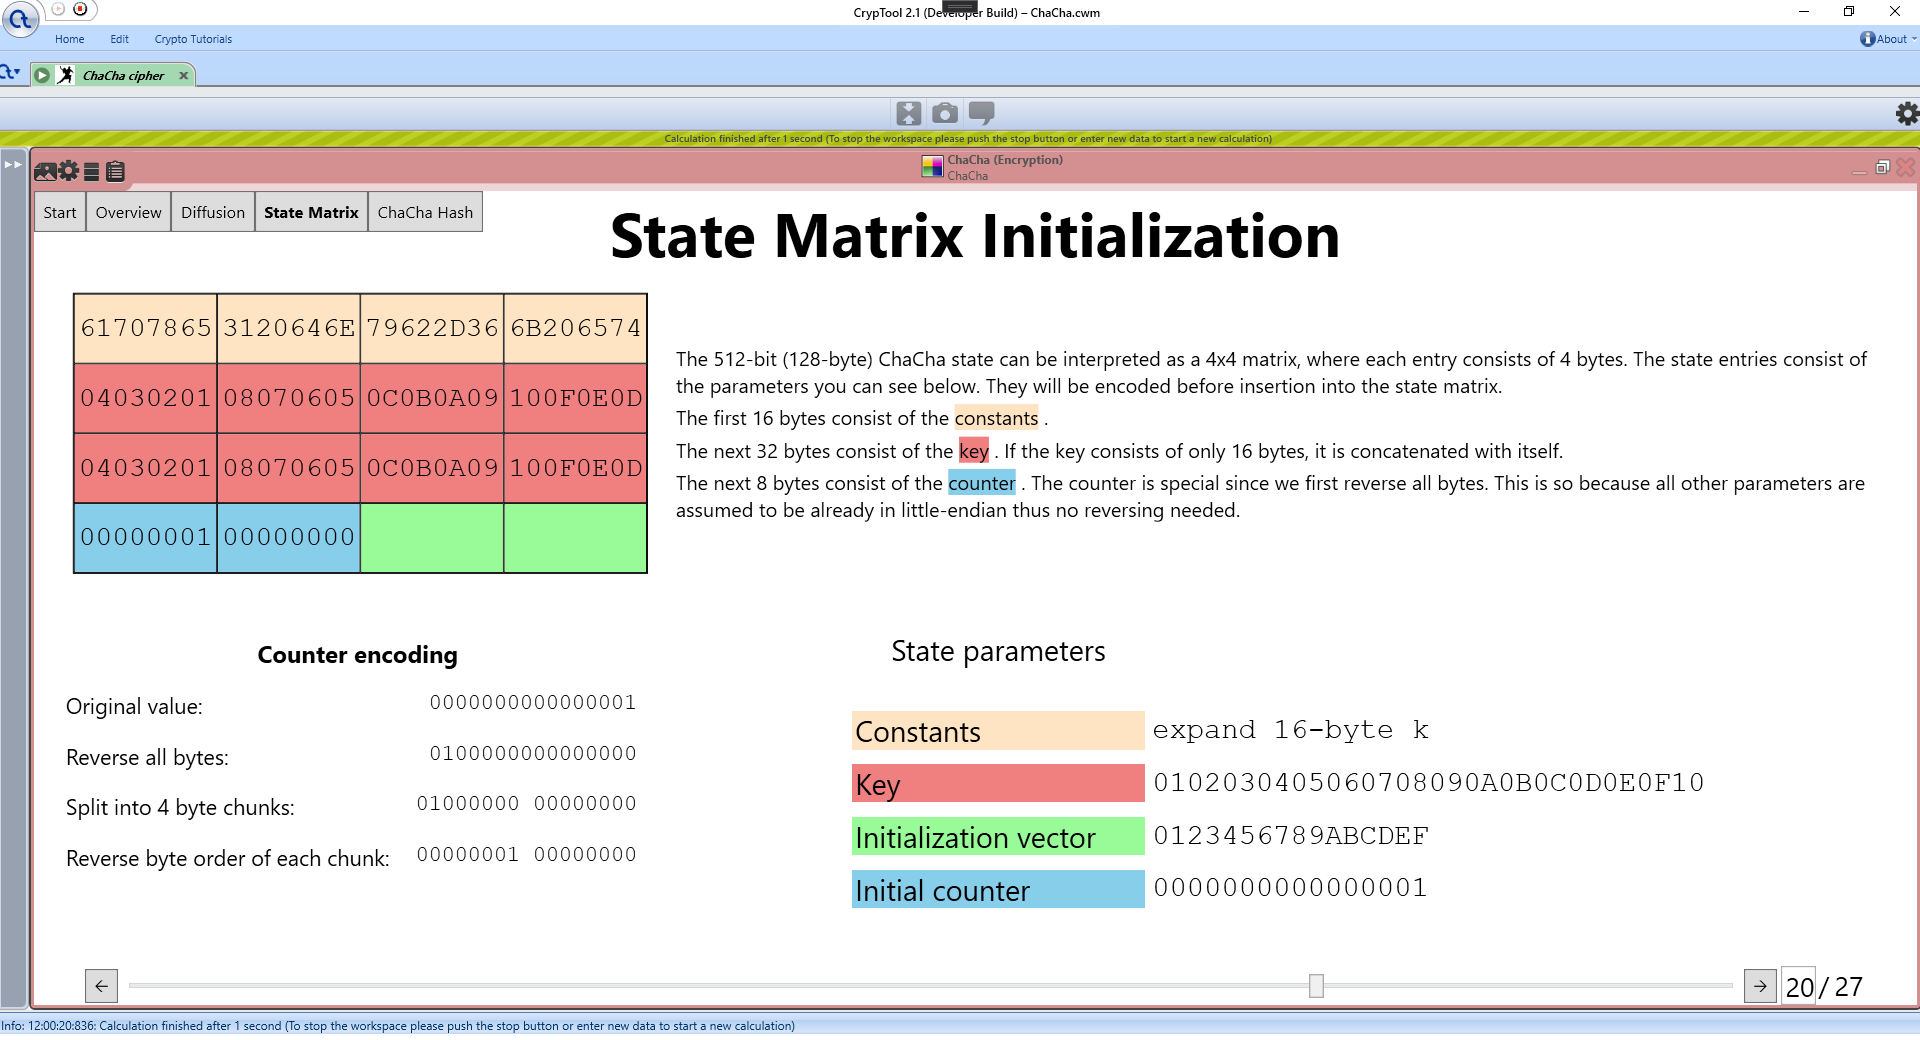
\includegraphics[width=\textwidth]{figures/ct2/state-matrix/3-state-matrix-counter.png}
  \caption{Counter encoding}
  \label{fig:statematrix.encoding.counter}
\end{subfigure}
\begin{subfigure}{\textwidth}
  \centering
  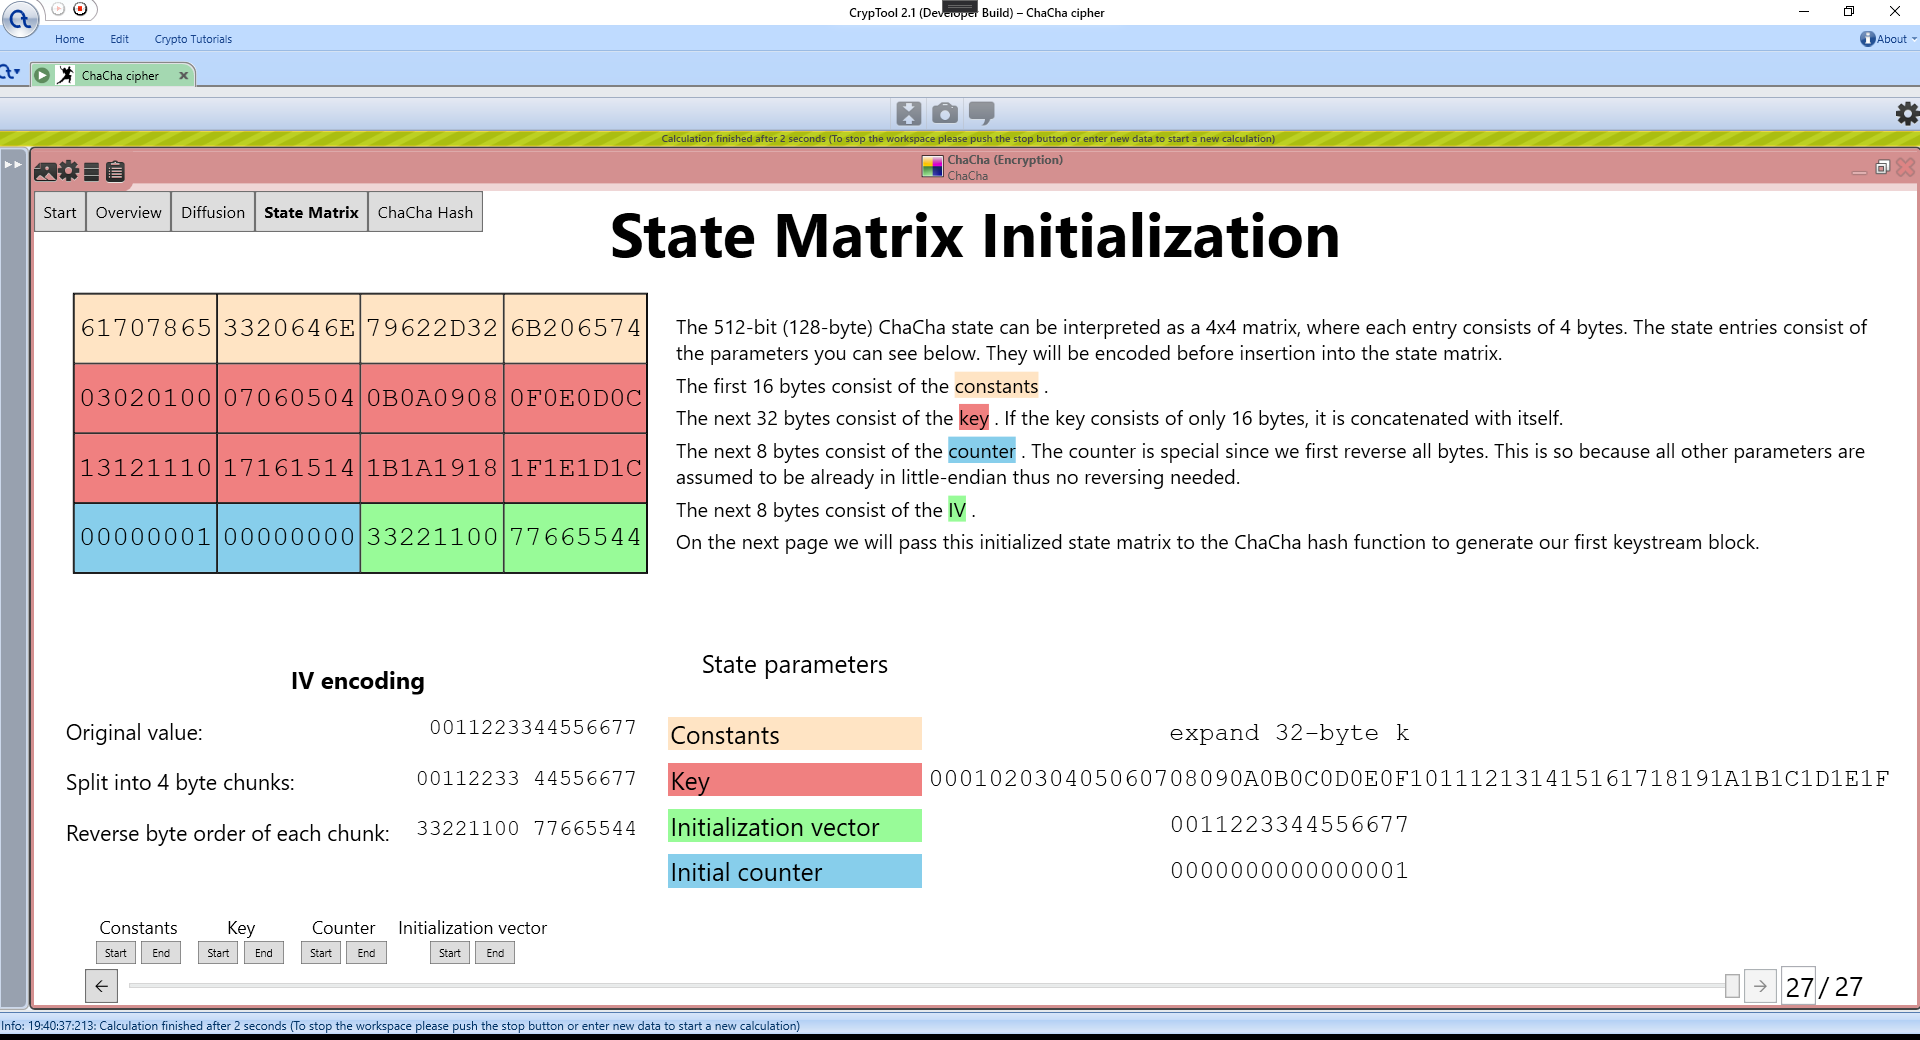
\includegraphics[width=\textwidth]{figures/ct2/state-matrix/4-state-matrix-iv.png}
  \caption{IV encoding}
  \label{fig:statematrix.encoding.iv}
\end{subfigure}
\caption[State Matrix Initialization page]{Encoding of the state parameters on the State Matrix Initialization page}
\label{fig:statematrix.encoding}
\end{figure}

\FloatBarrier

\begin{figure}[h]
\centering
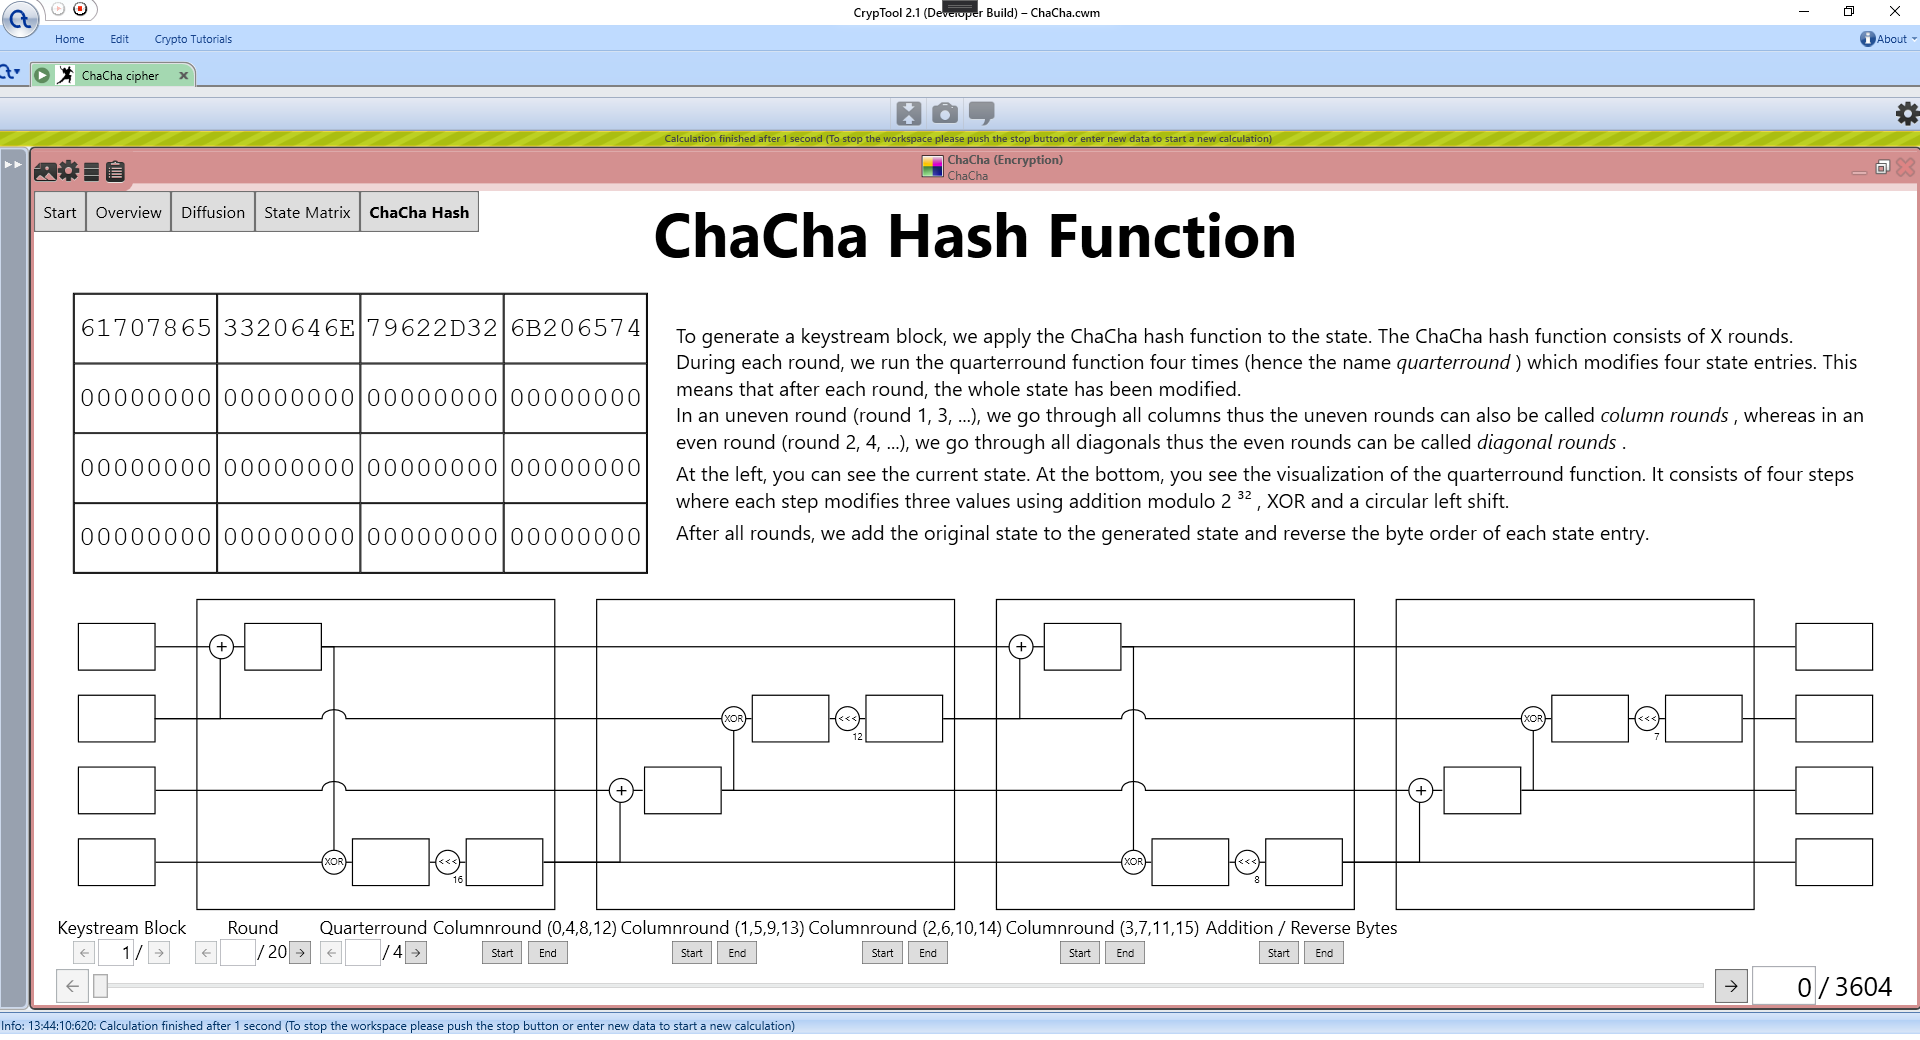
\includegraphics[width=\textwidth]{figures/ct2/all-pages/5-chachahash.png}
\caption{ChaCha Hash Function page in its initial state}
\label{fig:chachahashpage}
\end{figure}

\subsubsection{ChaCha Hash Function page}

The ChaCha Hash Function page (Figure \ref{fig:chachahashpage}) visualizes the generation of a keystream block by using two kind of visualizations: The quarter-round visualization (Figure \ref{fig:chachahash.mid.qr}) and the addition / reverse bytes step visualization at the end of the hash function (Figure \ref{fig:chachahash.end}).

\begin{figure}
  \centering
  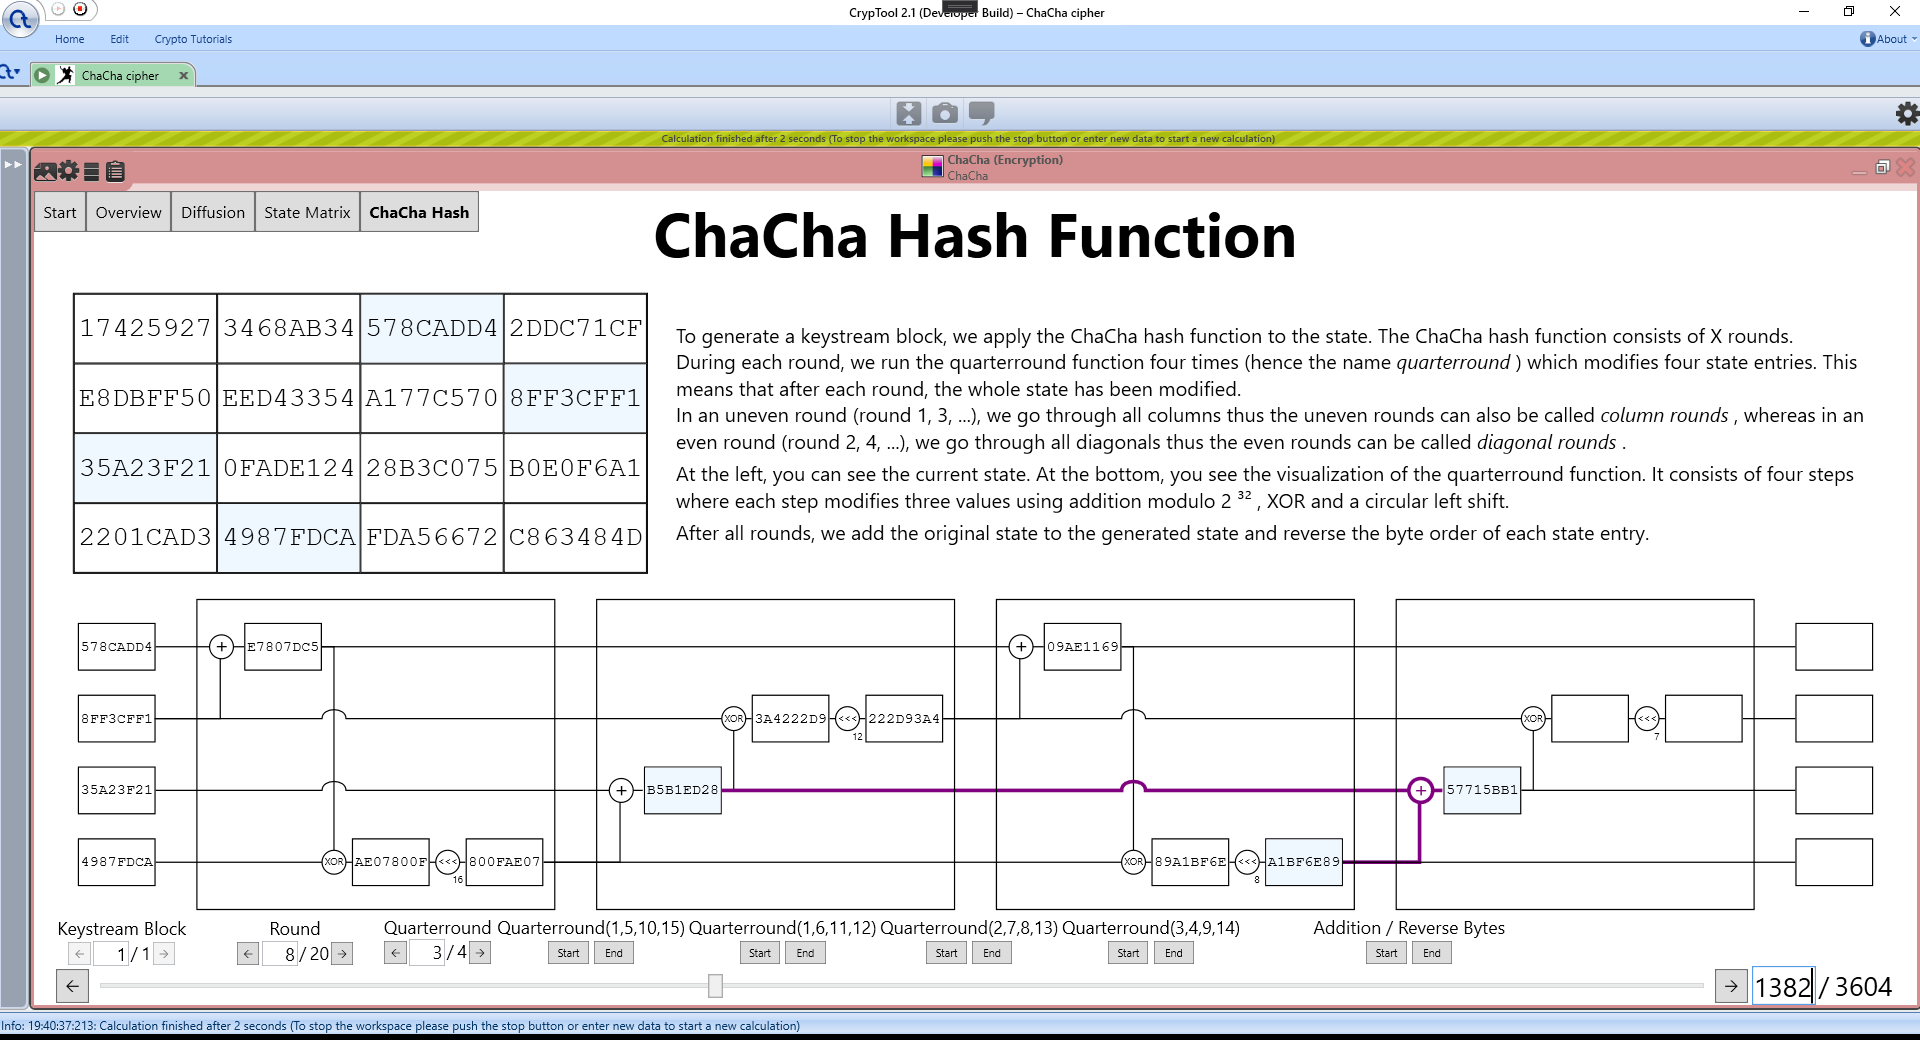
\includegraphics[width=\textwidth]{figures/ct2/chachahash/chachahash-mid-qr.png}
  \caption{Quarter-round visualization}
  \label{fig:chachahash.mid.qr}
\end{figure}

At the top of the page, you can see the current state together with a description about the ChaCha hash function. At the bottom, if we are still in the ChaCha hash function loop (as described in Section \ref{sec:chacha.hash}), you can see the visualization of the quarter-rounds (Figure \ref{fig:chachahash.mid.qr}). The quarter-round visualization is split into four cells on either side and four boxes in the middle. The boxes on the two ends contain the four input and output values of the quarter-round. The boxes in the middle visualize one quarter-round step as was described in Section \ref{sec:chacha.qr}.

A circuit diagram was used to visualize the quarter-round function similar to the one found in the ChaCha section on the Wikipedia page about Salsa20 (see Figure \ref{fig:wiki.qr.circuit}). This way, the intermediate values could just be put on the circuit lines and following along the visualization was very clear because all next steps are already shown.

If we are finished with the loop, we can see the original state at the left, the result of adding the original state with the state after all rounds in the middle, and at the right the result of reversing the byte order of each state entry of the state in the middle (Figure \ref{fig:chachahash.end}). This is the final state and thus one 512-bit block inside the keystream with which the input message is later XOR'ed .

\begin{figure}
\centering
\begin{subfigure}[t]{0.5\textwidth}
  \centering
  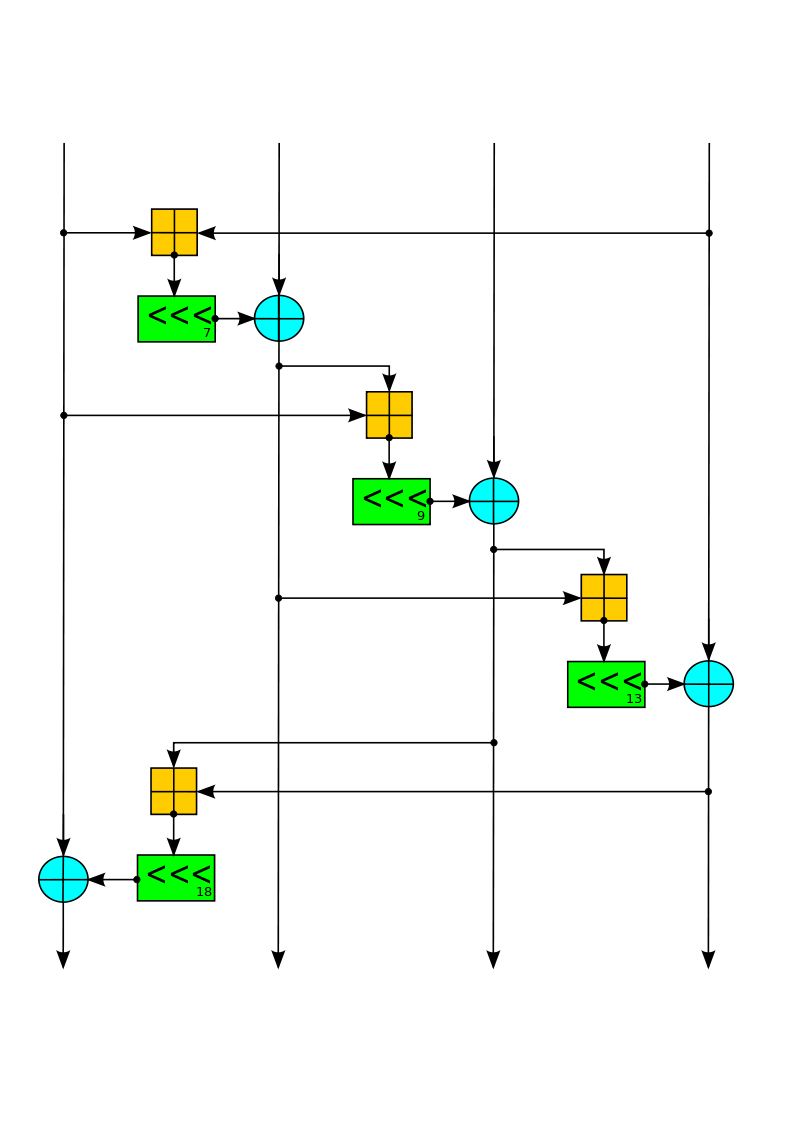
\includegraphics[width=\textwidth]{figures/wiki-qr-circuit/salsa-wiki-qr-circuit.png}
  \caption[Salsa quarter-round circuit diagram]{Salsa quarter-round circuit diagram}
  \label{fig:wiki.qr.circuit.salsa}
\end{subfigure}%
\begin{subfigure}[t]{0.5\textwidth}
  \centering
  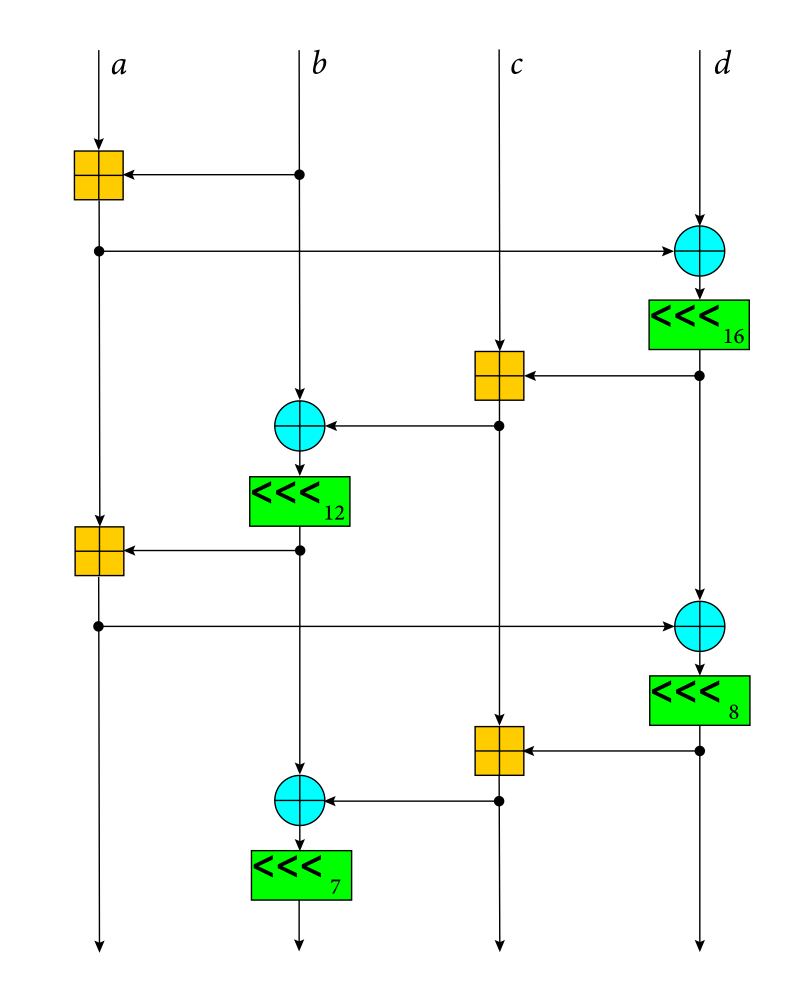
\includegraphics[width=\textwidth]{figures/wiki-qr-circuit/chacha-wiki-qr-circuit.png}
  \caption[ChaCha quarter-round circuit diagram]{ChaCha quarter-round circuit diagram}
  \label{fig:wiki.qr.circuit.chacha}
\end{subfigure}
\caption[Quarter-round circuit diagram]{Quarter-round circuit diagram\\
Source:\\
(a): \url{https://en.wikipedia.org/wiki/Salsa20}\\
(b): \url{https://en.wikipedia.org/wiki/Salsa20\#ChaCha_variant}}
\label{fig:wiki.qr.circuit}
\centering
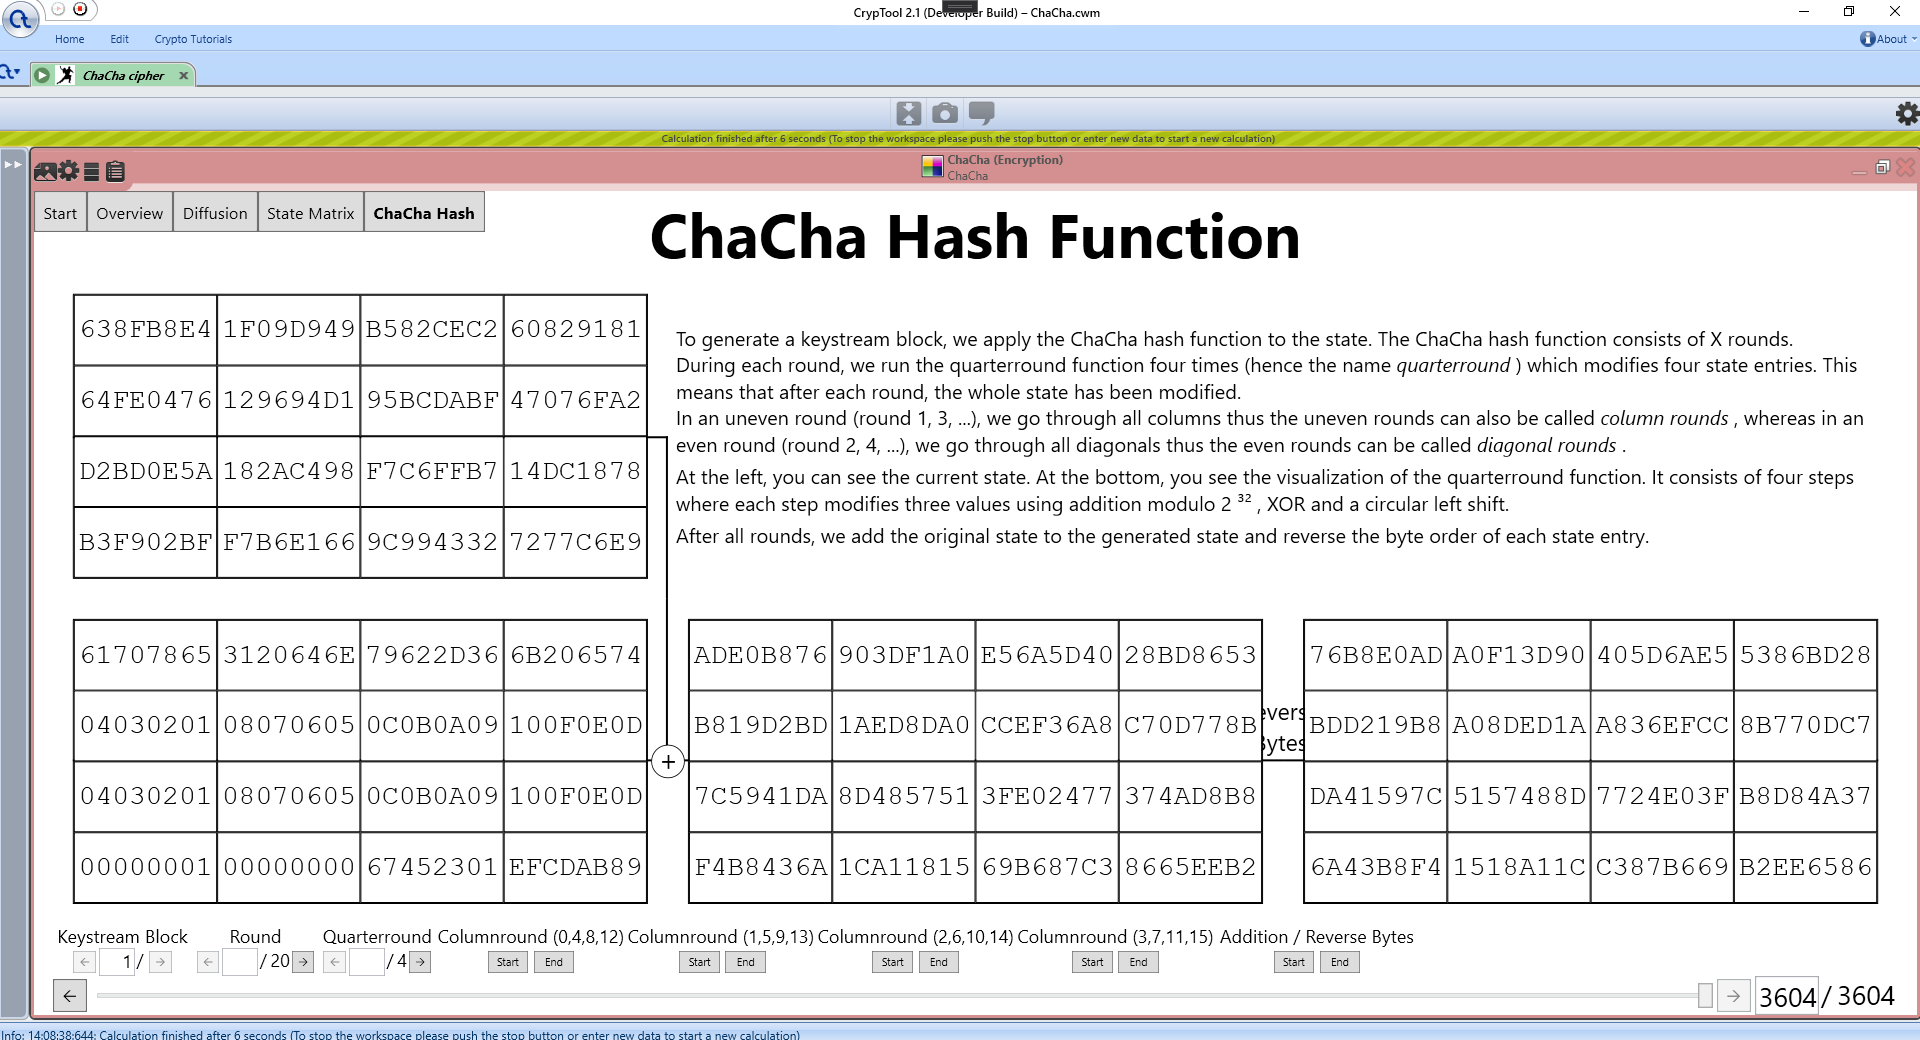
\includegraphics[width=\textwidth]{figures/ct2/chachahash/chachahash-end.png}
\caption{Addition and little-endian step visualization}
\label{fig:chachahash.end}
\end{figure}

Below the visualization and just above the slider for the page actions is another navigation bar. This helps the user to quickly navigate through the ChaCha hash function. He can use the arrow buttons to traverse through the keystream blocks, rounds or quarter-rounds or enter a number to directly go to a specific step. \\
Since entering a number into each text input or using the arrows will only bring the user to the start of each step, he can use the buttons to the right of the quarter-round input to jump to the end of specific quarter-rounds of the current round. \\
These buttons also show the state indices that will get updated during their quarter-round in parentheses. Since column and diagonal rounds take turns, these labels show the state indices according to the current round.

Figure \ref{fig:chachahash.dr} shows exemplary how the page looks like at the end of each quarter-round of a diagonal round. As you can see, the corresponding state entry is highlighted with a light blue background. This light blue background is also used throughout the visualization to catch the user's attention about which UI elements will be updated in the next step.

\pagebreak

Figure \ref{fig:chachahash.mid.qr.diffusion} shows the quarter-round visualization as an example how diffusion is visualized throughout the plug-in. Figure \ref{fig:chachahash.mid.qr.diffusion.both} shows the visualization with the XOR button in the top-right corner not toggled; thus showing the values from both cipher runs whereas Figure \ref{fig:chachahash.mid.qr.diffusion.xor} shows the visualization with the XOR button toggled.

\begin{figure}
\centering
\begin{subfigure}{0.5\textwidth}
  \centering
  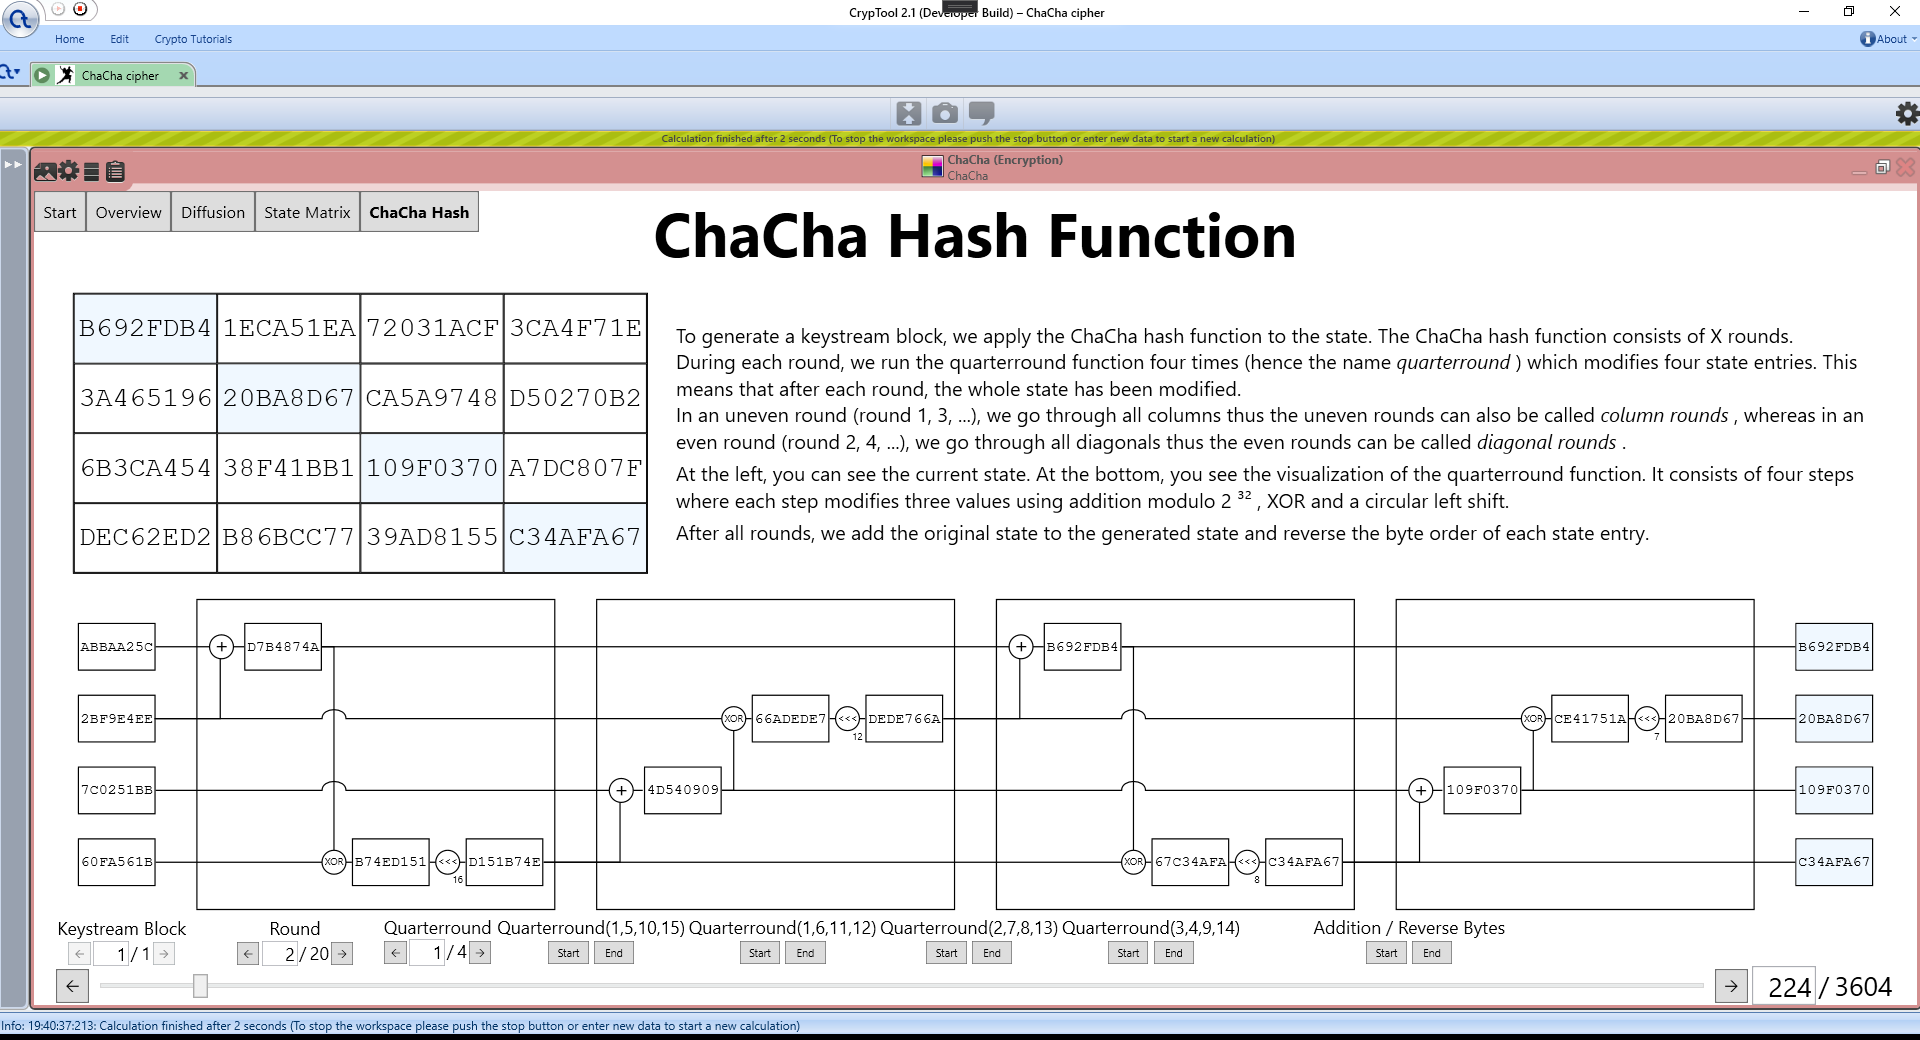
\includegraphics[width=0.99\textwidth]{figures/ct2/chachahash/chachahash-dr1-end.png}
  \caption{End of first quarter-round (diagonal round)}
  \label{fig:chachahash.dr.1}
\end{subfigure}%
\begin{subfigure}{0.5\textwidth}
  \centering
  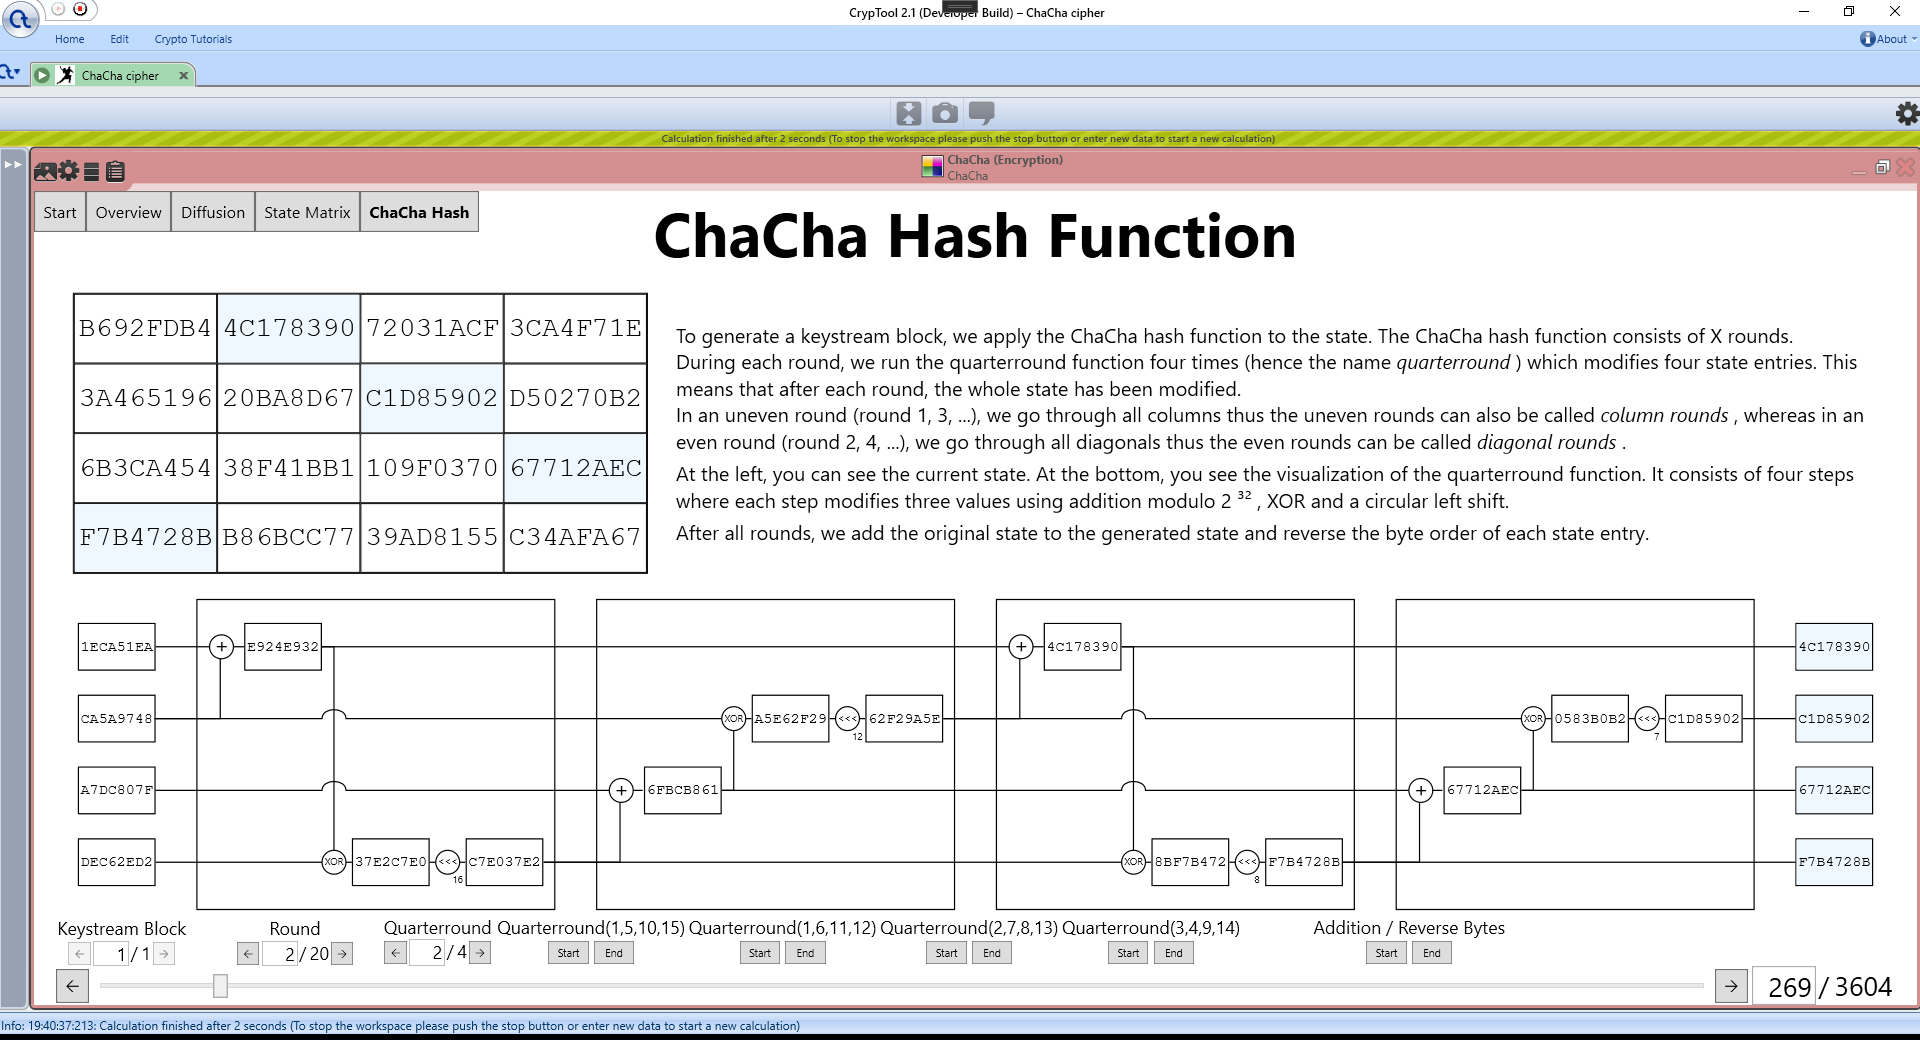
\includegraphics[width=0.99\textwidth]{figures/ct2/chachahash/chachahash-dr2-end.png}
  \caption{End of second quarter-round (diagonal round)}
  \label{fig:chachahash.dr.2}
\end{subfigure}
\begin{subfigure}{0.5\textwidth}
  \centering
  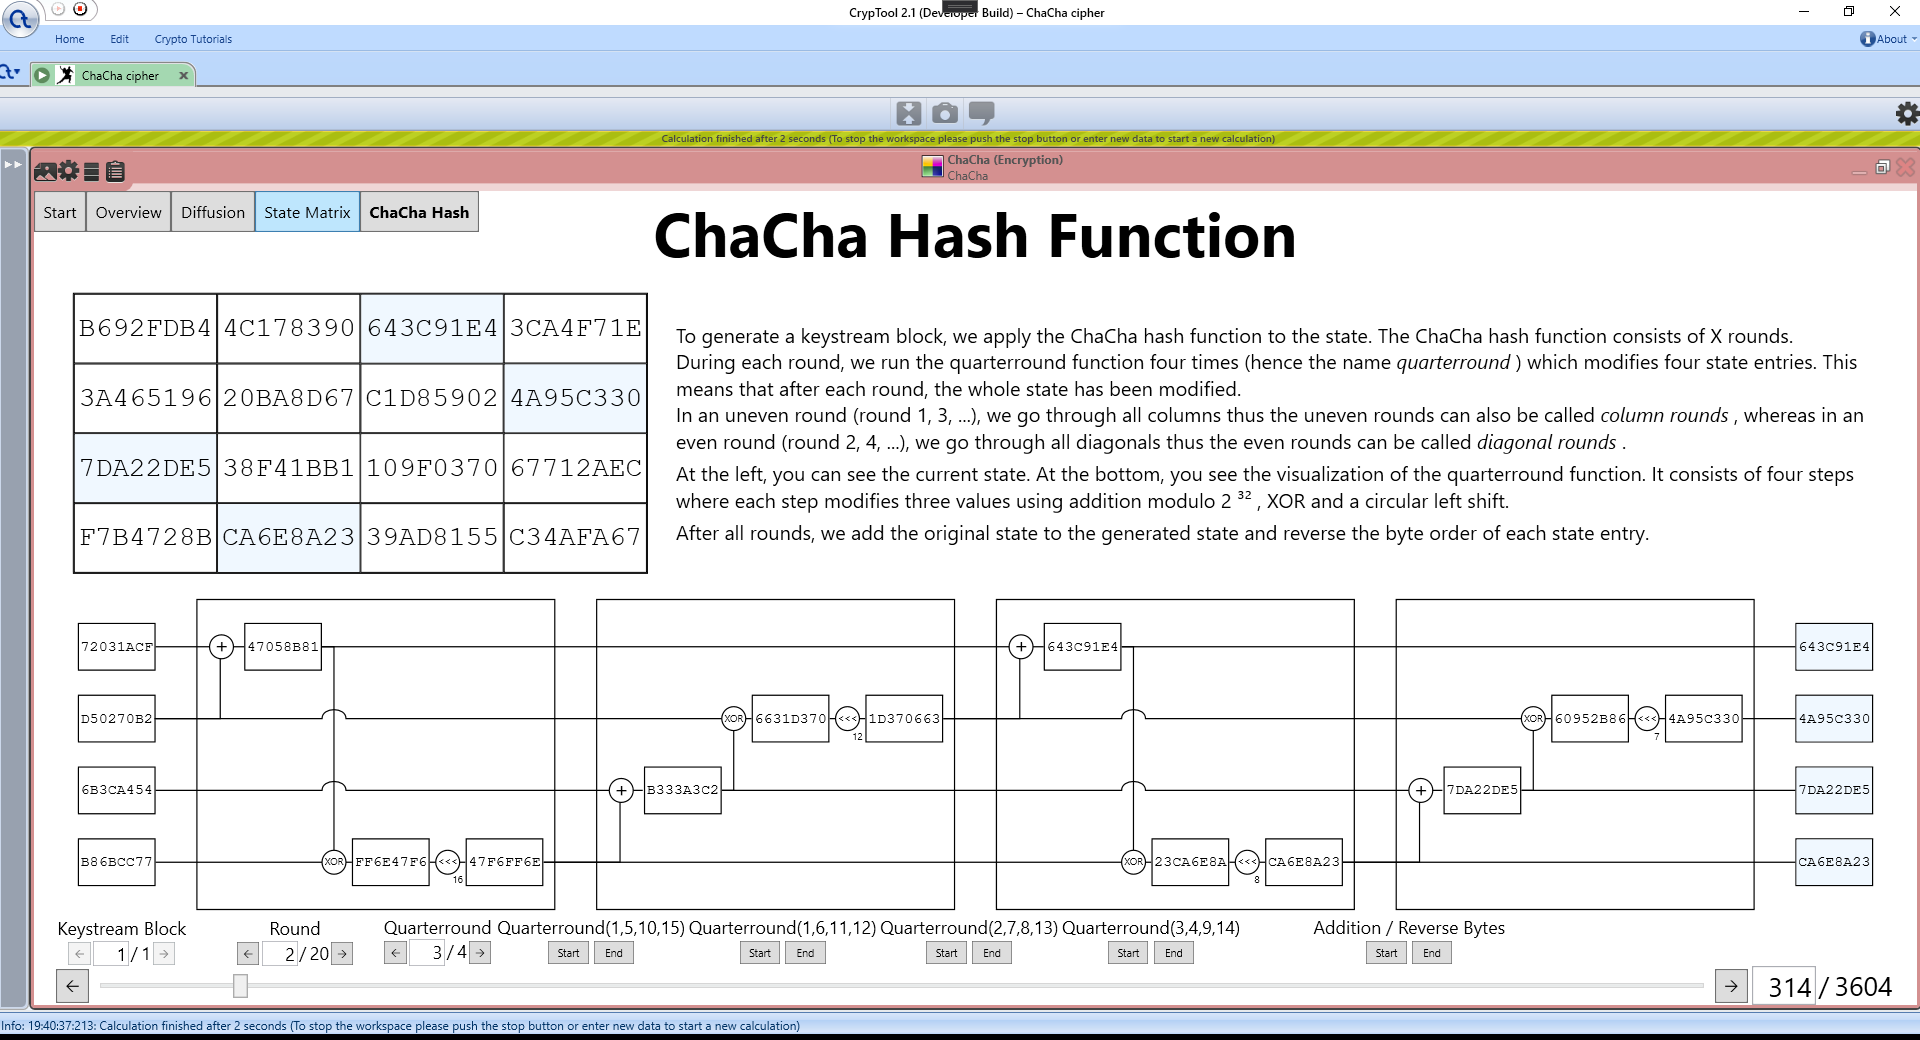
\includegraphics[width=0.99\textwidth]{figures/ct2/chachahash/chachahash-dr3-end.png}
  \caption{End of third quarter-round (diagonal round)}
  \label{fig:chachahash.dr.3}
\end{subfigure}%
\begin{subfigure}{0.5\textwidth}
  \centering
  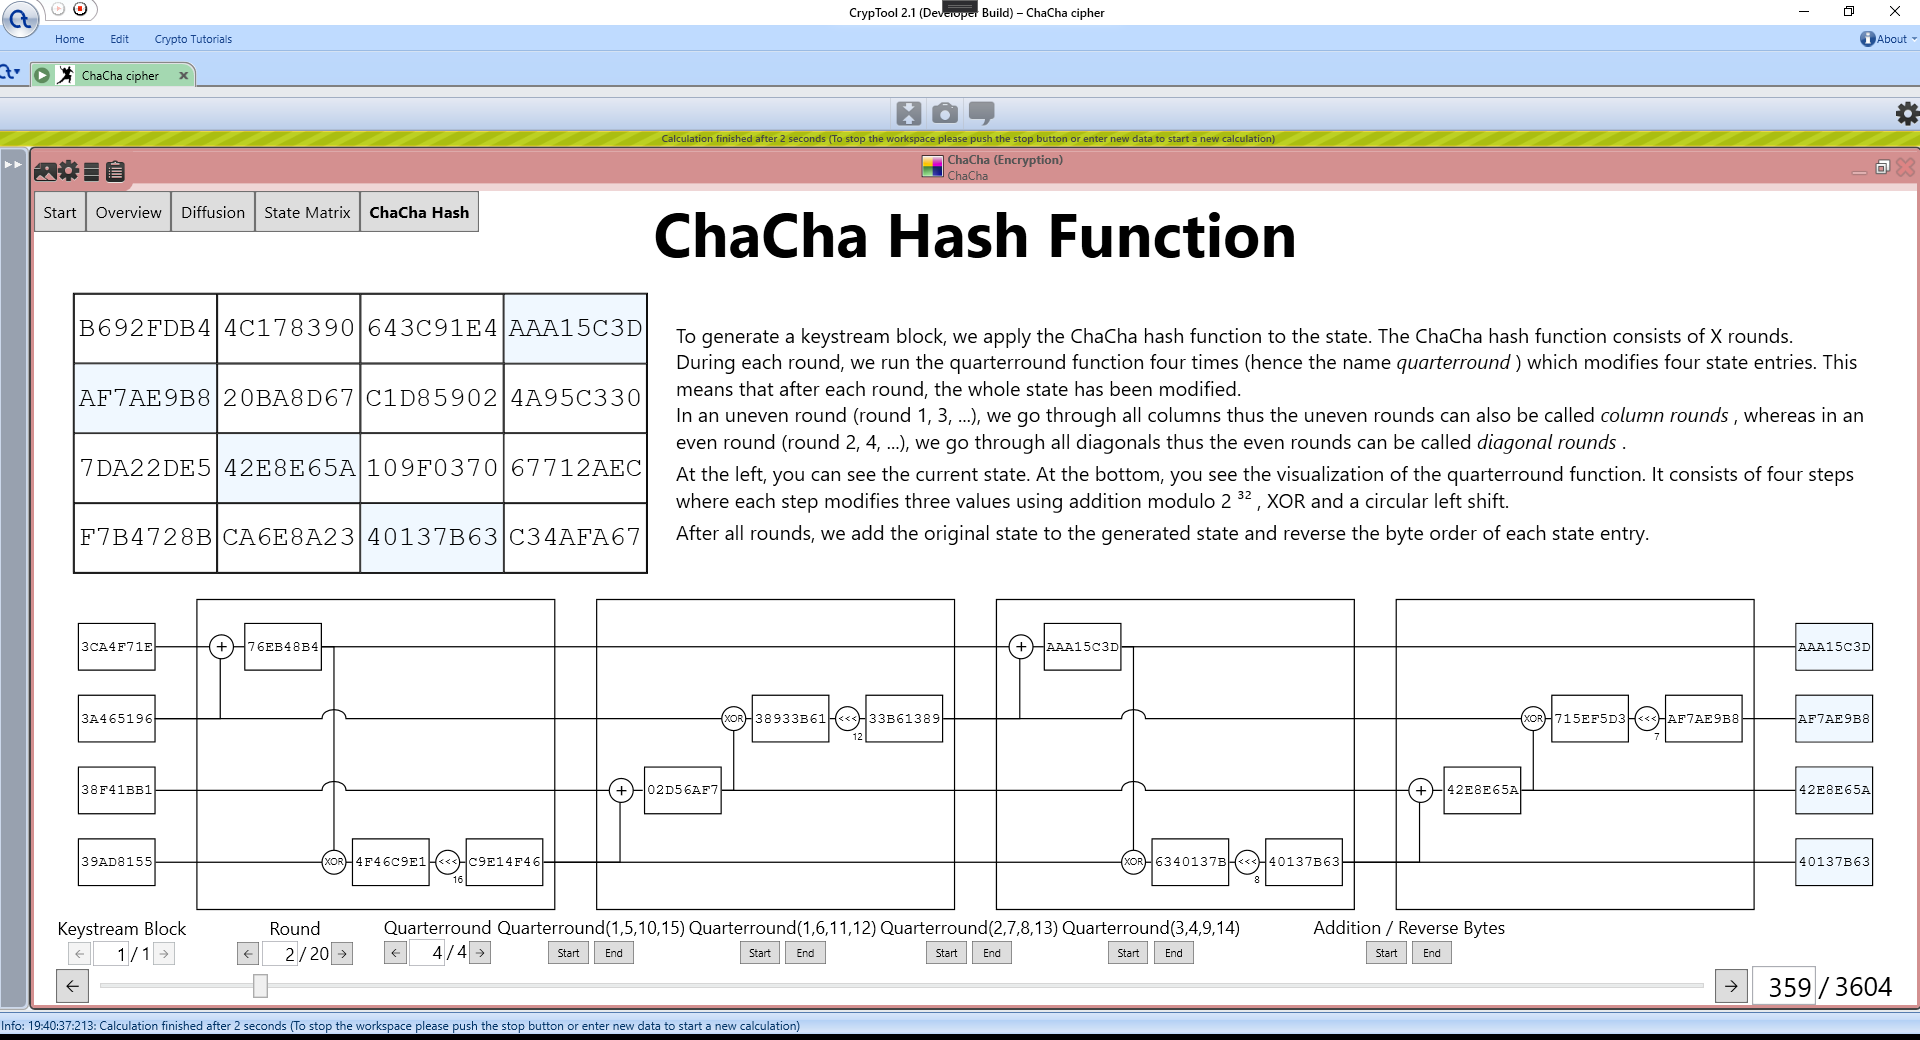
\includegraphics[width=0.99\textwidth]{figures/ct2/chachahash/chachahash-dr4-end.png}
  \caption{End of fourth quarter-round (diagonal round)}
  \label{fig:chachahash.dr.4}
\end{subfigure}
\caption[End of diagonal rounds]{End of each quarterround execution of a diagonal round}
\label{fig:chachahash.dr}
\end{figure}

\begin{figure}
\begin{subfigure}[t]{\textwidth}
  \centering
  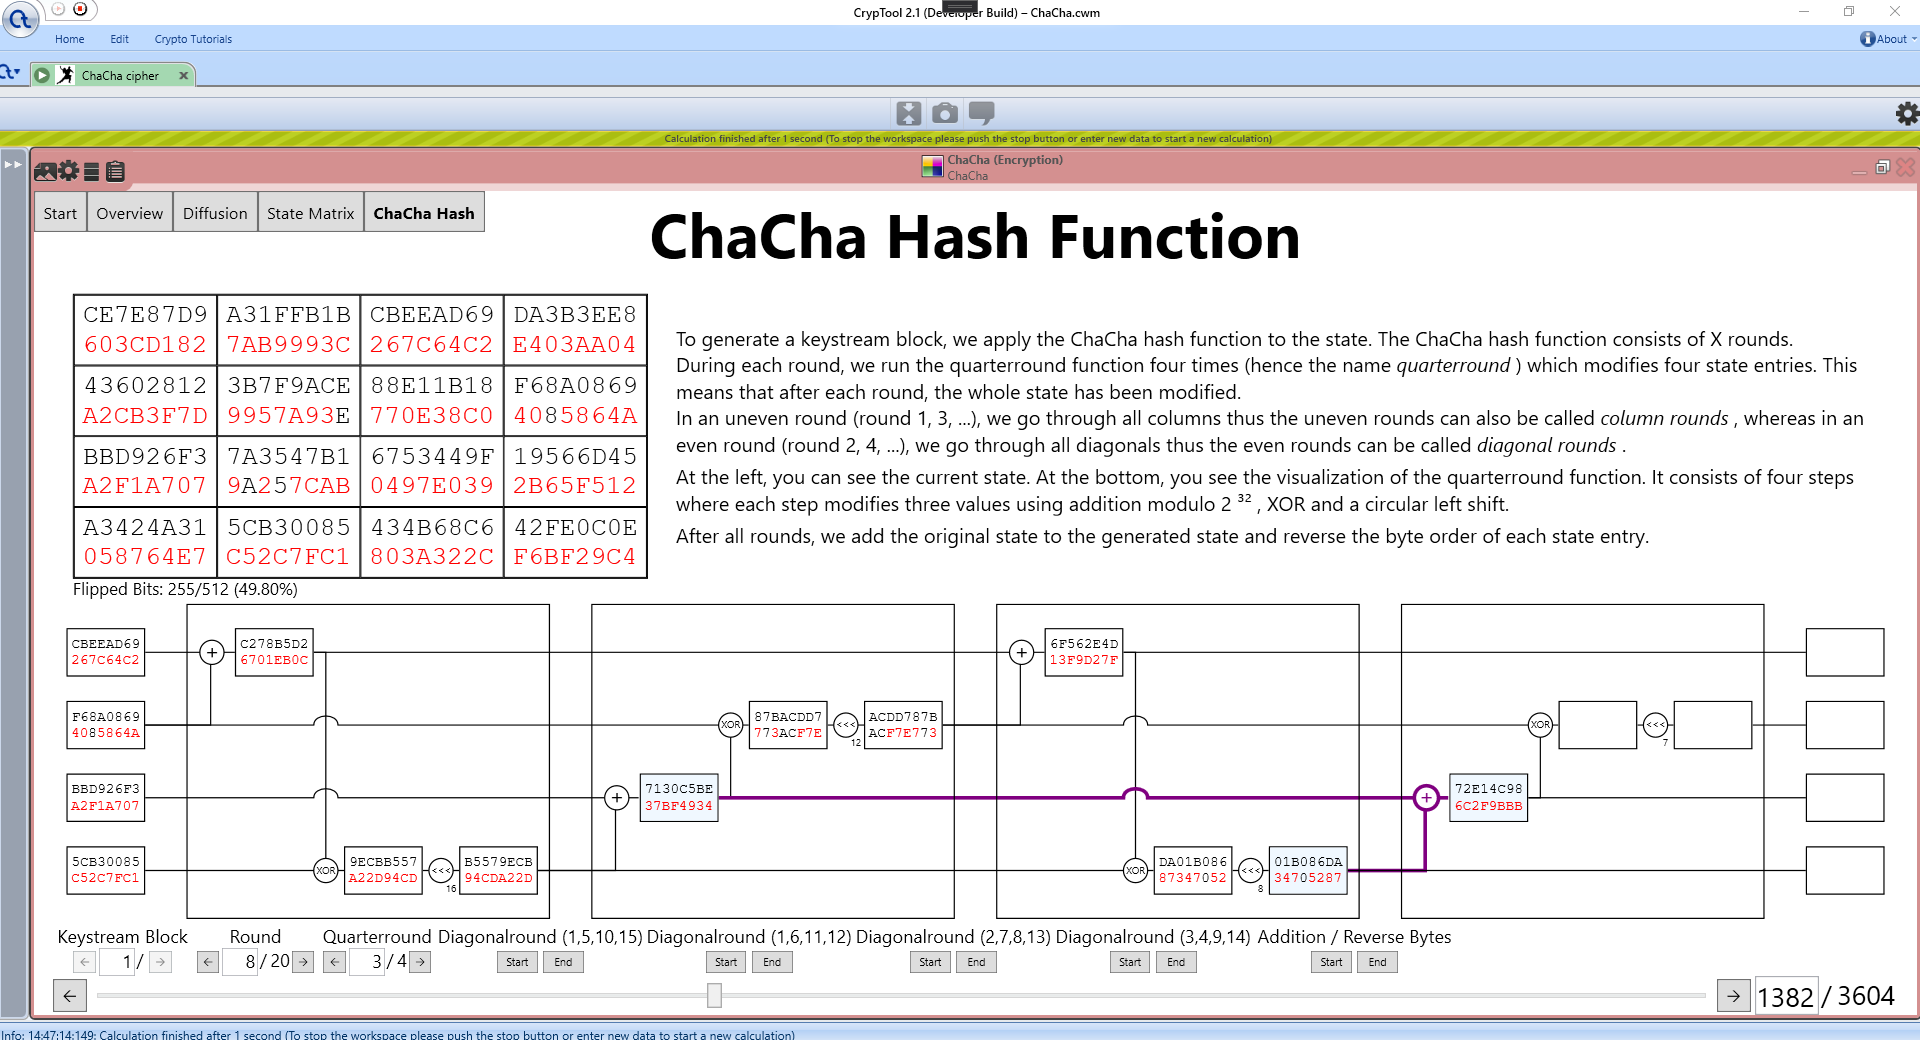
\includegraphics[width=\textwidth]{figures/ct2/chachahash/chachahash-mid-qr-diffusion.png}
  \caption{Quarter-round visualization with diffusion (showing both values)}
  \label{fig:chachahash.mid.qr.diffusion.both}
\end{subfigure}
\begin{subfigure}[t]{\textwidth}
  \centering
  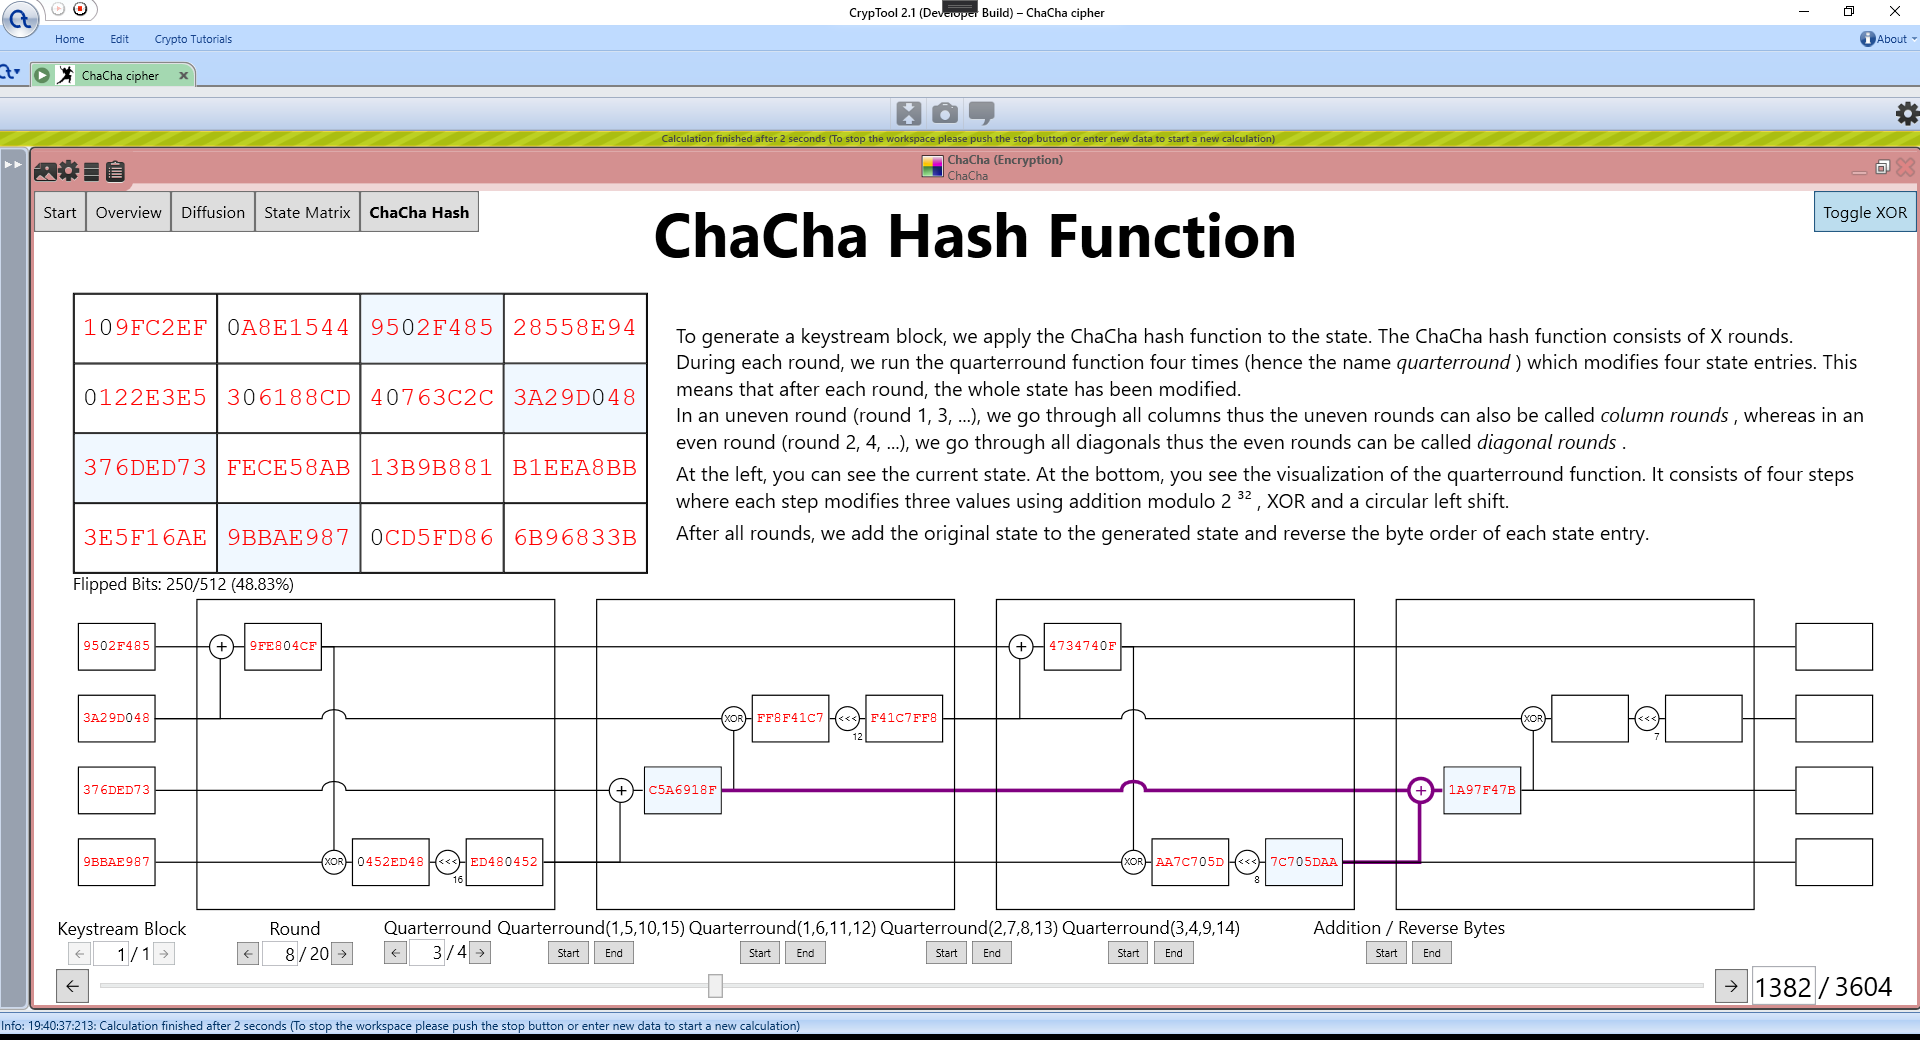
\includegraphics[width=\textwidth]{figures/ct2/chachahash/chachahash-mid-qr-diffusion-xor.png}
  \caption{Quarter-round visualization with diffusion (showing XOR)}
  \label{fig:chachahash.mid.qr.diffusion.xor}
\end{subfigure}
\caption{Quarter-round visualization with diffusion}
\label{fig:chachahash.mid.qr.diffusion}
\end{figure}


%%%%%%%%%%%%%%%%%%%%%%%%%%%%%%%%%%%%%%%%%%%%%%%%%%%%%%%%%%%%%%%%%%%%%%%%

\FloatBarrier
\subsection{Architecture}
\label{sec:Architecture}

This section will go more into detail how the software was layed out.

\noindent
The software architecture, which was written using WPF (Windows Presentation Foundation), XAML and C\#7.0, can be split into two parts. \\
The first part is about the MVVM (Model-View-ViewModel) architecture to create the user interface which was explained in the previous section, using WPF built-in tools such as data binding, templates, converters and validation rules. \\
The second part is about the action navigation system which plays a huge role regarding performance. It powers the slider and buttons in the bottom row of each page which has actions. The page navigation is handled by the first part because it is very simple and uses MVVM design patterns.

\subsubsection{MVVM architecture}

The architecture was built with the MVVM design pattern in mind. MVVM stands for Model, View and View Model. As the name suggest, MVVM is all about separating the code into three parts: Models, Views and View Models.

Models hold the raw application data. In our case, this would be the classes which hold the values generated by the ChaCha cipher. It should be completely unaware of any view or view Model.

Views define how the data should be presented. They consist mainly of XAML code with as little code-behind as possible. They do not maintain their own state but rather use data binding to synchronize themselves with the data inside view models. Therefore, views are aware of view models and in fact depend on them to show any relevant data.

View models connect the model data with the views. However, they do not directly manipulate the views but just define properties and methods which implement the logic for user interactions. The views then use data binding to be notified about any property changes or call methods if a button is clicked etc. This means that view models should not rely on any code inside a view. This essentially decouples the backend from the frontend.

\begin{figure}
\centering
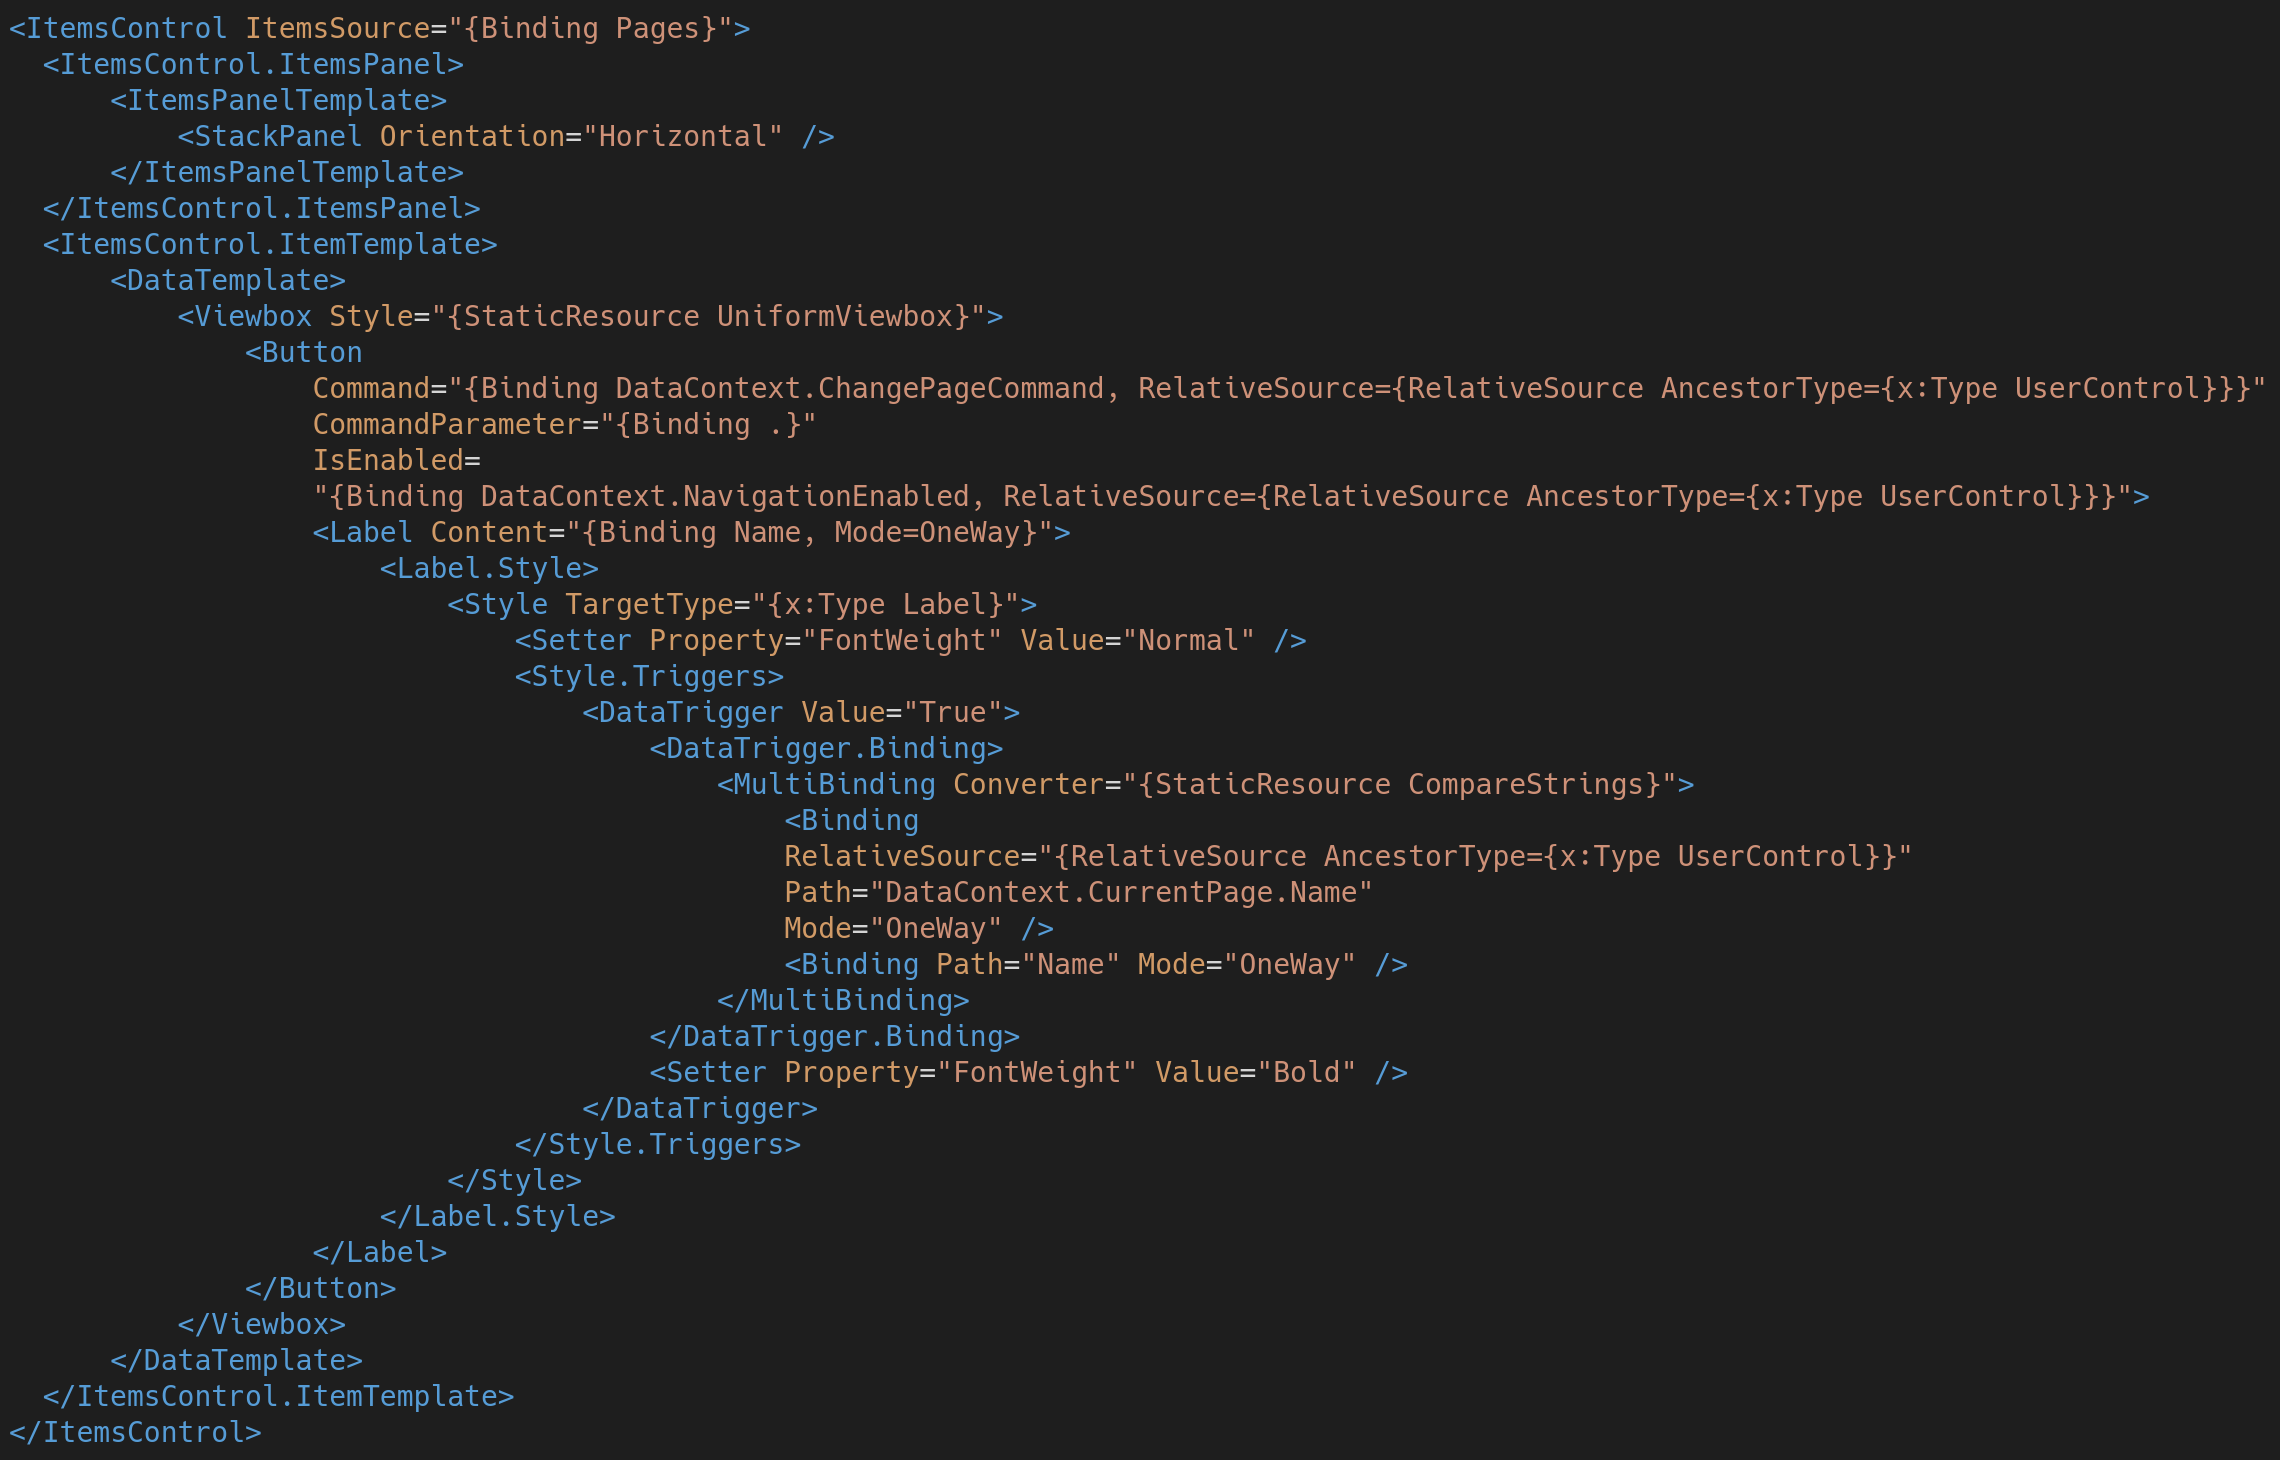
\includegraphics[width=\textwidth]{figures/code/mvvm-arch/page-navigation-template.png}
\caption[Page navigation]{Implementation of page navigation using data binding}
\label{fig:mvvm.pagenavigation}
\end{figure}

In Figure \ref{fig:mvvm.pagenavigation}, an example for how this data binding looks in code is provided. What you see is the view code for the page navigation.

\begin{figure}
\centering
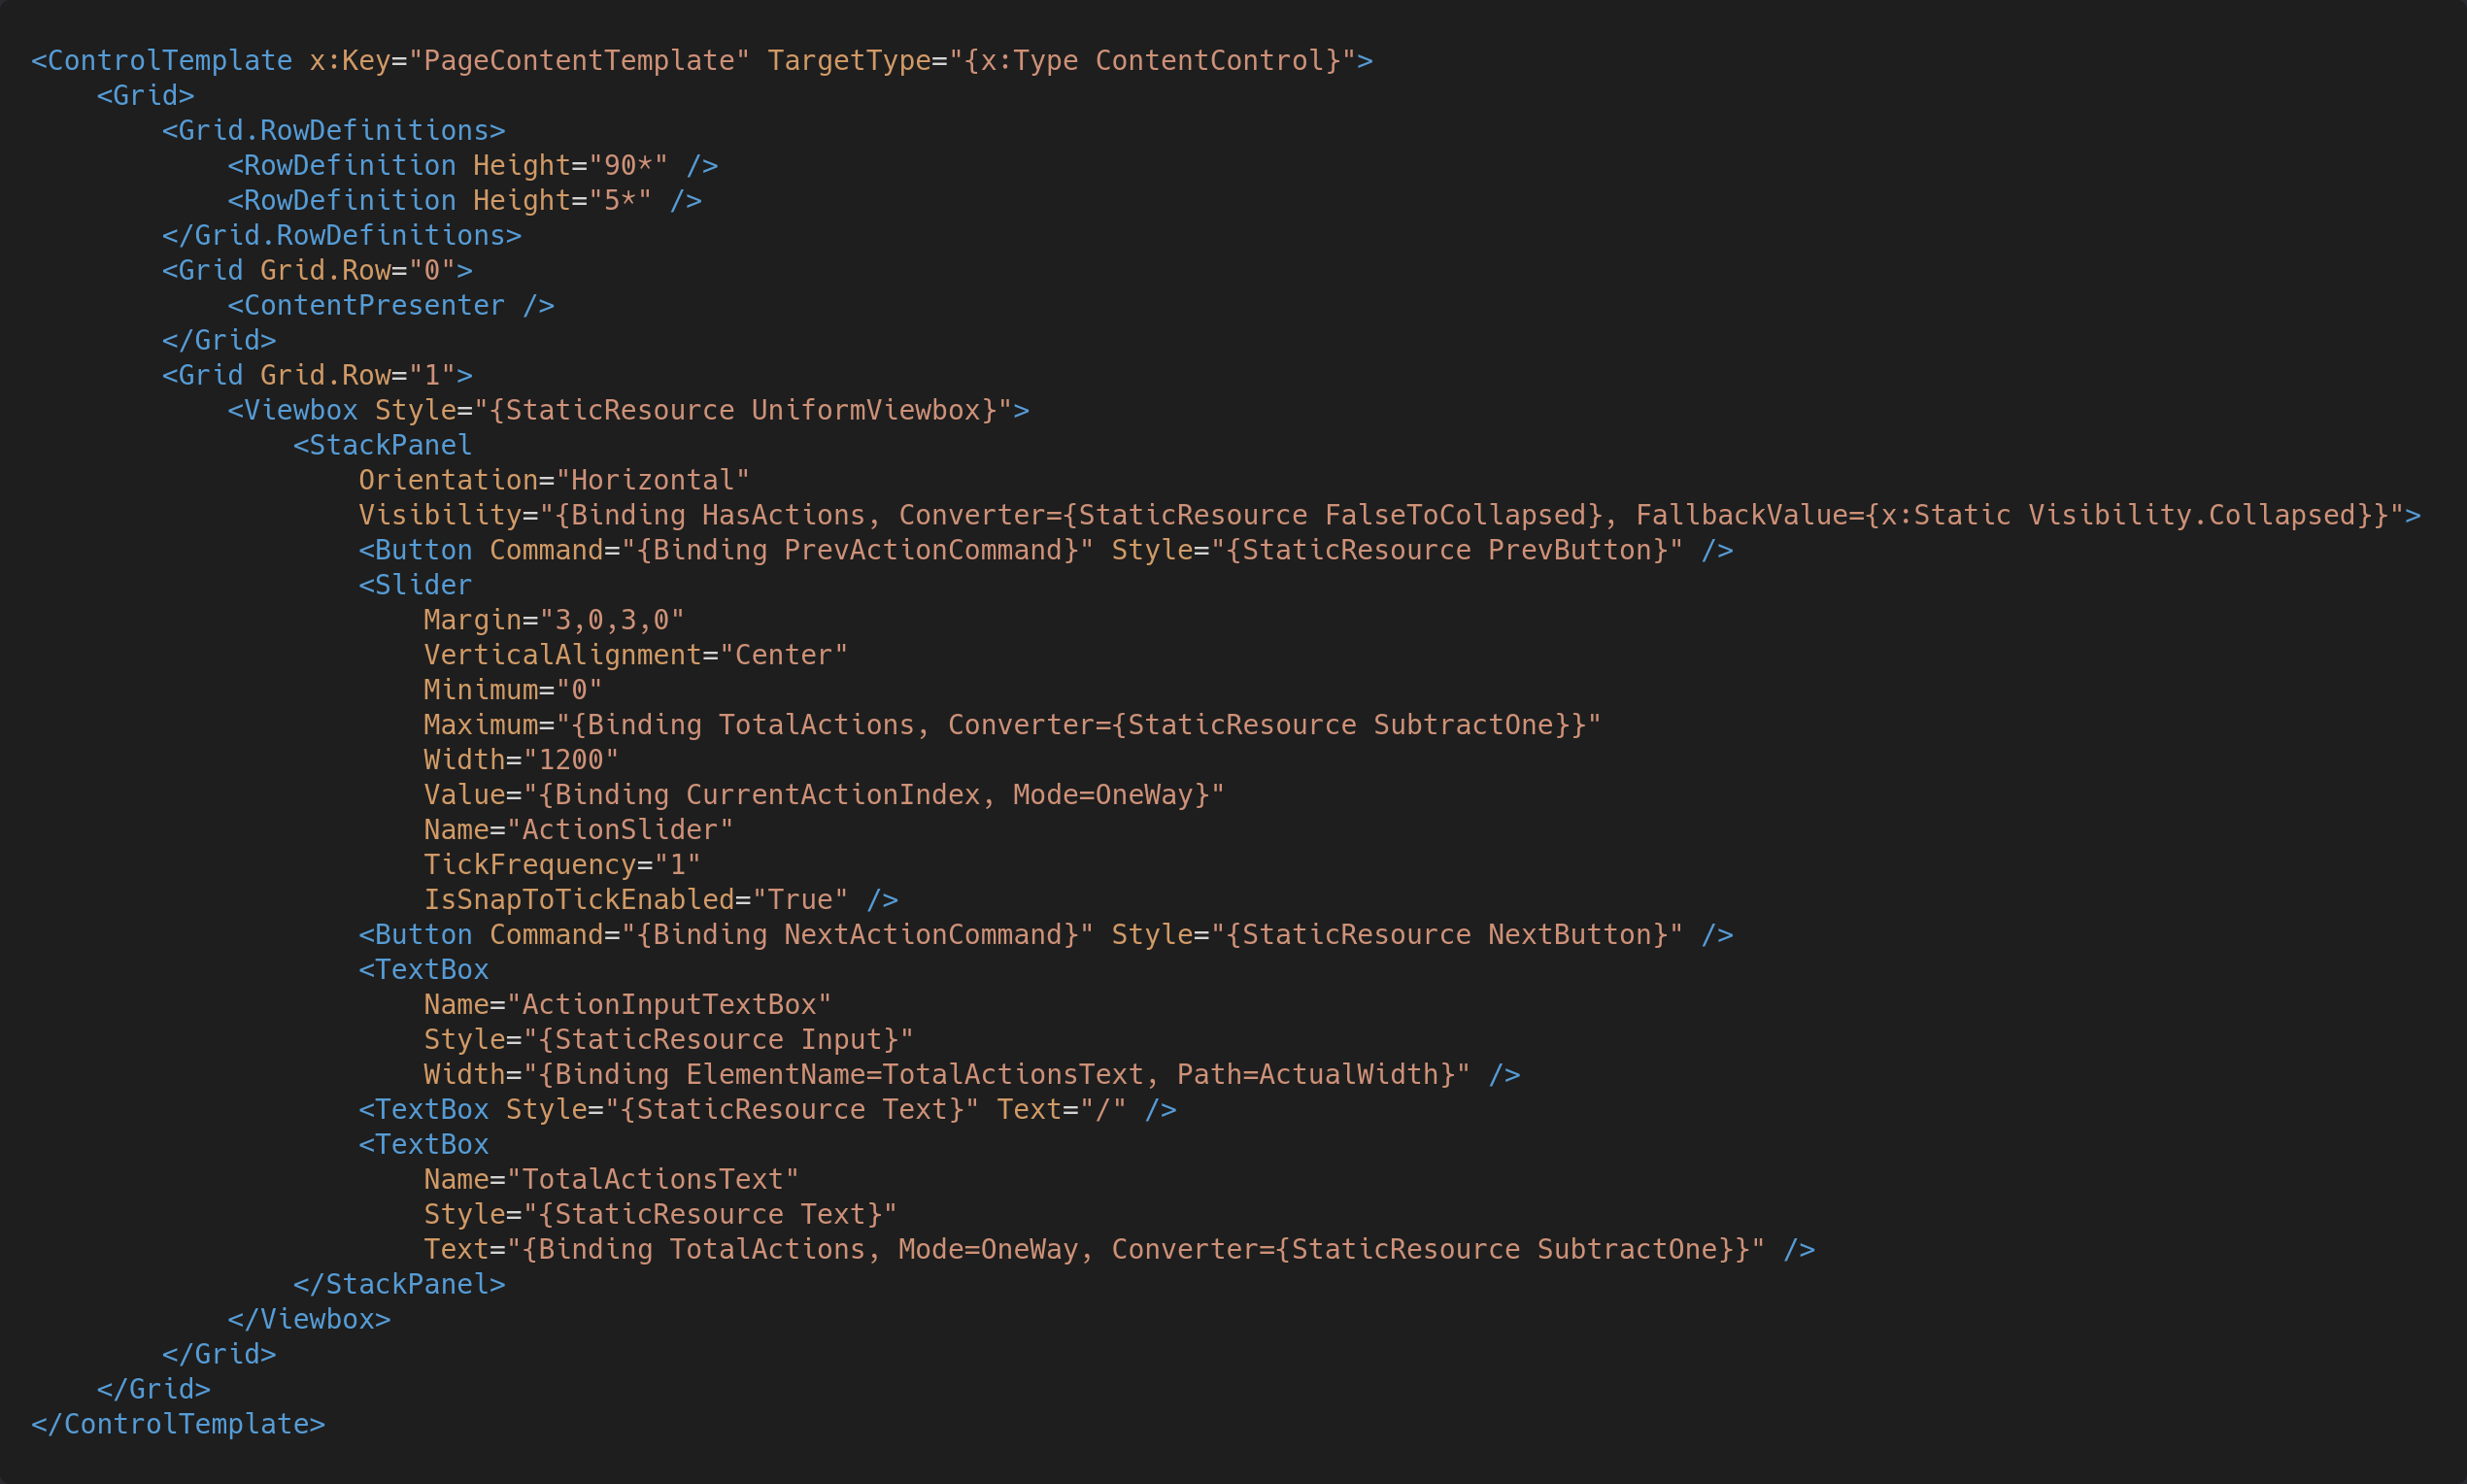
\includegraphics[width=\textwidth]{figures/code/mvvm-arch/action-navigation-template.png}
\caption[Action navigation]{Implementation of action navigation inside a control template}
\label{fig:mvvm.actionnavigation}
\end{figure}

Another technique (that you can also see in the mentioned figure) is the use of templates. Data templates are used to attach views to view models and control templates to implement the general UI structure with the three sections mentioned in Section \ref{sec:userInterface}. This makes it possible to define the UI layout for all pages in one place and also reuse a single implementation of the page and action navigation across all pages. This way, view modifications down the road which applied to all pages were easy and fast. In Figure \ref{fig:mvvm.actionnavigation}, you can see the view implementation of the action navigation bar which is only visible on pages which do have actions.

Since the most interesting part about the MVVM architecture is probably how the diffusion visualization works, this feature will be explained more in-depth in the following.

\subsubsection{Diffusion implementation using MVVM}

If the user enters something into the input fields of the Diffusion page, validation of the input occurs. The validation checks if the input contains only valid hexadecimal characters and if the size is not too large. This is done by using two-way bindings and extending the \texttt{ValidationRule} class which is a built-in module of WPF. Only if the input is valid, the value is saved into a property of the underlying view model. This way, we can be sure that we always have sane data with which we later can execute the cipher with.

Furthermore, converters which are also built into WPF are used to convert data into user-friendly formats. Converters are always attached to bindings, so inside the two-way bindings, byte arrays are converted into hex strings and vice versa using custom converters.

Data binding works by notifying a view if a variable has changed. WPF provides an interface named \texttt{INotifyPropertyChanged} which helps to implement these data binding notifications. It provides a method named \texttt{OnPropertyChanged} and an event named \texttt{PropertyChangedEventHandler} which must be called with the name of the variable to raise such an notification. The data binding system then updates the variables in the view.

\begin{figure}[!hbt]
\centering
\begin{subfigure}[t]{0.6\textwidth}
\centering
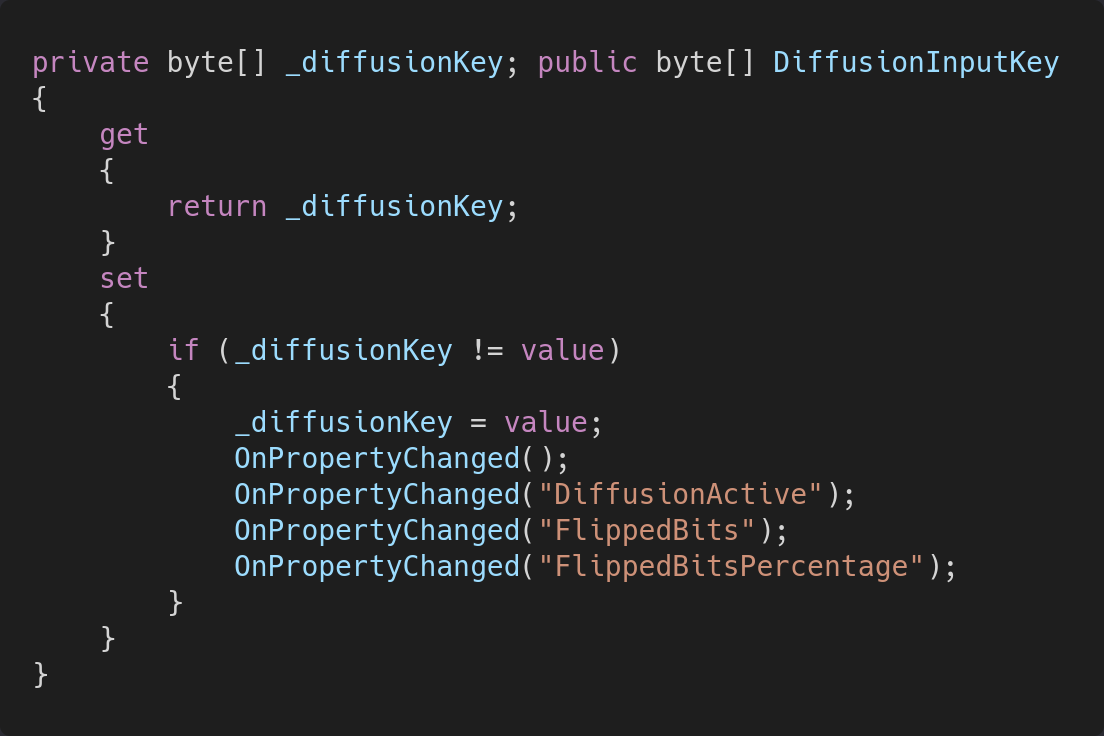
\includegraphics[width=\textwidth]{figures/code/mvvm-arch/onpropertychanged.png}
\caption{Data binding notification in the setter of \texttt{DiffusionInputKey}}
\label{fig:mvvm.onpropertychanged}
\end{subfigure}
\begin{subfigure}[t]{\textwidth}
\centering
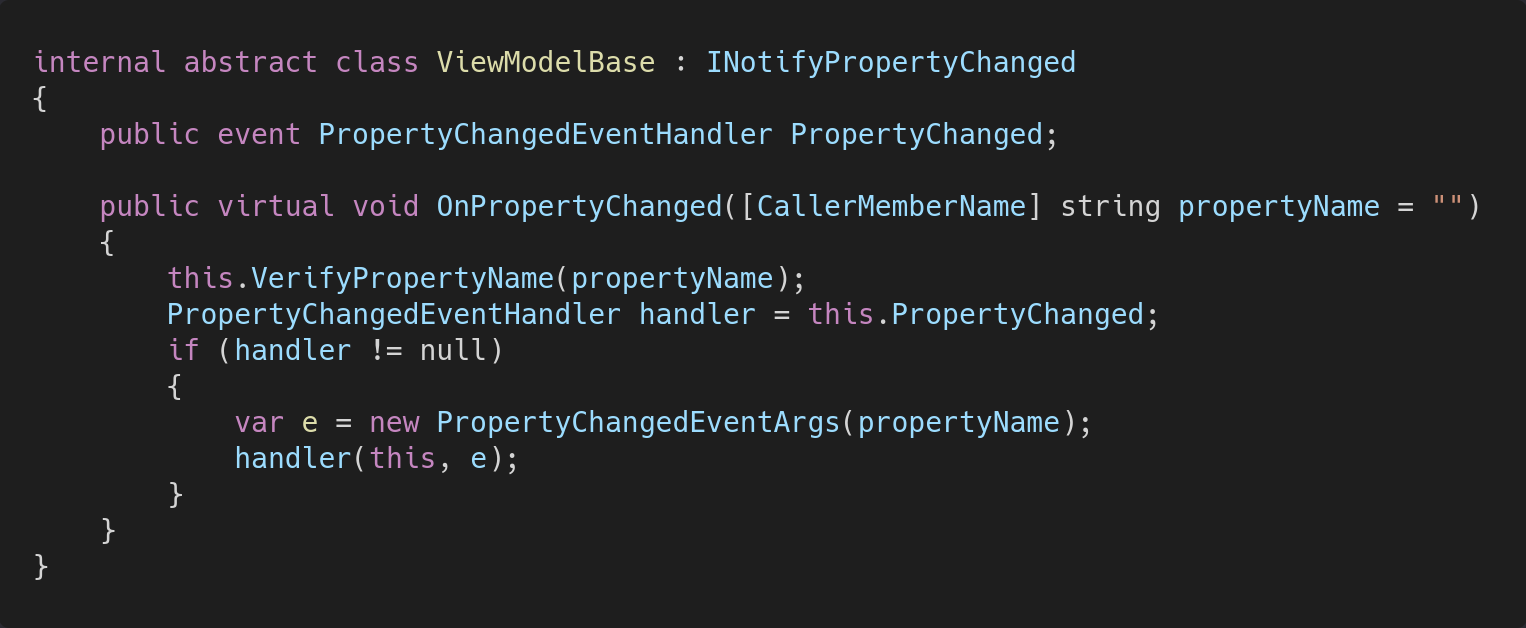
\includegraphics[width=\textwidth]{figures/code/mvvm-arch/viewmodelbase.png}
\caption{\texttt{ViewModelBase} implementation with \texttt{INotifyPropertyChanged} interface}
\label{fig:mvvm.viewmodelbase}
\end{subfigure}
\caption{Data binding notification implementation}
\label{fig:mvvm.databindingnotification}
\end{figure}

The notification raising and the implementation of the \texttt{INotifyPropertyChanged} interface can be seen in Figure \ref{fig:mvvm.databindingnotification}. The setter of \texttt{DiffusionInputKey} raises multiple notifications because other variables which depend on \texttt{DiffusionInputKey} also need updating. (The first call of \texttt{OnPropertyChanged}  in the setter has no argument because the attribute \texttt{CallerMemberName} in the function signature automatically enters the name of the caller if no argument is provided.)

On page exit, \texttt{ChaChaPresentationViewModel}, which is the view model which implements navigation between the different pages (which have their own view models), calls \texttt{Teardown} on the page we are leaving. This triggers the ChaCha execution with the given altered values.

Before execution, a flag was set which instructs the list getters into which the ChaCha component would save its intermediate values to return a different list. This means that the ChaCha component is agnostic of where it ultimately saves its intermediate values. During the execution, the intermediate values for the diffusion run are therefore saved in parallel lists. This is shown exemplary for the quarter-round input values in Figure \ref{fig:mvvm.chacha}. The other pages then simply bind to these lists to display the intermediate values of the diffusion run. Converting the 32-bit unsigned integers into hex strings and marking their characters which are different red is then done in the view models.

\begin{figure}
\centering
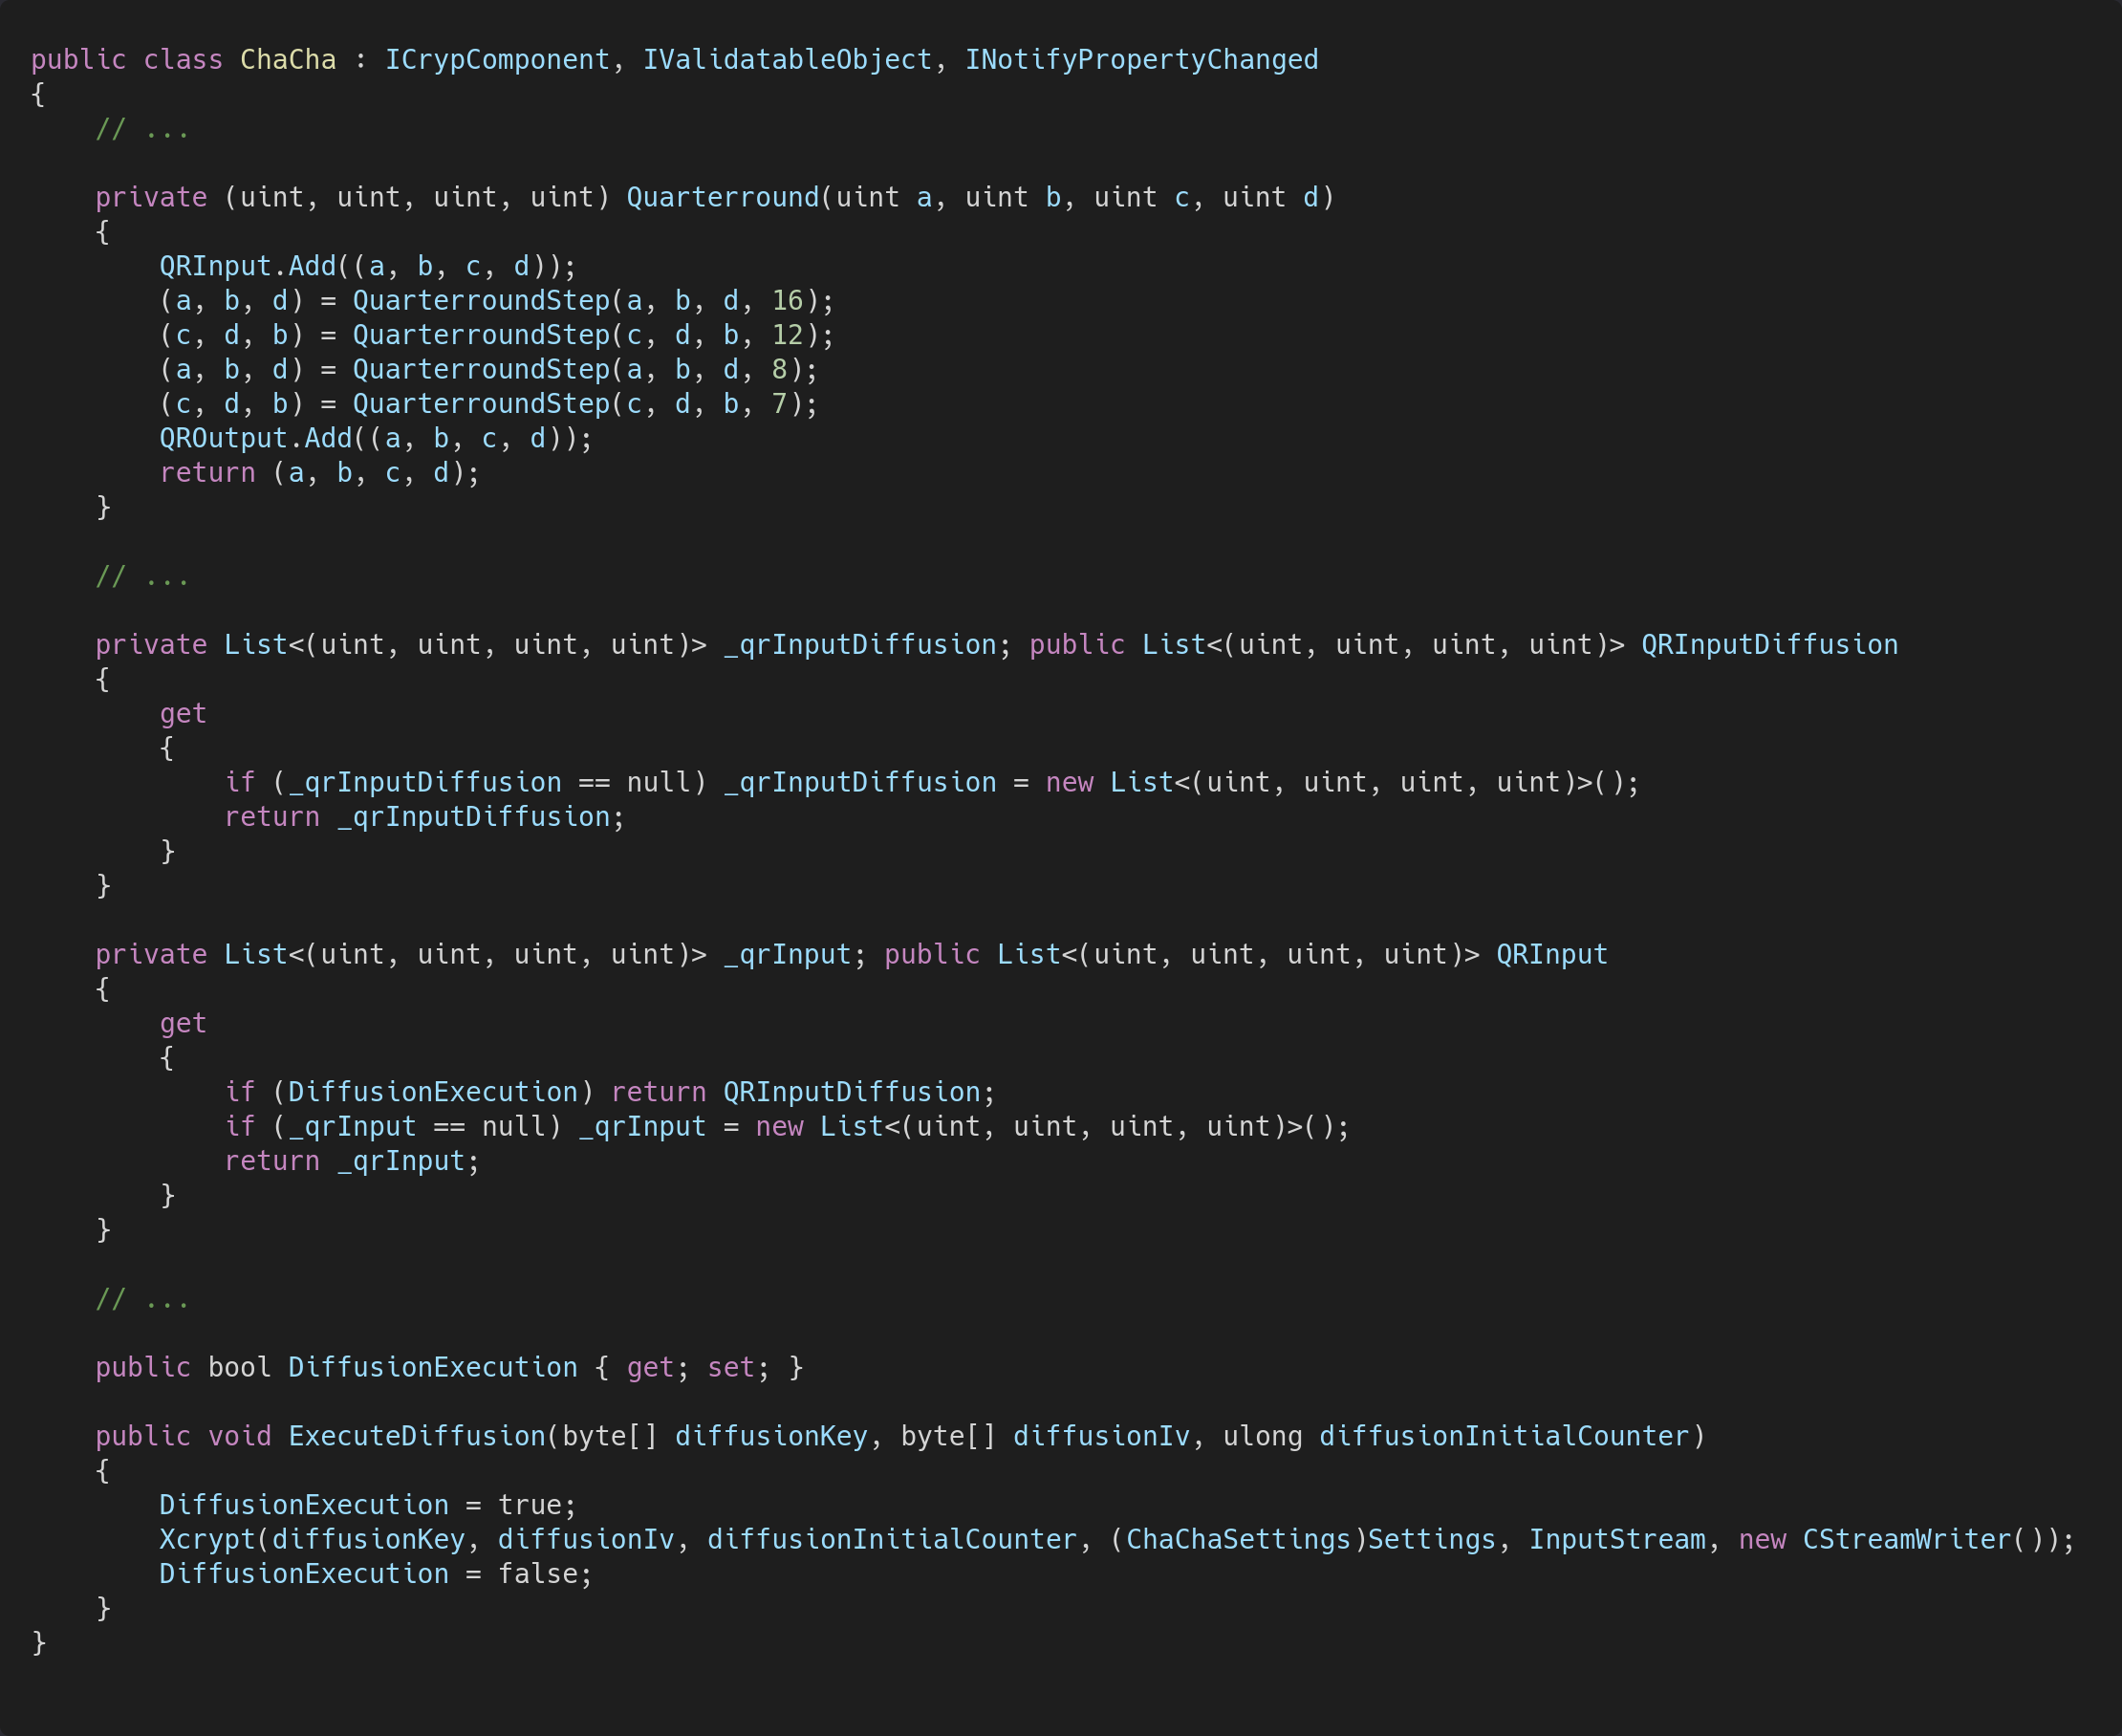
\includegraphics[width=\textwidth]{figures/code/mvvm-arch/chacha.png}
\caption[Intermediate values saving]{Saving of intermediate values during ChaCha execution in lists}
\label{fig:mvvm.chacha}
\end{figure}

\vfill

\FloatBarrier

\subsubsection{Centralized navigation system}

\begin{figure}
\centering
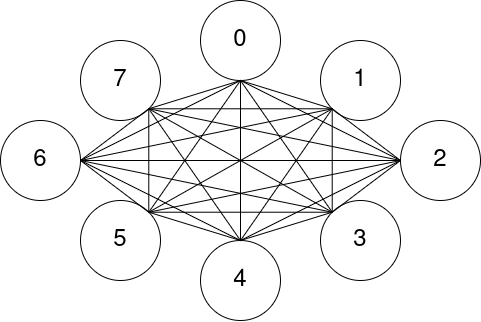
\includegraphics[width=0.5\textwidth]{figures/navigationsystem-diagram/navigationsystem-all-overview.png}
\caption[Navigation paths (no reset state)]{Navigation paths between actions if no reset state was used.}
\label{fig:navsystem.all.overview}
\end{figure}

The final design of the navigation system is characterized by reflecting on the problems previous iterations had. In this subsection, only the current, final implementation of the navigation system will be described. Previous implementations with their problems are described in Section \ref{sec:encounteredProblems}.

The core idea of the navigation system was to decrease hops between actions without having too many possible transitions since for every transition from action $A$ to another action $B$ and vice versa, code needs to be written to perform the transition. Figure \ref{fig:navsystem.all.overview} shows how a navigation system would look like where the maximum amount of hops is minimized to one. Total transitions are $2n(n-1)$ and for every new action, transitions increase by $2(n-1)$ ($n$ is the total number of actions). The factor 2 comes from the fact that for every transition from action $A$ to $B$, a transition back from $B$ to $A$ is also needed. We can conclude that such an architecture does not scale very well from the perspective of a developer who needs to write all of that transitional code. \\
On the other hand, decreasing the amount of possible transitions by introducing more hops would degrade performance due to computational overhead, so a system with a very high average amount of hops would not scale very well regarding performance.

\begin{figure}
\centering
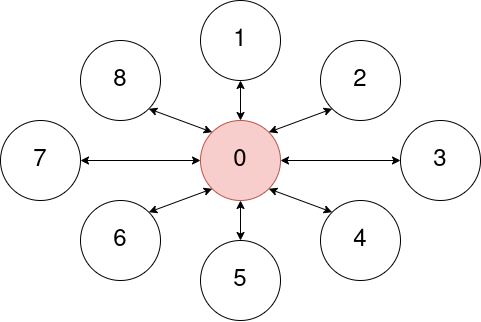
\includegraphics[width=0.5\textwidth]{figures/navigationsystem-diagram/navigationsystem-central-overview.png}
\caption[Navigation paths in centralized navigation system]{Navigation paths between actions in the centralized navigation system. \\The colored state is the reset state which corresponds to the initial state.}
\label{fig:navsystem.central.overview}
\end{figure}

We came to the conclusion that the best trade-off would be to have a navigation system where every action has a transition to a centralized state and this central state then has a transition to all other actions. This would result in a maximum of two hops between any two actions. Further, adding a new action would only add two new transitions to the system. This system design is shown in Figure \ref{fig:navsystem.central.overview}.

During implementation, it turned out that the amount of new transitions for each action could be decreased to one. Defining the initial state as the central state meant that transitioning from any action to it could be done by just resetting the whole page to the first action. Due to this, the central state can also be called the reset or initial state.

Unfortunately, the issue of code duplication quickly arised with this design. Since most of the time, the next page state was only a slight modification of the previous page state, the code for following actions was almost the same. To mitigate this issue, we started to think about the actions as \textit{sequences}. A sequence of actions would mean that every action inside a sequence is an extension of all previous actions of the same sequence. Extension in this context means that if action $A$ extends action $B$, action $A$ contains at least all the code of action $B$. To use terminology of set theory, one could also say that $A$ is a superset of $B$; viewing individual code statements as objects.

\begin{figure}
\centering
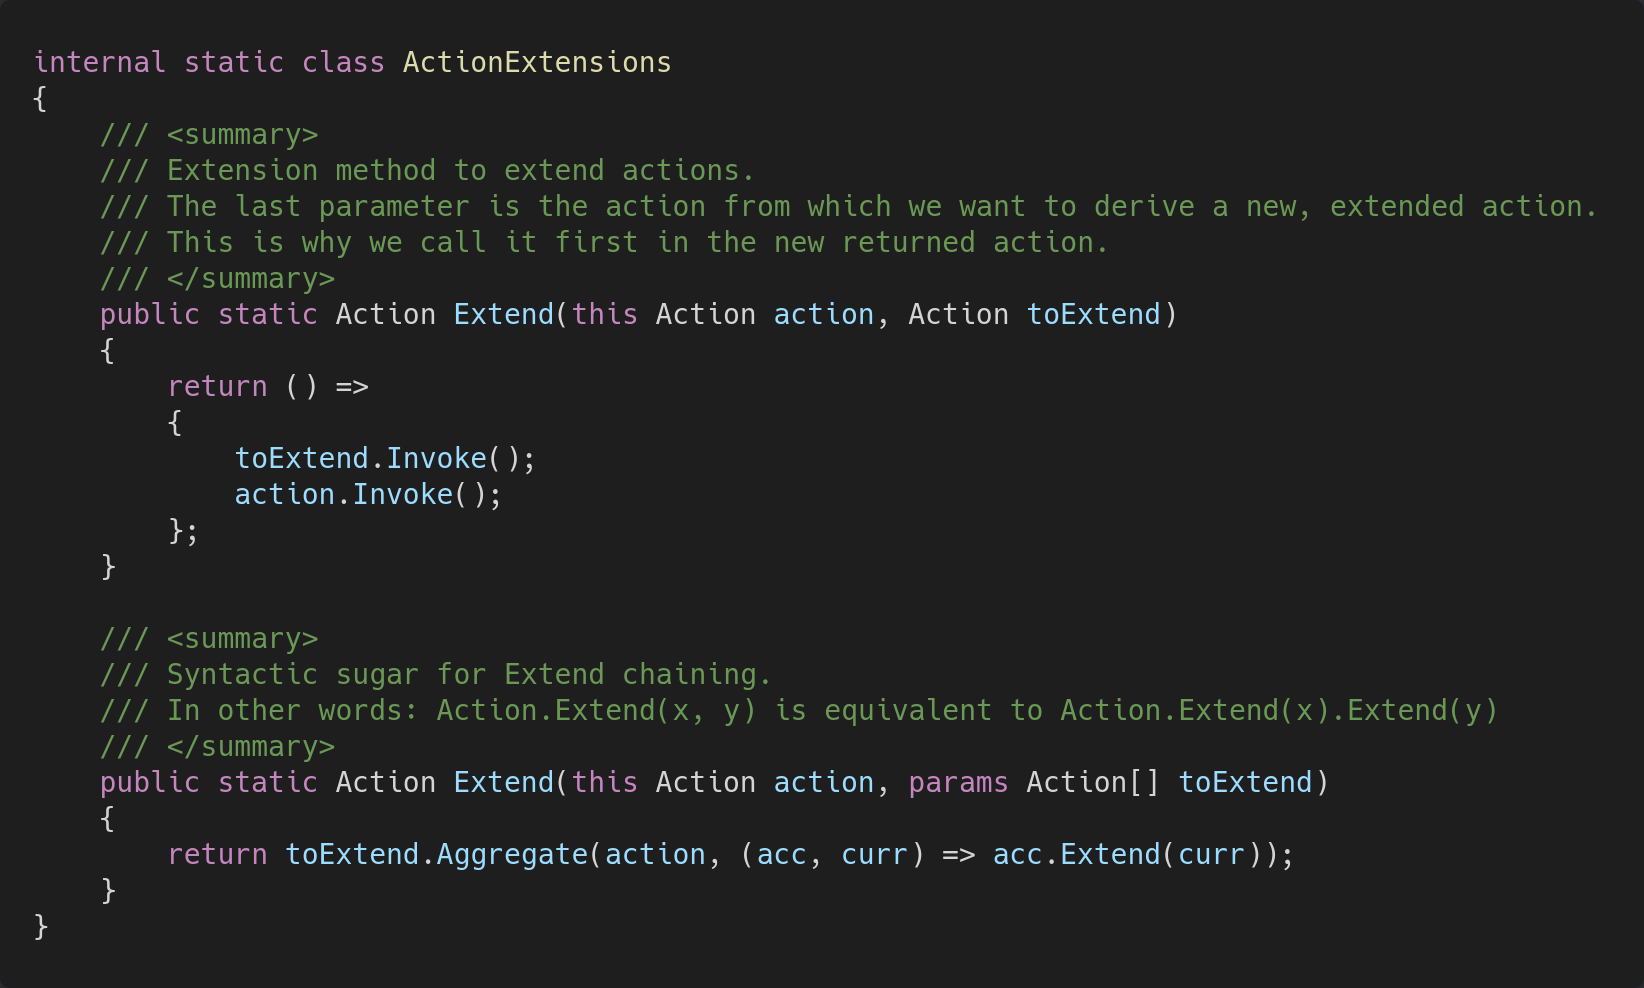
\includegraphics[width=\textwidth]{figures/code/nav-arch/action-extensions.png}
\caption[Extending \texttt{Action} type]{Extension method for the \texttt{Action} type to extend actions}
\label{fig:navsystem.sequences.extension}
\end{figure}

To implement this concept, an extension method for the \texttt{Action} type in C\# was created together with an interface to create action sequences. Figure \ref{fig:navsystem.sequences.extension} shows the method which extends the built-in \texttt{Action} type.

This concept was further developed by introducing \textit{nested sequences}. This means that a sequence could be started inside another sequence. A nested or child sequence would extend all the actions from its parent sequence. From the perspective of the nested sequence, it is no different than if all the actions from the parent sequence were created inside it. When ending a nested sequence, from the perspective of the parent sequence, the nested sequence never existed. Figure \ref{fig:navsystem.test} shows a test which asserts that this nesting does indeed work as expected.
\begin{figure}
\centering
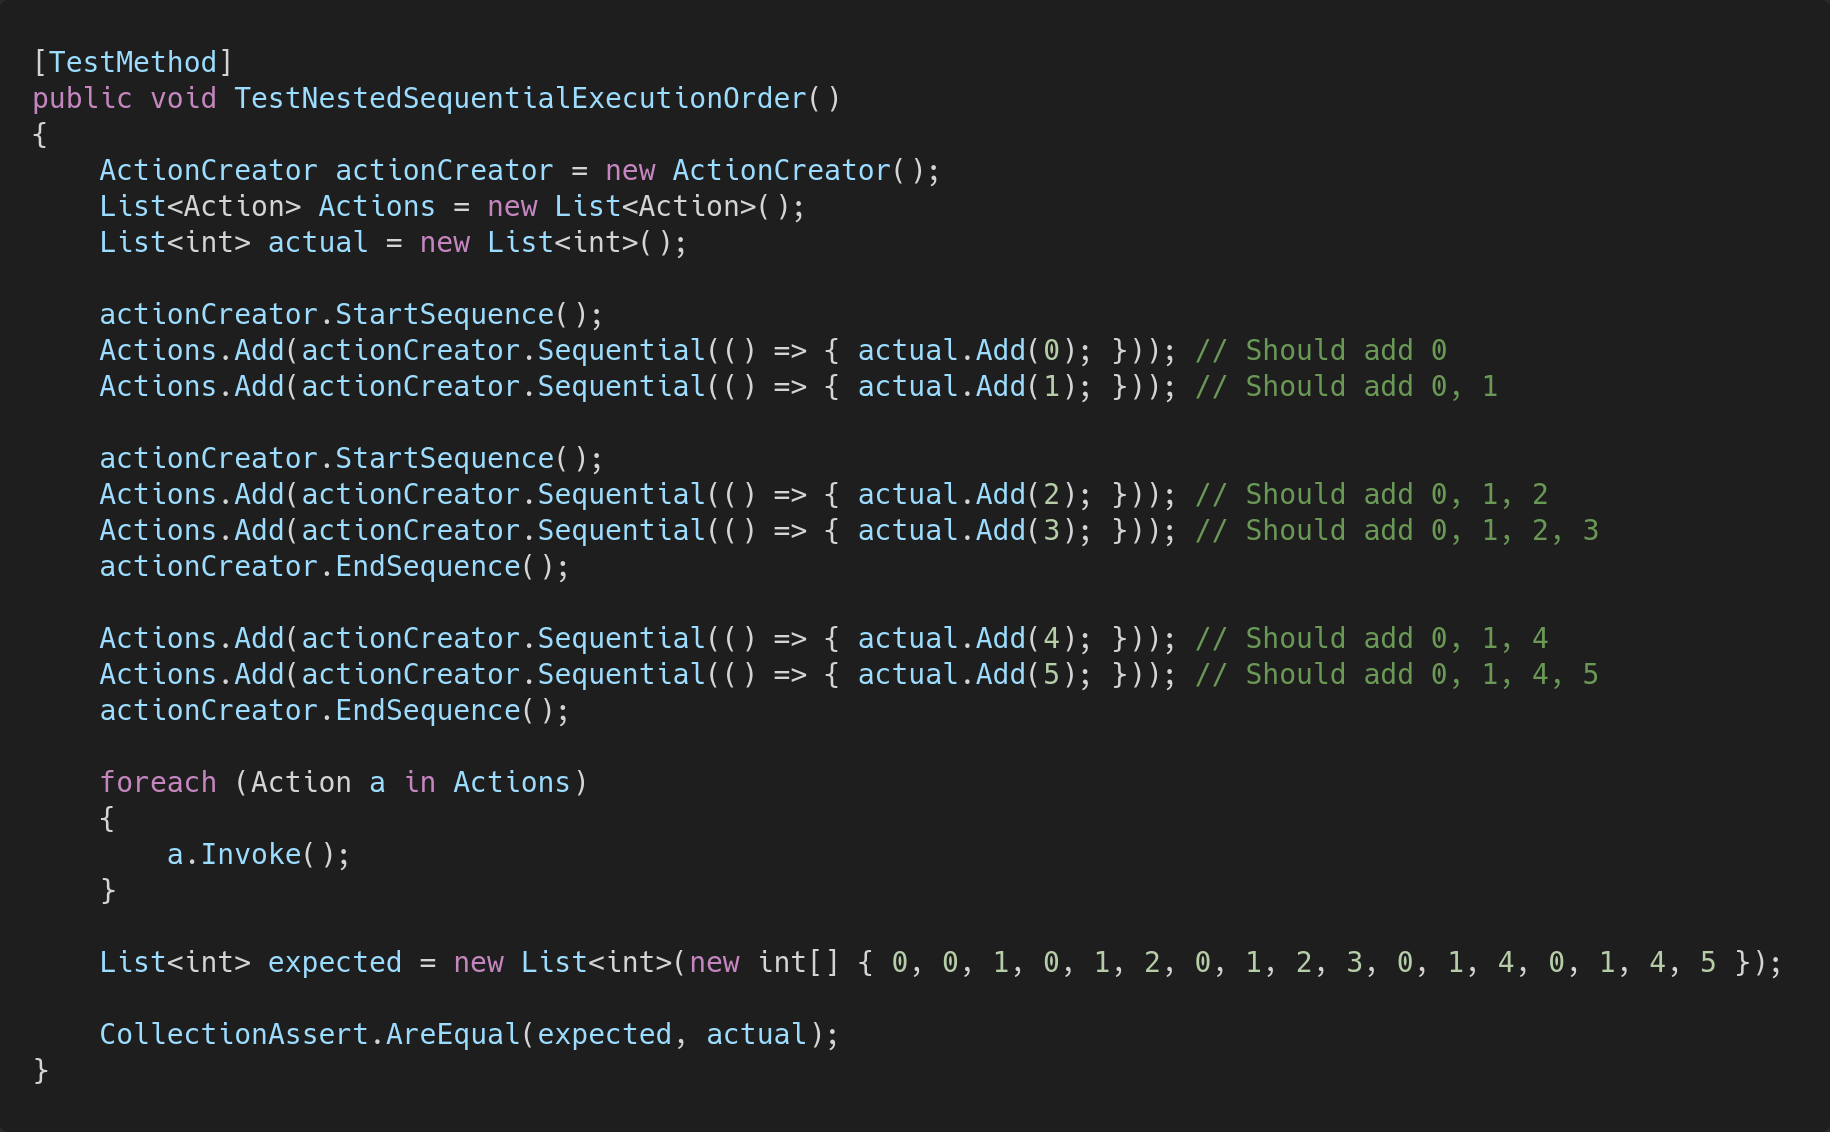
\includegraphics[width=\textwidth]{figures/code/nav-arch/TestNestedSequentialExecutionOrder.png}
\caption{Test method for nested sequences}
\label{fig:navsystem.test}
\end{figure}

Nesting sequences was very helpful for implementing the actions for the ChaCha Hash Function page. Since each keystream block started with a cleared quarter-round visualization and the initial state visible in the state matrix, it made sense to declare a sequence for each keystream block. Similar was true for the beginning of each round and quarter-round. Therefore, the sequences for the rounds were nested inside the keystream block sequence and the sequences for the quarter-rounds were nested inside the round sequences. This meant that I would not introduce too much computational overhead inside the transitional code (even though only one transition was executed by design) since I could just reset the sequence if it made no longer sense to include the code of previous actions. This was the case when a (quarter-)round or keystream block was finished.

Being able to nest sequences essentially prevented the system degrading back to a linear navigation system as will be described in Section \ref{sec:encounteredProblems}. The system would have less transitions but would still execute the same code as a linear navigation system would when moving from action 0 to any other action; undoing any positive effect this approach of minimizing transitions could have had.

The weakness of this design was that there was still some overhead when navigating through the page in a linear manner since the system is basically designed to always go back to the first action first and from there to the desired action. This leads to a lot of unnecessary resetting because as mentioned, most of the times the next page state is only a slight modification of the previous one. But this is the trade-off that was had to be made for a good overall performance. To summarize, this design had a higher overhead for small steps but did scale much better for bigger steps which were necessary for the keystream, round and quarter-round navigation.

The following section will make it clear why so much thought was put into the navigation system design. It will show why previous less thought-out architectures failed and includes plots about the performance of each architecture at the end.
%%%%%%%%%%%%%%%%%%%%%%%%%%%%%%%%%%%%%%%%%%%%%%%%%%%%%%%%%%%%%%%%%%%%%%%%

\section{Encountered Problems}
\label{sec:encounteredProblems}

This section will discuss the main problems that were encountered during implementation. To briefly summarize, they mainly consisted of how the system behind the interface should be designed to have the best or at least a reasonable performance.

As described in Chapter \ref{sec:aesVisualization}, to enable a fluent navigation experience where the user can navigate very freely through the visualization (using backward and forward navigation), the intermediate values need to be pre-calculated. But as will be explained on the next pages, this was not all that was needed to ensure such an experience.

We hope that the description of these problems and the solutions we have found may help future students in writing their own plug-ins.

\subsubsection{Linear navigation system}

\begin{figure}
\centering
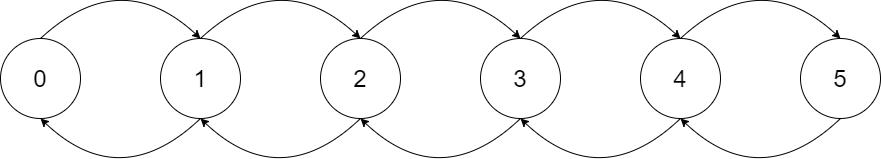
\includegraphics[width=\textwidth]{figures/navigationsystem-diagram/navigationsystem-linear-overview.png}
\caption[Navigation paths in linear navigation system]{Navigation paths between actions in the linear navigation system}
\label{fig:navsystem.linear.overview}
\end{figure}

The performance of the plug-in was essentially coupled to how the navigation system was designed. Other things like the aforementioned calculation of the intermediate values for the visualization were compared to the navigation system design insignificant because they are created by the ChaCha cipher anyway and must just be saved somewhere to not lose them. This means that storing them was only a necessary but not sufficient condition for a overall good performance.

This was noticeable for the first time early during the implementation of the action input field. This input field would enable the user to skip from any action to any other action. During testing, the performance of the navigation system turned out to be a problem. Skipping 100 actions took about 750ms during which the UI was unresponsive and this would only get worse the more actions were skipped. As can be seen in Figure \ref{fig:navsystem.performance.linear}, this time increased linearly so it was quite clear that something needed to be done about this, especially because the page with the most actions had over 3000 actions. All measurements were taken by starting at action 0 and skipping to the action specified at the x axis.

The root cause of the problem was the navigation system design which was called in hindsight \textbf{\textit{linear navigation system}}. It consisted of defining actions which build upon each other. This means that if we are at action 0 (initial state of the page) and want to go to action 5, we need to execute all the code inside the action definitions between 0 and 5 to arrive at the page state as it should be at action 5. This is resembled in Figure \ref{fig:navsystem.linear.overview}.

This linear navigation system design was used to have a smooth implementation experience since one has to only write the actual page state changes between to actions. Code duplication was prevented because pages most of the time only changed a little bit between steps and thus the page state of each action is best described using differences. This complemented how the user experiences the visualization. The actions are numbered in a sequence and thus are inherently linear. Because of this, reflecting this linear nature in the system design made a lot of sense.

Since this "design flaw" was not the leading cause of the performance problem (going through a for-loop of size 3000 does not directly lead to performance issues), we will continue with briefly explaining how the actual code responsible for the transitions looked like.\\
During the transition between two page states, the state of the page elements which will change is saved such that we can undo the changes if the user decides to navigate back. This enabled ``automatic action undoing'' and thus to skip writing transitional code for backwards navigation. A function was written which retrieved the state corresponding to the transition and then applied it. This function worked for all backwards navigation without further intervention which was very convenient during development. \\
The problem with that architecture was that the state saving and the execution logic inside the action definitions were changing a lot of page elements directly by accessing them via their name that was given to them in the XAML code. This issue combined with the restricted, linear pathing between actions resulted in that significant performance loss that was described in Figure \ref{fig:navsystem.performance.linear}.

\subsubsection{Linear navigation system with caches}

After identifying the two underlying issues, a \textbf{\textit{linear navigation system with caches}} was implemented. As the name suggests, cache entries were implemented to be able to navigate in constant time between an action and an action which was cached. To not only increase performance during these transitions (action to cached actions) but between all transitions, we check before each transition, if first moving to a cached entry would decrease the amount of hops needed to go to our destination. If this is true, we first go to the cached entry and then to our destination. Figure \ref{fig:navsystem.cache.overview} demonstrates that such a  navigation system needs less hops between any two given actions.

\begin{figure}
\centering
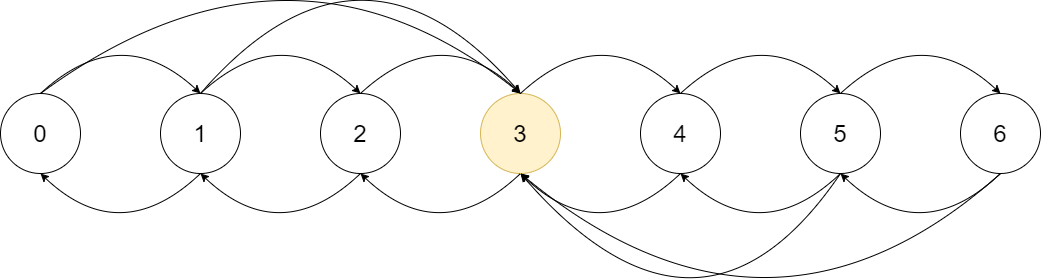
\includegraphics[width=\textwidth]{figures/navigationsystem-diagram/navigationsystem-cache-overview-2.png}
\caption[Navigation paths in linear navigation system with caches]{Navigation paths between actions in the linear navigation system with caches. The colored state has a corresponding cache entry.}
\label{fig:navsystem.cache.overview}
\end{figure}

The cache entries consisted of instructions to restore the complete state of a page at the action index for which this cache entry was for. They contained instructions for the complete state instead of only the difference between two actions because now, moving to that cache must initialize the page, independent at which action / page state we were before. This means that there was some overhead in initializing the page because essentially, the whole page was cleared and then the the page elements with their appropriate content were initialized, potentially leading to some unnecessary code execution because the content prior to cleaning was already the one we needed. 

Nonetheless, creating a cache entry for every start of a round increased performance significantly as can be seen in Figure \ref{fig:navsystem.performance.qr}. The maximum response time went down from more than 40 seconds in the system without any caches to 1.5 seconds (!). This could further be decreased to 200 milliseconds by creating cache entries for every start of a quarter-round (see Figure \ref{fig:navsystem.performance.qr}). Since it was not feasible to time every single data point, the data points marked as squares were just interpolated using previously timed data points. This means that for example, for the interpolated cache data points, the average of all previous measurements for skips to cached actions was taken.

Further, to decrease the load on the CPU while dragging the action slider, a very simple asynchronous navigation was implemented. It was implemented by using a stack as a buffer for the values received from the slider during dragging. Every 50ms, the last value from the buffer is read and the page moves to that action. Afterwards, the buffer is cleared. \\
This did only enhance the slider but not the performance because at its core, it used the same navigation logic; just asynchronously. Nonetheless, it improved the user experience during dragging significantly which I found quite impressing for how minimal the code for it is. In fact, the whole code for the asynchronous navigation can be seen in Figure \ref{fig:async.navigation}. Before, dragging the slider lead to weird artifacts where the slider would jump forwards and backwards because the navigation was executed while dragging. Therefore, dragging the slider conflicted with the navigation system going to a certain action which would reset the slider to a certain position. Executing the navigation after dragging was finished was not an option because that basically made the slider useless.

One of the major drawbacks for this enhanced design  with caches was that the automatic action undoing was no longer possible. Since we can not guarantee that the state between two actions has been saved, we cannot use our undo function. Therefore, the code for backwards navigation needed to be written manually.

\begin{figure}
\centering
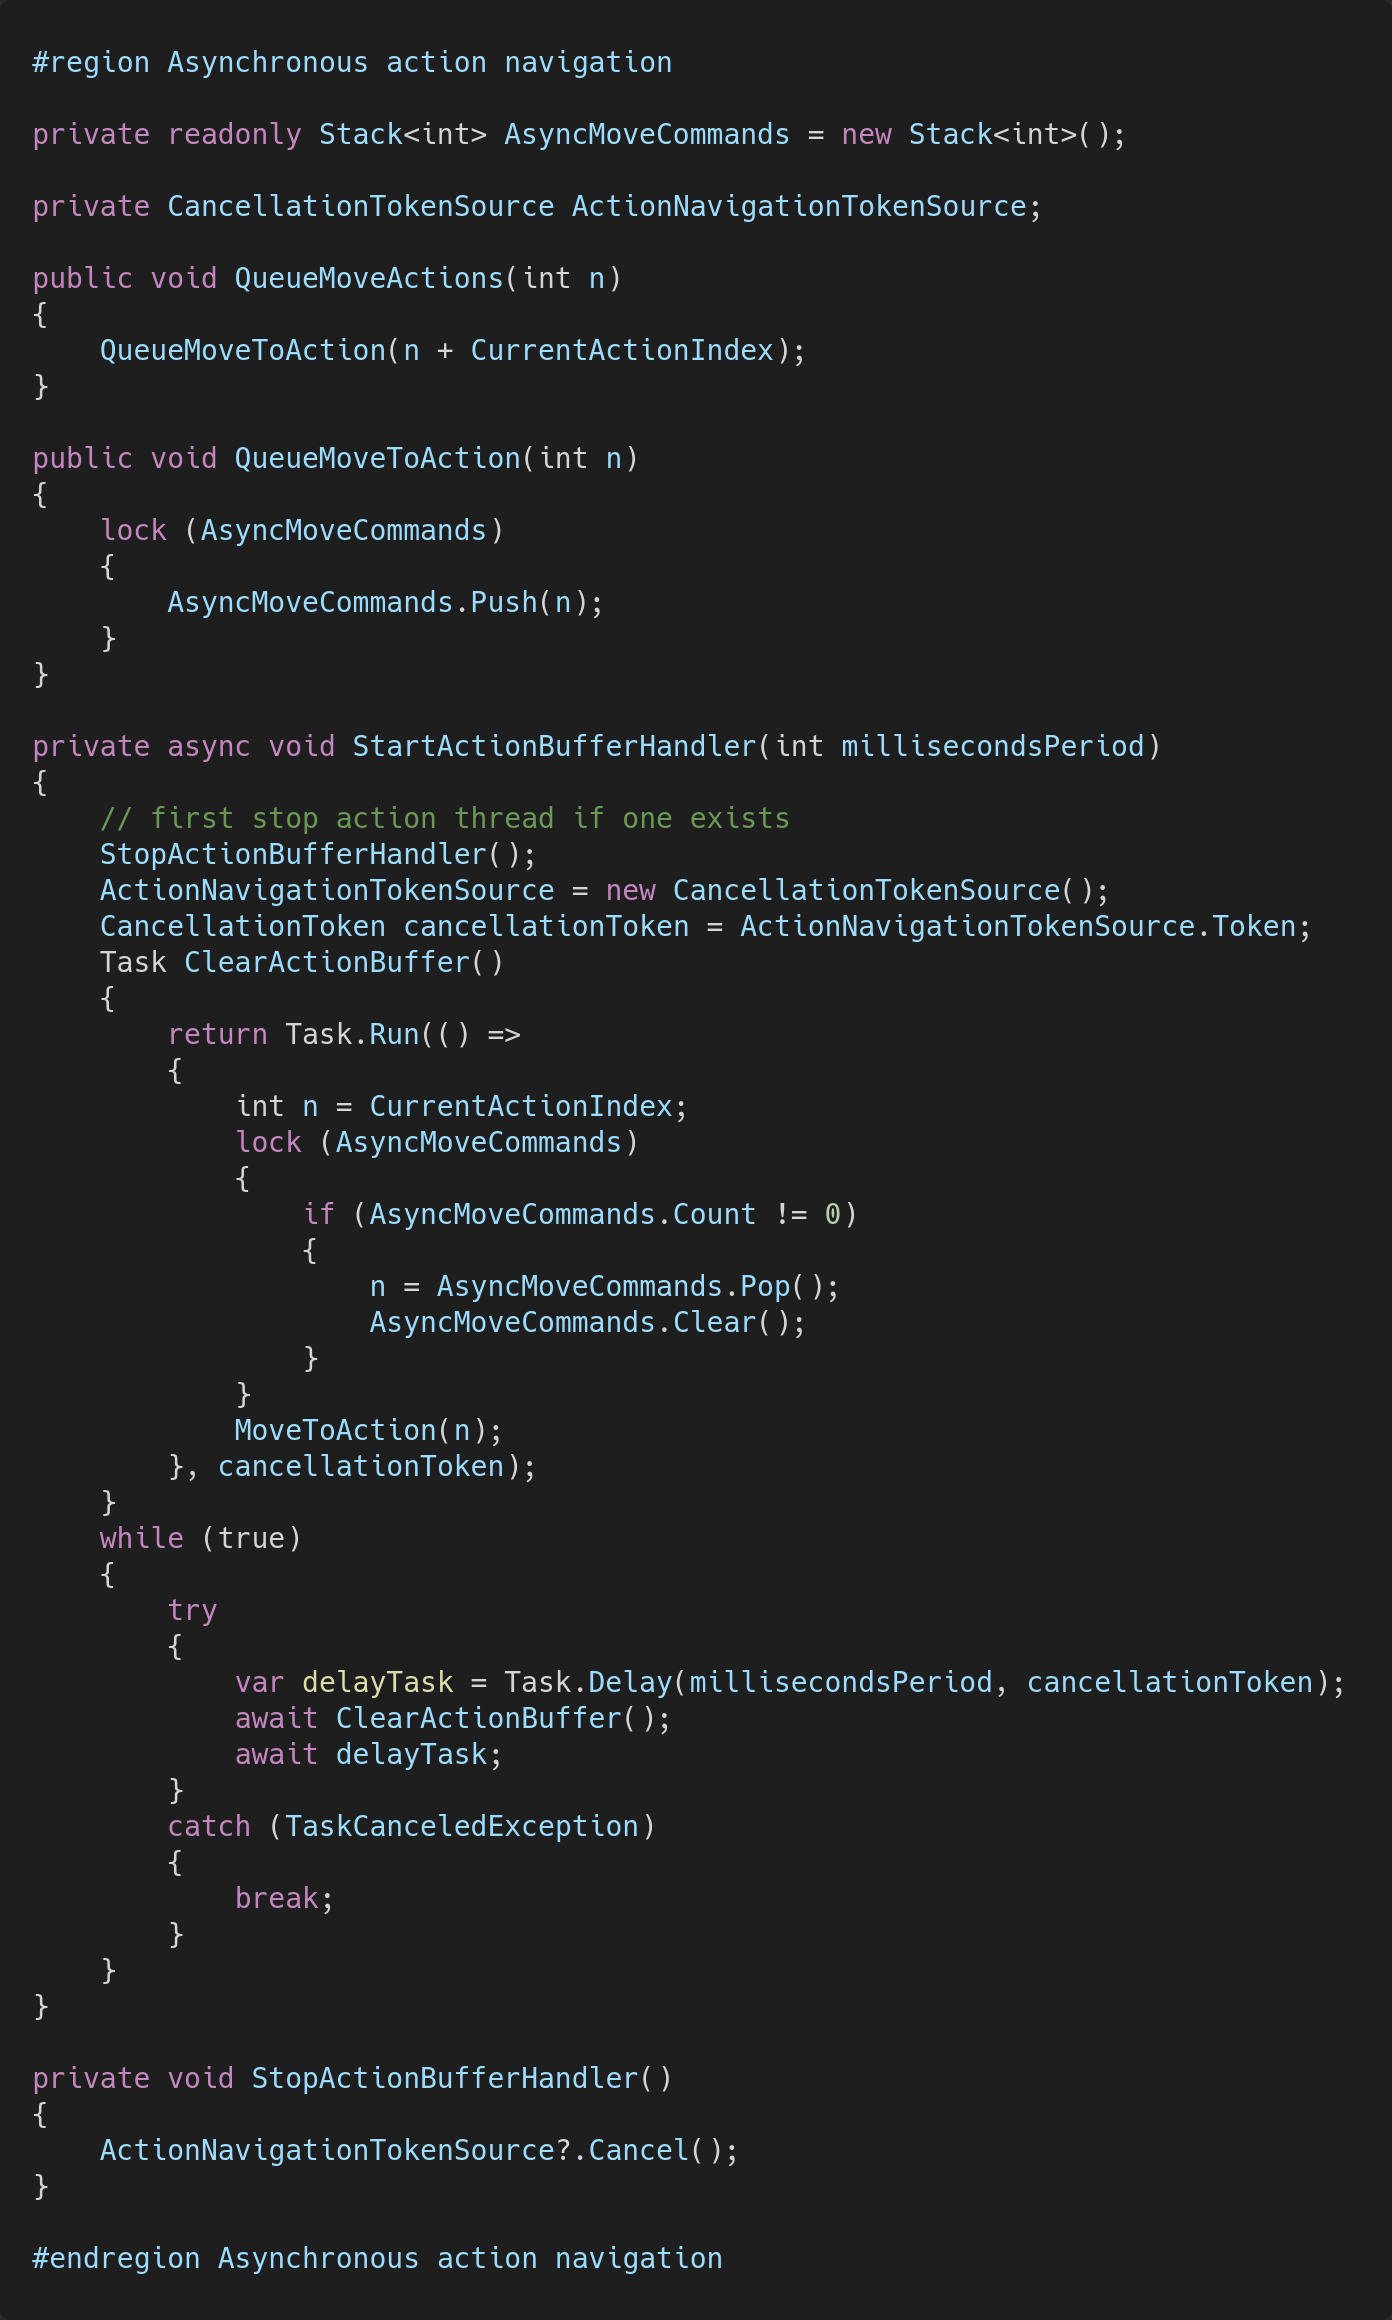
\includegraphics[width=0.85\textwidth]{figures/code/nav-arch/async-navigation.png}
\caption{Asynchronous navigation subsystem}
\label{fig:async.navigation}
\end{figure}

\FloatBarrier

\subsubsection{Centralized navigation system}

During the implementation of other features such as the diffusion, it was noticed that having to implement for each page action the forward and backwards code, the code became quite error-prone. It was hard to notice bugs because it was not feasible to check every single action from both directions manually and creating a testing framework just because of this was out of scope. \\
Some navigation bugs were easy to notice because due to the overall still linear nature of the navigation system, errors did propagate. This means that a error in a previous action most likely did break the page state on future actions because they depend on each other. \\
Nonetheless, this did not help in tracking down the bug because it was not known on which action the error happened. This only gave more reason to reiterate on the navigation system again.

To decide if the code only needs to be refactored or indeed rewritten from scratch, all current problems with the existing codebase were summarized. They not only consisted of performance problems but also with visualization problems. For example, resizing the window did not appropriately scale the UI elements as can be seen in Figure \ref{fig:plugin.scaling.bug}. Additionally, the current navigation system was quite restricted in what kind of UI elements it supported without further hassle. Since during the last navigation system update, the existing code was only updated, the core design was still all about directly manipulating and creating UI elements on demand. The existing functions revolved around the UI elements currently in use thus they could not easily be reused for different, new UI elements; leading to the mentioned limited support of the navigation system.

\begin{figure}
\begin{subfigure}{\textwidth}
\centering
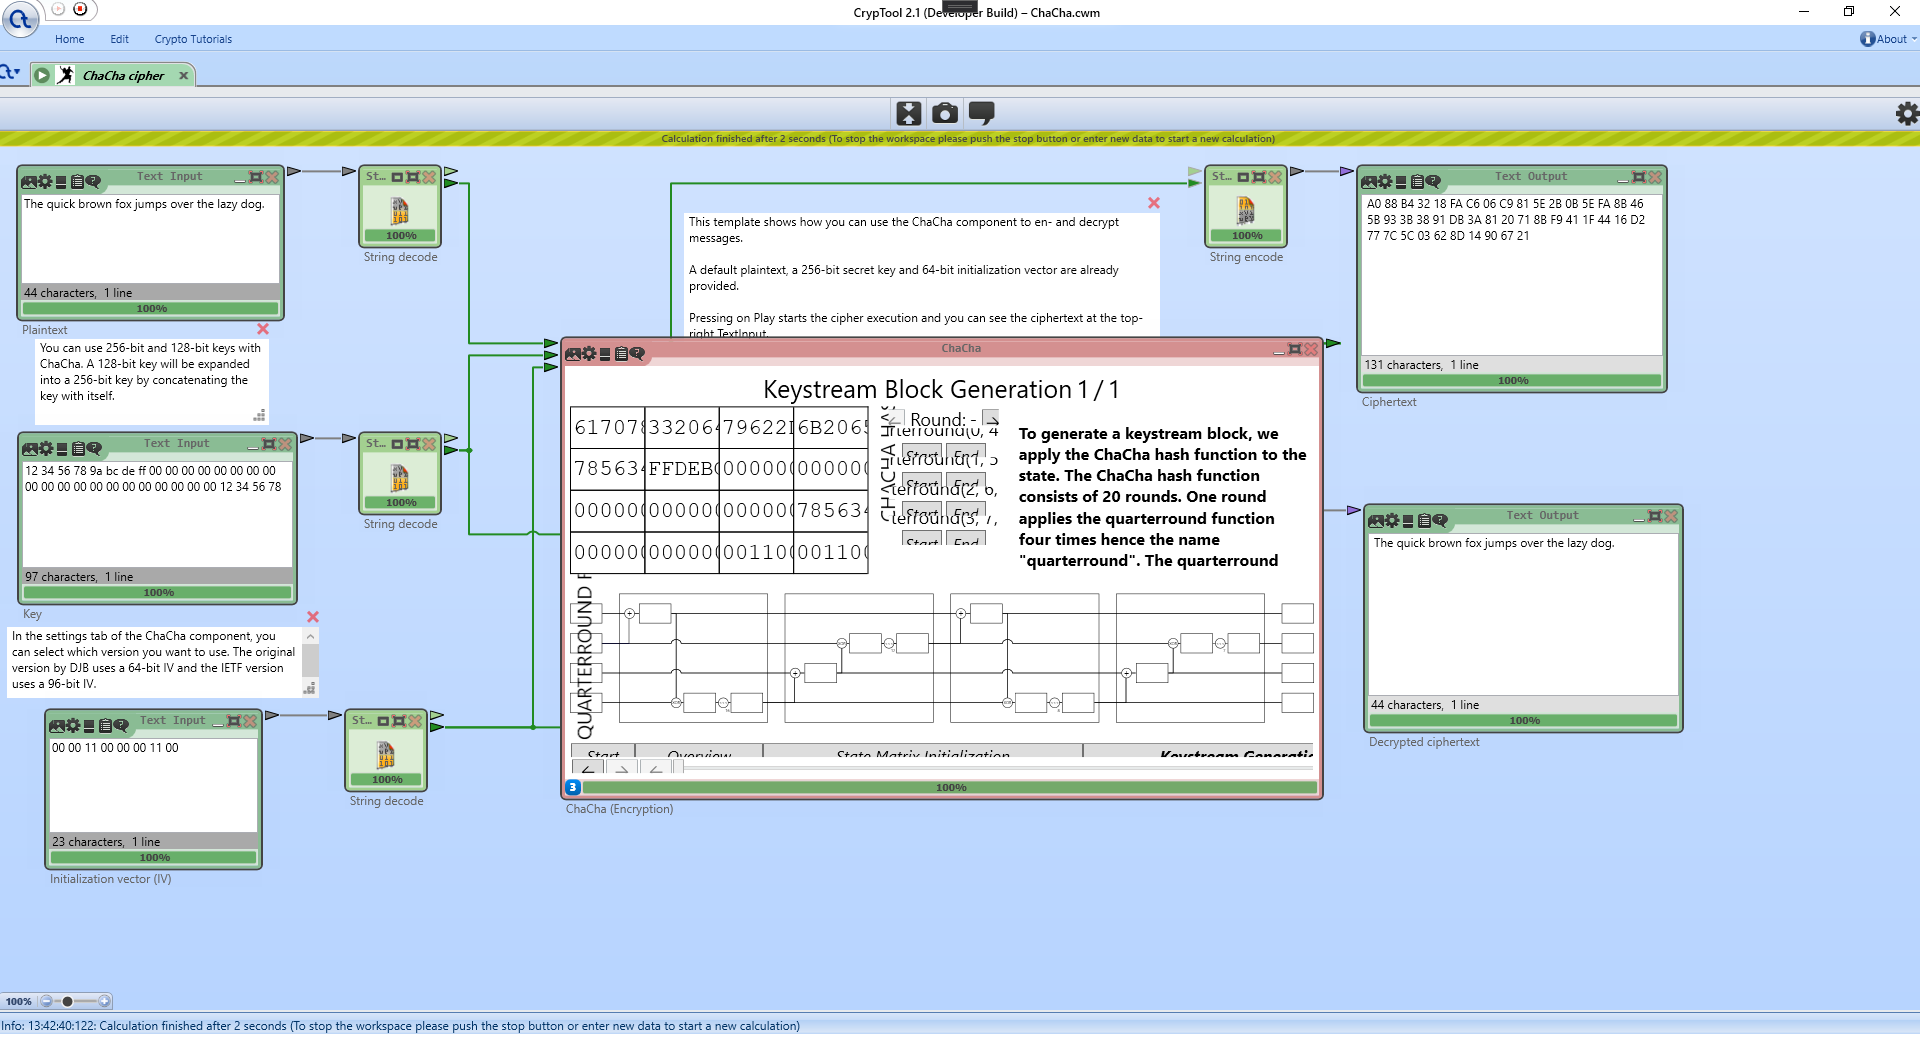
\includegraphics[width=\textwidth]{figures/ct2/scaling-bug-example.png}
\caption{Bad scaling property}
\label{fig:plugin.scaling.bug}
\end{subfigure}
\begin{subfigure}{\textwidth}
\centering
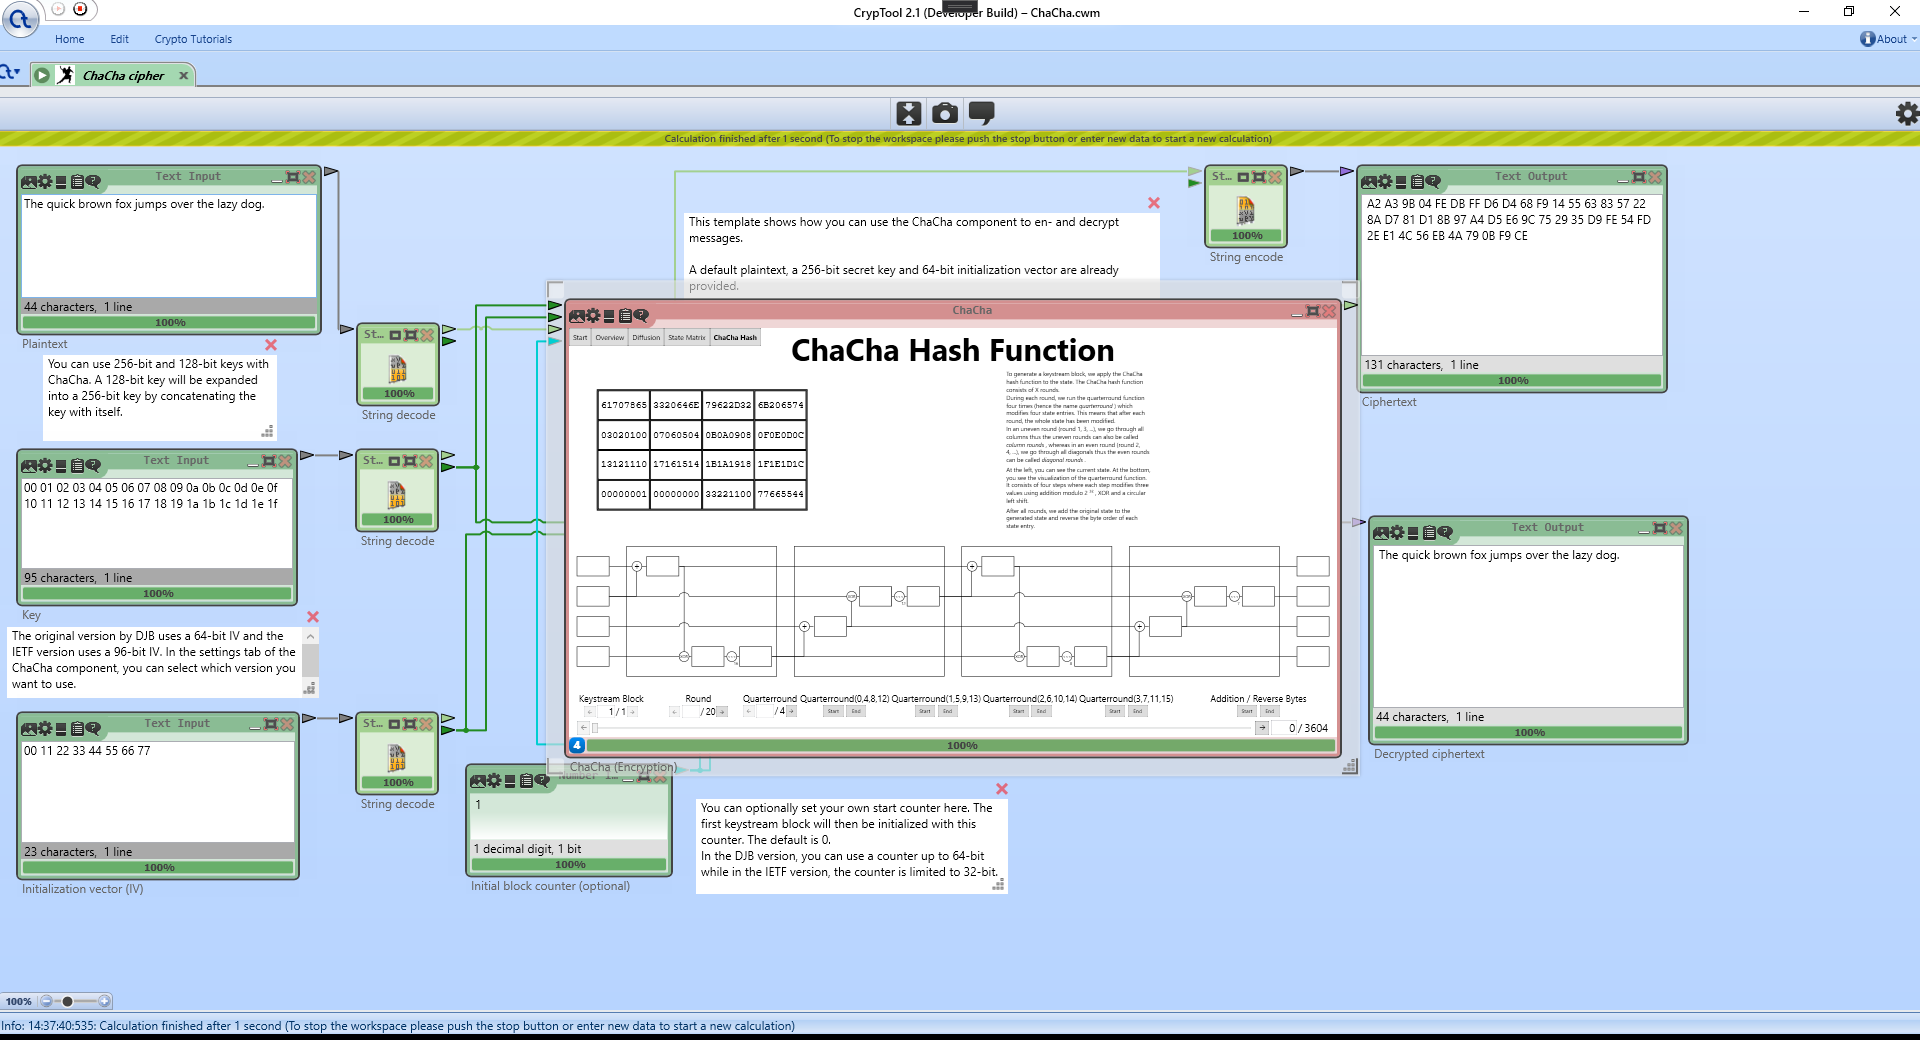
\includegraphics[width=\textwidth]{figures/ct2/scaling-bug-fixed.png}
\caption{Fixed scaling property}
\label{fig:plugin.scaling.fix}
\end{subfigure}
\caption{Example for bad scaling property in previous plug-in versions}
\end{figure}

Essentially, the problem was that a lot of the code-behind was highly coupled to the XAML code. This was done likt this because it was very straight-forward to do so and lead to fast results. At first, the trade-off between loss of maintainability/flexibility in the future and not having to spend precious time to learn design patterns for WPF applications seemed worth it. This thinking was grounded in the reason that the code for this bachelor's thesis would not get regular updates long into the future thus high maintainability or being easy to extend was not a priority. This assumption turned out to be false when realizing that the amount of "code smells" that could be handled was already to high about one month before the date of handing in the thesis. Every code change kept increasing the accumulated technical debt; killing any motivation still left to work on the existing code base. Continuing like this for another month seemed impossible. Therefore, a list of all current problems was created together with what requirements a new software architecture would need to meet to solve them:

\begin{description}
\item [(Inconsistent) Performance] The underlying linear design was crippling the performance for the reasons already mentioned. The introduction of caches did only fight the symptoms and not solve the main issue. Further, it made the performance confusing for the users. Sometimes, it took close to no time at all to move to a certain action (action was cached) and on other times, it took quite a lot of time to move to a different action (action was not cached). \\
\textit{\textbf{Requirement}}: Moving to any action should be done in $O(1)$. This means, it should not matter how many actions we needed to skip to arrive at the destination.
\item [Error-prone design for action creation] Writing new actions was error-prone because code needed to be written for forward and backwards navigation which introduced mental overhead because it depended on the code of all previous actions. This also lead to error propagation. Errors were easily noticeable by users but were hard to track down to their origin.\\
\textit{\textbf{Requirement}}: New actions should be able to be written without having to write backwards navigation code. Backwards navigation should be handled automatically and thus be "error-free by design".
\item [No coherent system design] Adding new code without following a design pattern made it hard to grasp the system architecture over the long run. Additionally, the high coupling of the backend (code-behind) with the frontend (XAML) made it harder to implement new features in one part without needing to modify the other part. The system essentially got very rigid and over time, even seemingly small changes took quite some time to implement.\\
\textit{\textbf{Requirement}}: The new system should make it clear what piece of code is responsible for what and thus be highly modular. This should also make it clear where new code must be added to implement a new feature without increasing technical debt; while also decreasing the possibility to introduce bugs since code is less coupled. To summarize, the new architecture should strive for high cohesion, but low coupling.
\end{description}

\begin{figure}[!hbt]
\centering
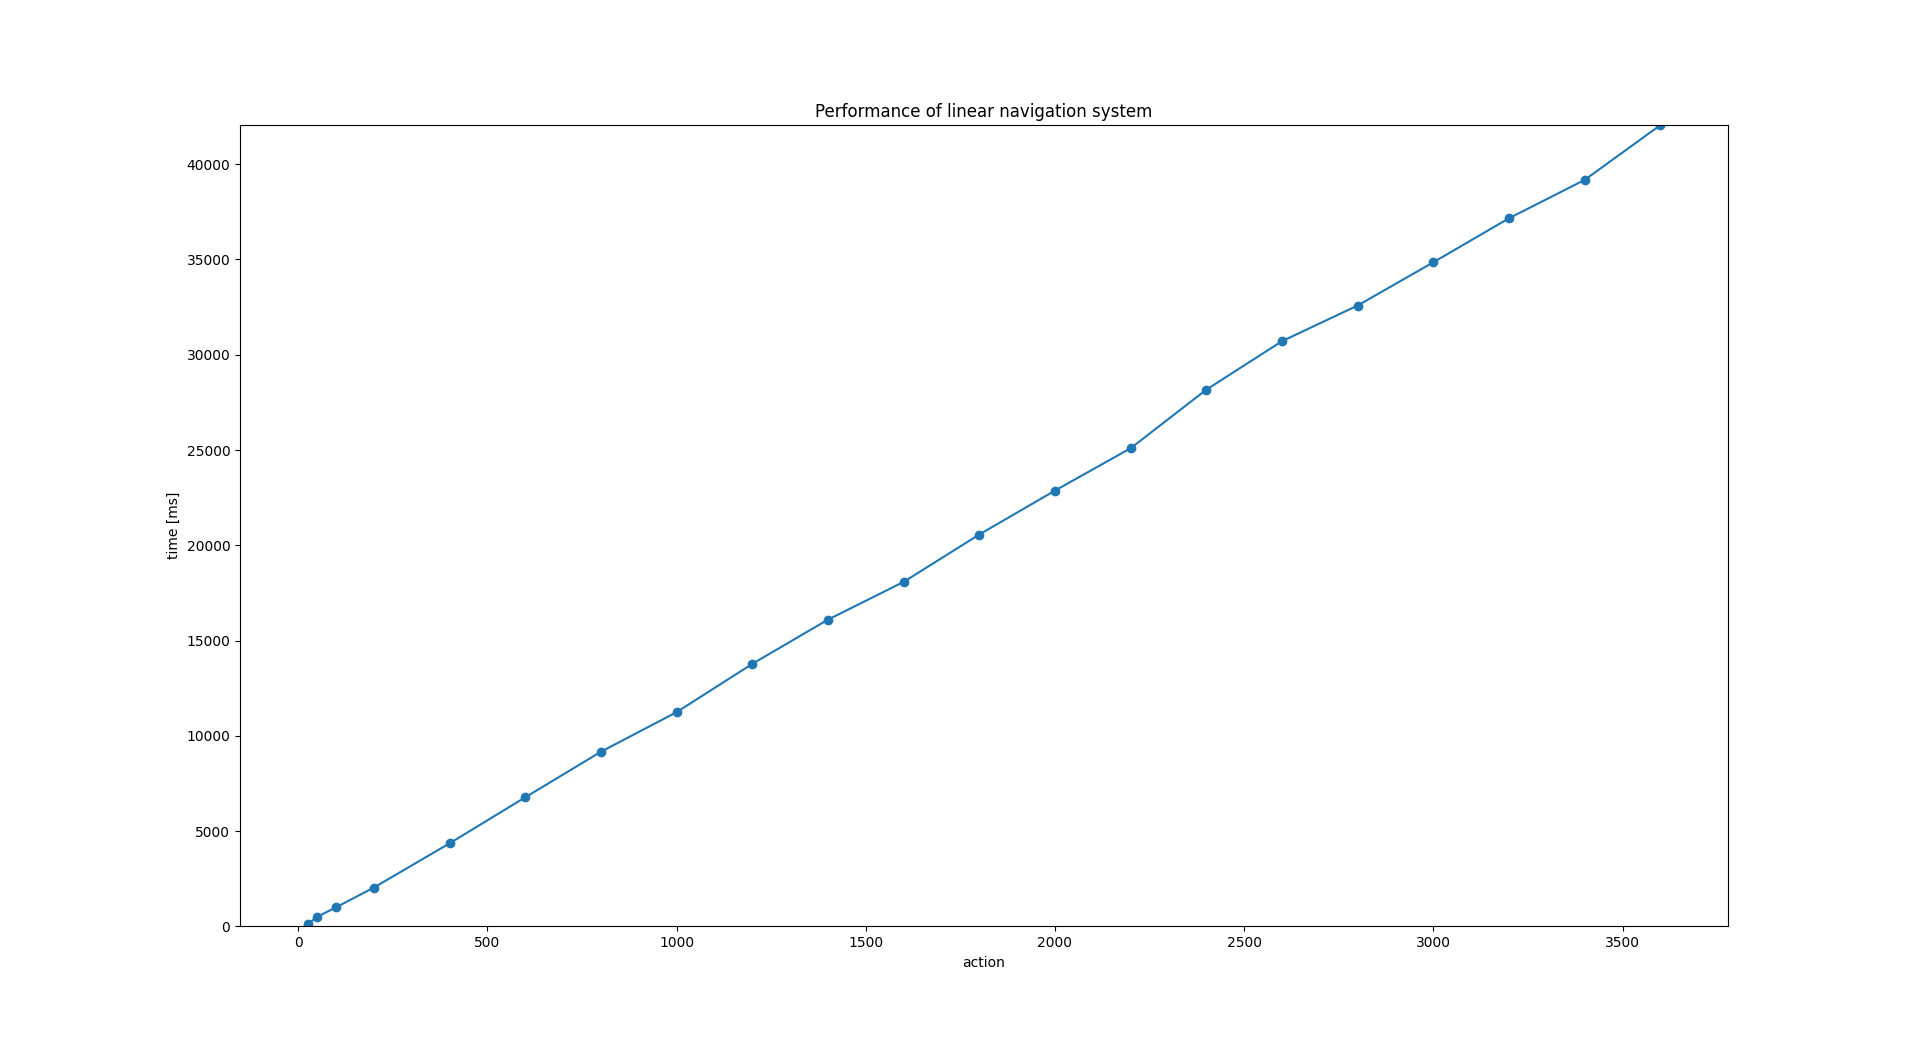
\includegraphics[width=\textwidth]{figures/pyplot/performance_navsystem-linear.png}
\caption{Performance of linear navigation system}
\label{fig:navsystem.performance.linear}
\centering
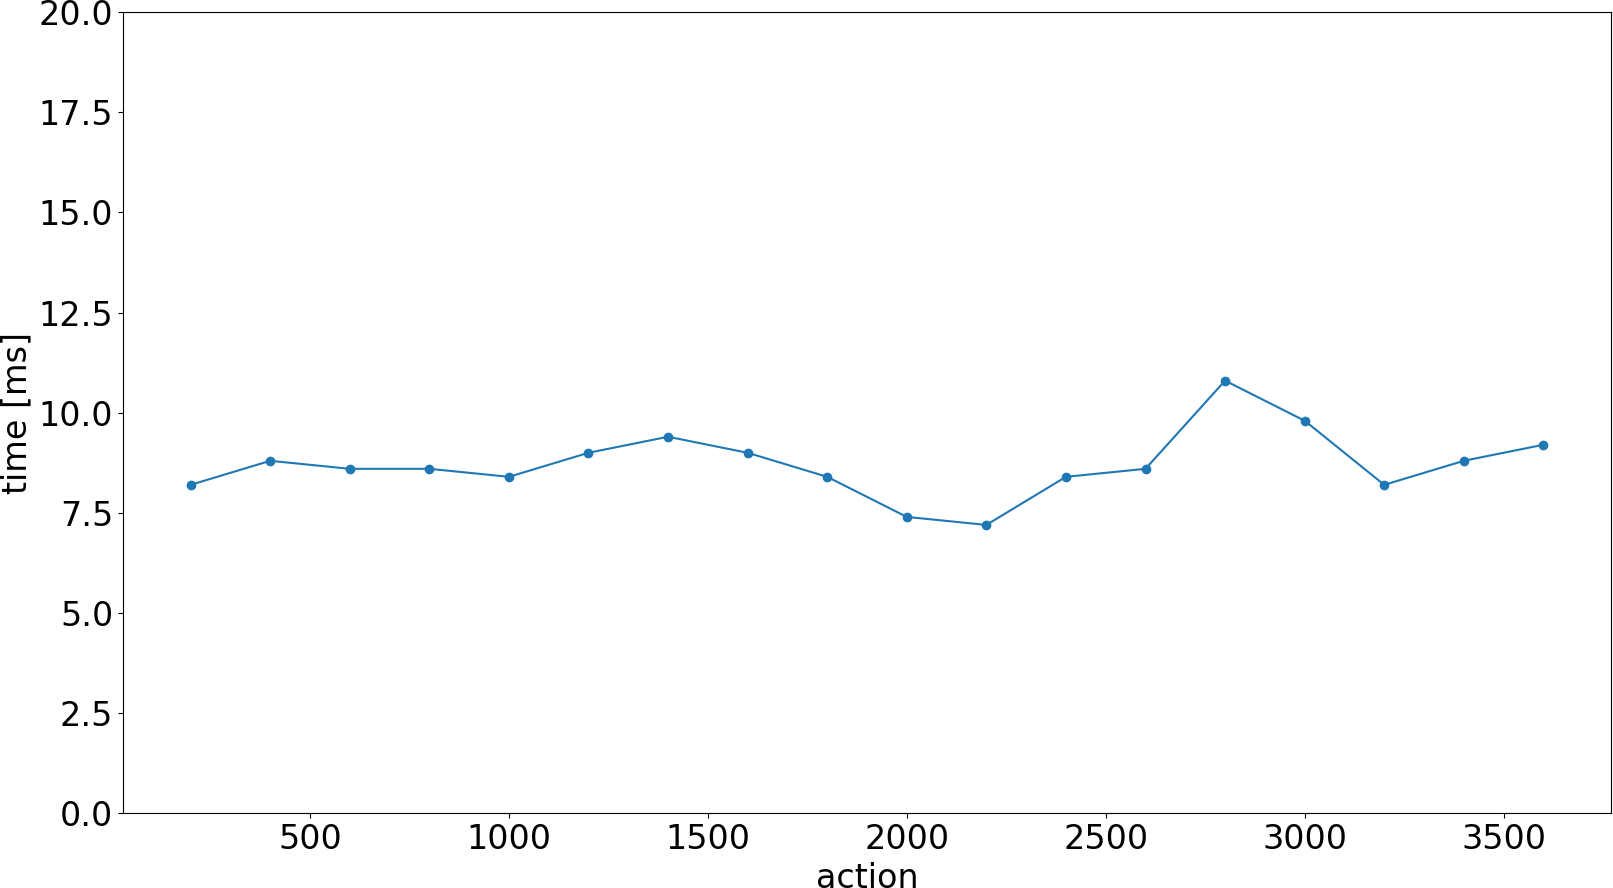
\includegraphics[width=\textwidth]{figures/pyplot/performance_navsystem-central.png}
\caption{Performance of final (centralized) navigation system}
\label{fig:navsystem.performance.central}
\end{figure}

\noindent
All these problems were solved using the MVVM design pattern with a new navigation system design. To implement them, the existing codebase was rewritten from scratch, which was time-consuming (took about two weeks) but in the end worth it. Figure \ref{fig:navsystem.performance.central} shows the performance of the final navigation system. As one can see, the time it takes to skip actions is constantly very low and only varies between a few milliseconds; making the user interface very responsive.

\begin{figure}
\centering
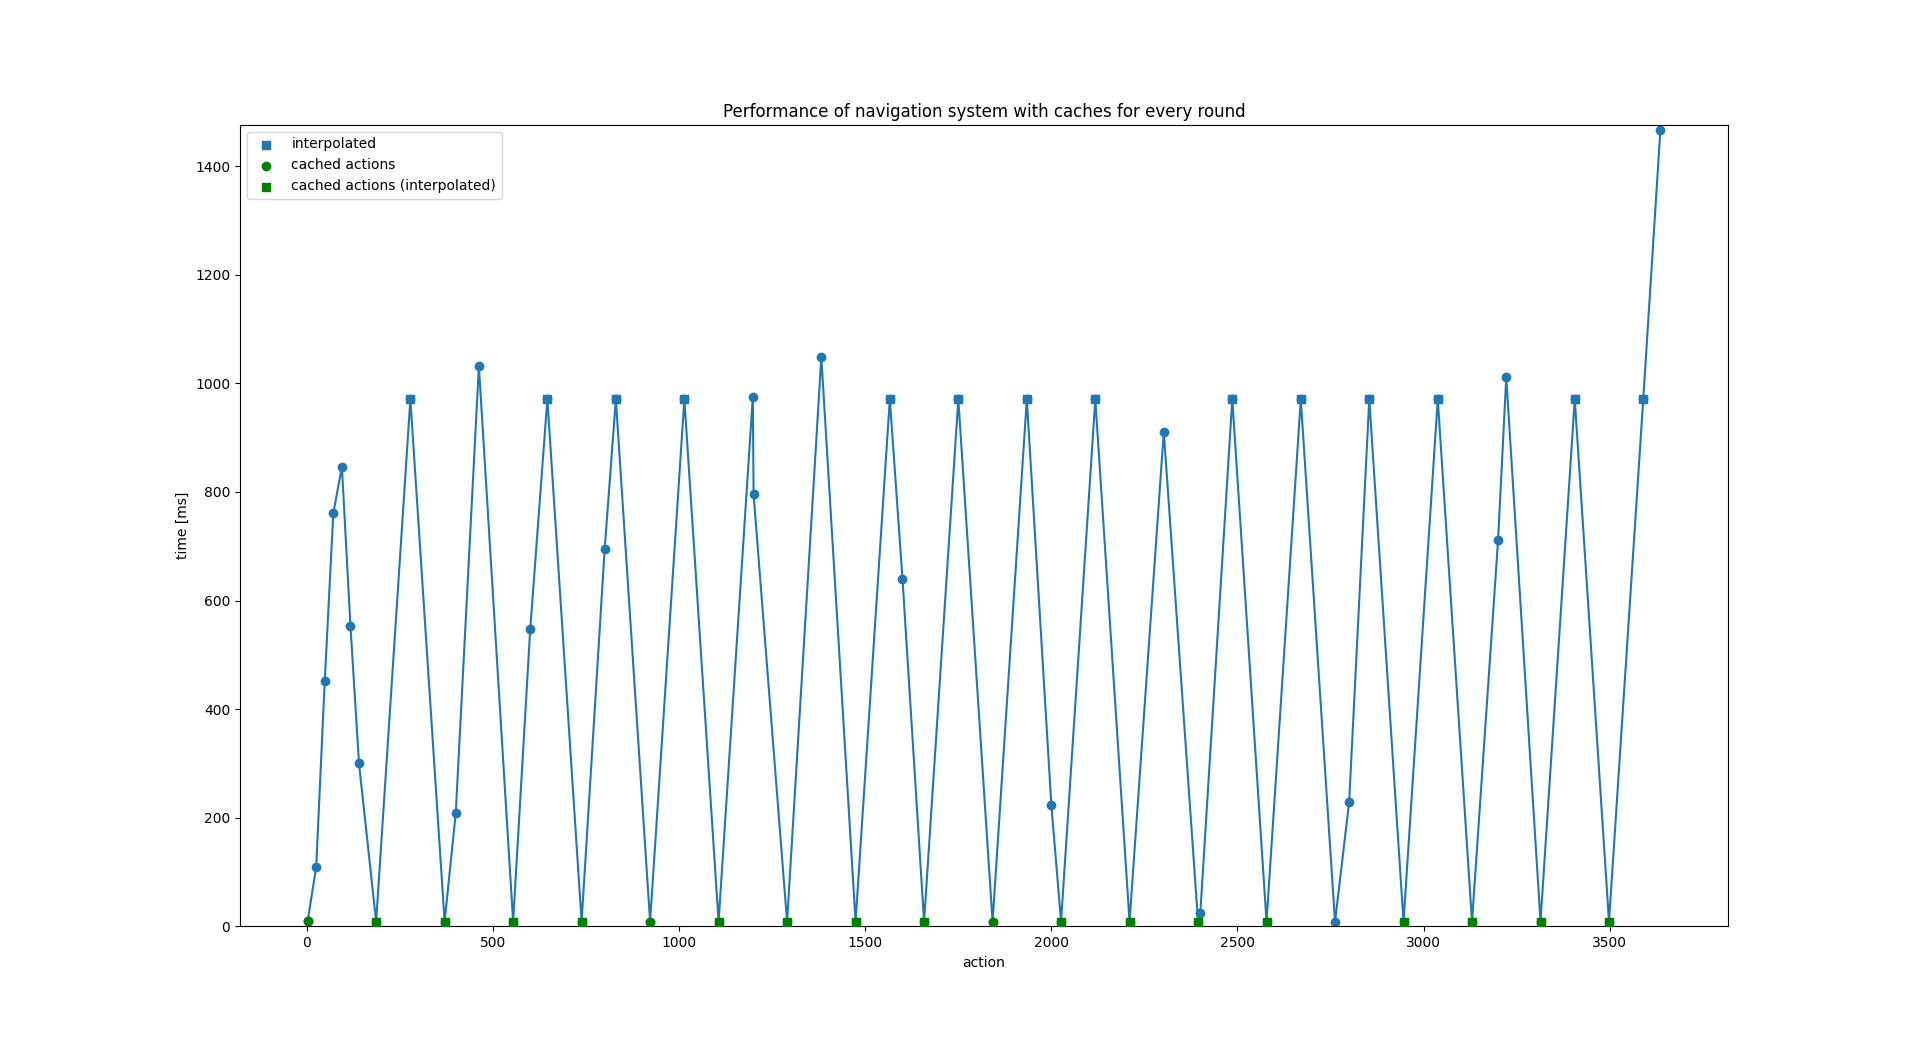
\includegraphics[width=\textwidth]{figures/pyplot/performance_navsystem-round-cache.png}
\caption{Performance of linear navigation system with caches for each round}
\label{fig:navsystem.performance.round}
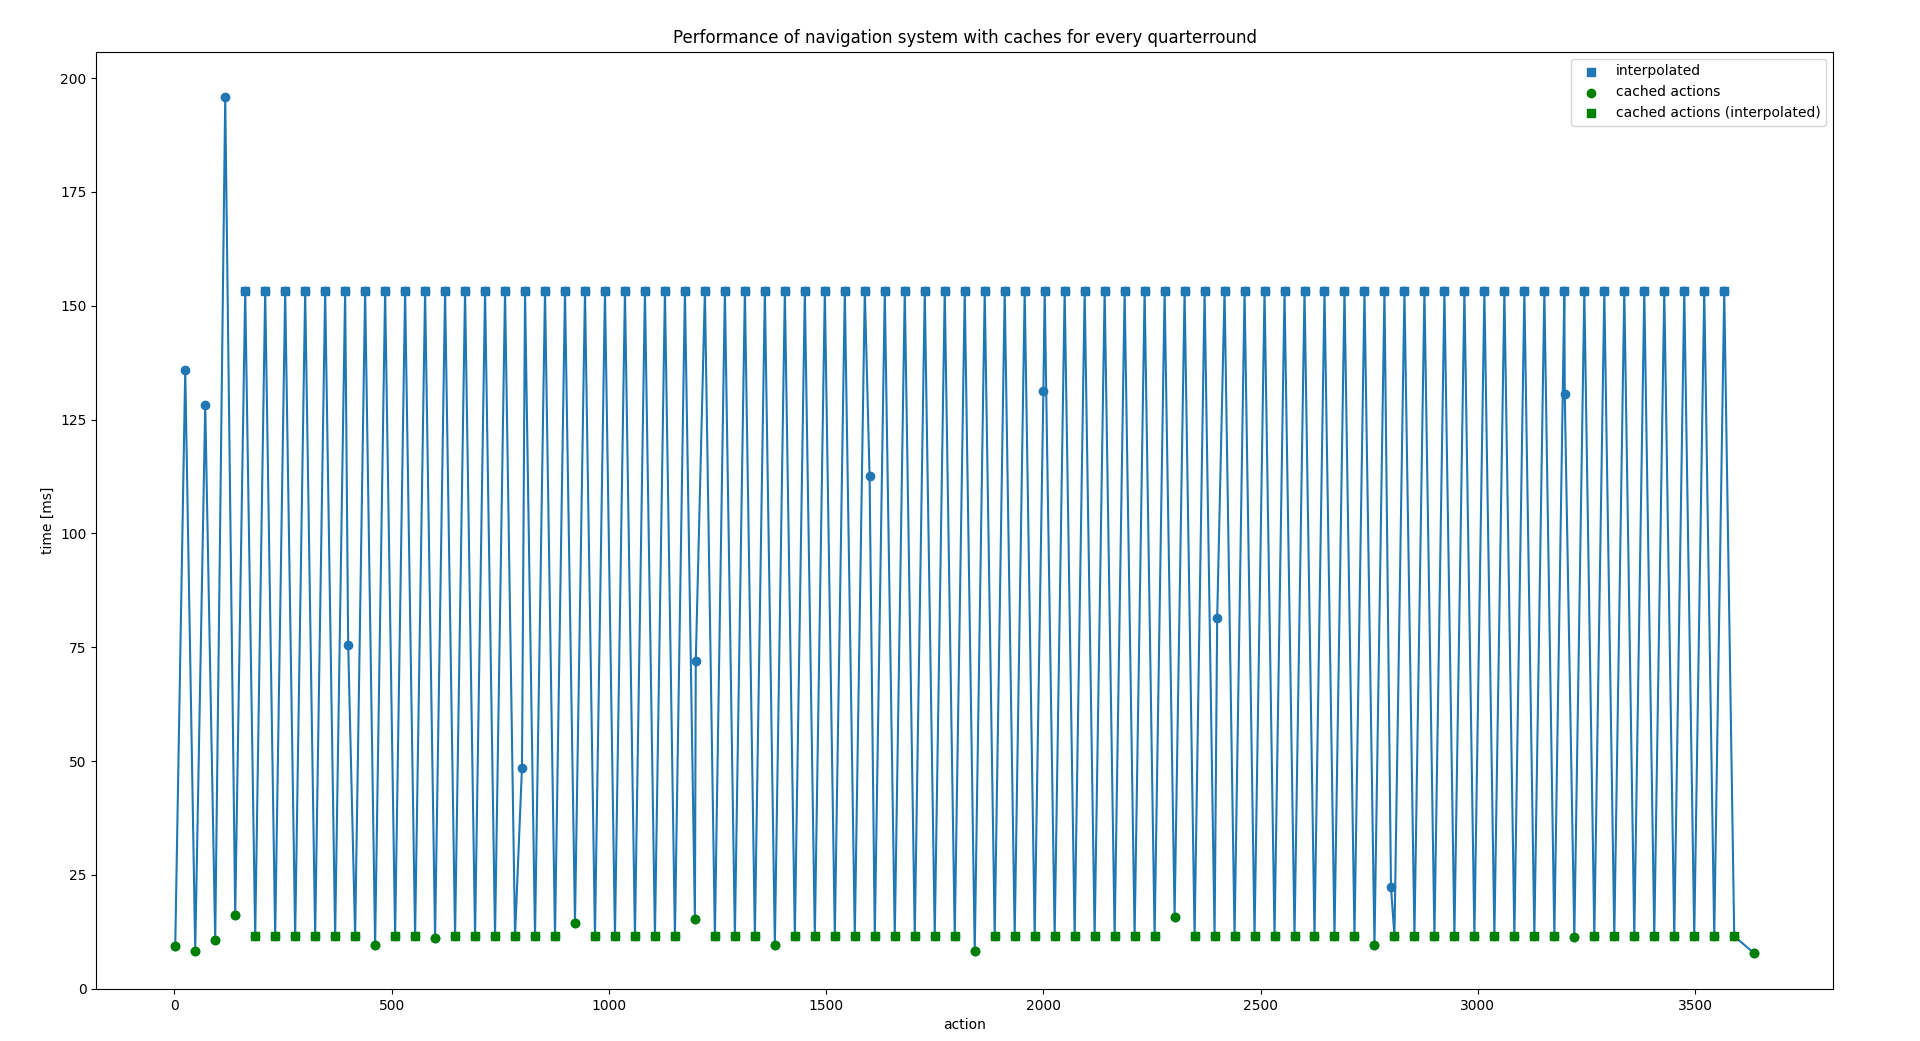
\includegraphics[width=\textwidth]{figures/pyplot/performance_navsystem-qr-cache.png}
\caption{Performance of linear navigation system with caches for each quarter-round}
\label{fig:navsystem.performance.qr}
\end{figure}

